\documentclass[11pt]{article}
\usepackage{arxiv}
\usepackage[utf8]{inputenc}
\usepackage{amsmath,amssymb,amsthm}
\usepackage{mathtools}
\usepackage{placeins}
\usepackage{graphicx}
\usepackage{float}
\usepackage{algorithm}
\usepackage{booktabs}
\usepackage{longtable}
\usepackage{array}
\usepackage{xcolor}
\usepackage[numbers,sort&compress]{natbib}
\usepackage[colorlinks=true,linkcolor=blue,citecolor=blue,urlcolor=blue]{hyperref}
\usepackage{cleveref}

\newtheorem{theorem}{Theorem}
\newtheorem{assumption}{Assumption}
\newcommand{\R}{\mathbb{R}}
\newcommand{\E}{\mathbb{E}}
\newcommand{\drift}{b}
\newcommand{\diff}{a}
\newcommand{\Lgen}{\mathcal{L}}
\newcommand{\xt}{X_t}
\newcommand{\Kj}{K_j}
\graphicspath{{figures/}}

\title{Symbolic Weak-Form Recovery of 2-D Stochastic Generators}

\author{%
  Sai Sathvik Gullipalli\thanks{Department of Computer Science Engineering, PES University
  (EC Campus), Bengaluru, KA 560100, India. \texttt{saisathvik127@gmail.com}} \quad
  Eshwar R A\thanks{Department of Computer Science Engineering, PES University
  (EC Campus), Bengaluru, KA 560100, India. \texttt{eshwarra5@gmail.com}} \quad
  Gajanan V. Honnavar\thanks{Department of Science and Humanities, PES University
  (EC Campus), Bengaluru, KA 560100, India. \texttt{gajanan.honnavar@pes.edu}.
  Corresponding author.}%
}
\date{}

\begin{document}
\maketitle

\begin{abstract}
Recovering the generators of two-dimensional It\^o diffusions from trajectory data remains
underexplored relative to the one-dimensional case, despite direct relevance to stochastic
volatility modeling, nonequilibrium statistical physics, and systems neuroscience. Building on
the weak-form spatial-kernel estimator of Eshwar and Honnavar~\cite{eshwar2026weak}, which is
unbiased and derivative-free in one dimension, we show that a naive component-wise extension to
two dimensions is ill-conditioned and recovers drift poorly.

We introduce a novel methodology for the discovery of such systems that retains the
spatial-Gaussian-kernel identity while adding six targeted mechanisms: standardized anisotropic
covariance-shaped kernels, a local-polynomial weak projection, adaptive-LASSO sparsification, a
Cholesky-parametrized diffusion fit that guarantees a positive-semidefinite tensor, a
generalized-least-squares drift pass that whitens by the first-pass diffusion tensor, and
multi-trajectory pooling with group-structured cross-validation. The key mathematical
contribution is proving that the GLS weights are $\mathcal{F}_{t_n}$-measurable, which preserves
the spatial-kernel unbiasedness theorem while improving efficiency without introducing
endogeneity.

We validate across 29 two-dimensional systems, achieving median drift error $\approx 0.23$,
off-diagonal diffusion cosine $\approx 0.99$, positive-semidefinite tensors at every grid point,
and zero false positives under our support criterion.
\end{abstract}

\noindent\textbf{Keywords:} stochastic generator recovery $\cdot$ weak-form sparse
identification $\cdot$ diffusion tensor $\cdot$ GLS whitening $\cdot$ leverage and circulation
$\cdot$ 2D It\^o diffusions

% ──────────────────────────────────────────────────────────────────────────────
\section{Introduction}\label{sec:intro}
% ──────────────────────────────────────────────────────────────────────────────

A central problem across quantitative finance, molecular dynamics, neuroscience, and climate
modelling is the \emph{inverse problem} for stochastic dynamics: given a discretely sampled,
noisy trajectory of a system, reconstruct the stochastic differential equation (SDE) that
generated it. The object that fully characterises a diffusion's local dynamics is its
infinitesimal generator $\Lgen f = \drift\!\cdot\!\nabla f + \tfrac{1}{2}\,\diff\!:\!\nabla^2 f$,
which encodes the drift vector $\drift$ and the diffusion tensor $\diff=\sigma\sigma^\top$.
Recovering $\Lgen$ symbolically---rather than as a black-box surrogate---exposes spectral gaps,
escape rates, leverage correlations, and probability currents directly.

The weak-form spatial-kernel estimator of Eshwar and Honnavar~\citep{eshwar2026weak} solves
this in one dimension. By projecting increments onto spatial Gaussian kernels $\Kj$ rather than
temporal test functions, it is unbiased (the kernel is $\mathcal{F}_{t_n}$-measurable, so the
It\^o noise integrates to zero in expectation), derivative-free, and produces an explicit
symbolic generator from a single shared design matrix. A companion
work~\citep{gullipalli2026heston} applied a restricted form to Heston stochastic volatility,
recovering the leverage correlation through a cross-variation target.

Extending this to genuinely two-dimensional, coupled, non-diagonal diffusions is the natural
next step the foundational paper lists as future work, and it is harder than it appears. A
faithful component-wise port of the 1D estimator to 2D---the ``naive port'' any reader would
try first---fails on the drift: the design matrix built from raw bivariate monomials over a
scale-disparate, localised state cloud is severely ill-conditioned, the unweighted normal
equations are statistically inefficient where the drift signal-to-noise ratio is low, and the
recovered diffusion tensor need not be positive semidefinite. We show these failures explicitly
(\Cref{sec:naive}) and then fix each with a targeted, conceptually motivated graft, yielding
\textbf{WG-SINDy}.

\paragraph{Contributions.}
(i) WG-SINDy, a weak-form 2D generator estimator built from six targeted grafts onto the 1D
spatial-kernel identity, recovering both drift components and all three independent entries of
the diffusion tensor symbolically (\Cref{sec:method}); (ii) a proof that the GLS drift-whitening
pass preserves the spatial-kernel unbiasedness of the 1D theory (\Cref{thm:unbiased});
(iii) a per-component \emph{necessity matrix} establishing that each of the six grafts solves a
distinct failure mode, framing the method as a structured extension of the weak form rather than
a collection of tricks (\Cref{sec:ablation}); and (iv) a broad validation over 29 2D systems
with per-system datasheets (\Cref{app:datasheets}), together with an explicit falsification
boundary.

\subsection{Scope of claims}\label{sec:scope}

We claim recovery over a broad class of \emph{identifiable} 2D It\^o diffusions: those whose
drift and diffusion lie in the chosen feature library, whose trajectories cover the state space,
and whose design matrix has full column rank. We do \emph{not} claim universal 2D recovery. We
name, and do not paper over, the limits where recovery fails: the risk-neutral log-price drift
$\mu-\tfrac{1}{2}v$ of stochastic-volatility models (signal-to-noise $\sim10^{-4}$ at financial
sampling rates), near-singular and rank-deficient diffusion tensors, Feller-violating boundaries,
non-spanning libraries, and under-covered state spaces. The diffusion tensor (not $\sigma$
itself) is the identifiable object, since $\sigma$ and $\sigma O$ for any orthogonal $O$ produce
the same $\diff=\sigma\sigma^\top$.

\subsection{Code and data availability}\label{sec:code}

A self-contained reproduction bundle (frozen estimator, all experiment runners, result tables,
figures, and this manuscript) is provided. Running \texttt{reproduce.sh} regenerates every
figure and table from fixed seeds.

% ──────────────────────────────────────────────────────────────────────────────
\section{Background}\label{sec:background}
% ──────────────────────────────────────────────────────────────────────────────

\subsection{It\^o diffusions and the generator}

Consider $\mathrm{d}\xt = \drift(\xt)\,\mathrm{d}t + \sigma(\xt)\,\mathrm{d}W_t$ on $\R^2$,
with diffusion tensor $\diff=\sigma\sigma^\top$ and generator
\begin{equation}
  \Lgen f = \drift_1\partial_1 f + \drift_2\partial_2 f
  + \tfrac{1}{2}\bigl(\diff_{11}\partial_{11}f
  + 2\diff_{12}\partial_{12}f + \diff_{22}\partial_{22}f\bigr).
\end{equation}
Recovery requires identifying five functions:
$\drift_1,\drift_2,\diff_{11},\diff_{12},\diff_{22}$. We write each as a sparse combination of
library features, $\drift_p=\Theta c^{(p)}$ and $\diff_{pq}=\Theta d^{(pq)}$.

\subsection{The 1D weak-form spatial-kernel estimator}

Given samples $\{X_{t_n}\}$ at step $\Delta t$, the 1D method~\citep{eshwar2026weak} places
spatial Gaussian kernels $\Kj$ over the state range and forms a single design
$A_{jk}=\sum_n \Kj(X_{t_n})f_k(X_{t_n})\Delta t$, shared by the drift system
$B^{(p)}_j=\sum_n \Kj\,\Delta X_n^{(p)}$ and the (cross-)variation system
$Q^{(pq)}_j=\sum_n \Kj\,\Delta X_n^{(p)}\Delta X_n^{(q)}$, with a finite-step bias correction
and lag-one observation-noise correction. Because $\Kj(X_{t_n})$ is
$\mathcal{F}_{t_n}$-measurable and the Brownian increment $\xi_n$ is independent of
$\mathcal{F}_{t_n}$, the tower property gives $\E[\Kj\sigma\xi_n]=0$, so the estimator is
unbiased---the property that temporal test functions famously lack.

\subsection{Related methods}

Stochastic SINDy and Kramers--Moyal estimators~\citep{boninsegna2018sparse} form each
regression row from a single-step increment, entangling signal and noise; Weak
SINDy~\citep{messenger2021weak} averages noise over test functions but was derived for
deterministic systems and does not treat the diffusion tensor; generator
EDMD~\citep{klus2020gedmd} estimates the operator densely and is neither sparse nor symbolic.
WG-SINDy retains the weak-form, sparse, symbolic, derivative-free identity while making the
full 2D tensor recoverable. We deliberately exclude mechanisms that would break this identity
(full gEDMD/eigenfunction targets, Milstein and It\^o--Taylor derivative targets, latent-state
Kalman/EM smoothing): the method is a weak-form extension, not a re-skinned operator method.

% ──────────────────────────────────────────────────────────────────────────────
\section{Methodology: WG-SINDy}\label{sec:method}
% ──────────────────────────────────────────────────────────────────────────────

WG-SINDy keeps the 1D identity and grafts six mechanisms; each is justified in
\Cref{sec:ablation} by its marginal contribution on the necessity matrix.

\paragraph{(G1) Standardized anisotropic kernels.}
States are standardised and kernel centres placed by $k$-means; the kernel bandwidth is the
empirical covariance scaled by $1.5$, so the kernel geometry matches the data cloud rather than
an isotropic ball. This fixes the severe ill-conditioning of the naive port on scale-disparate
systems.

\paragraph{(G2) Local-polynomial projection.}
The weak projection is local-polynomial of order two~\citep{fan1996local} rather than
local-constant (Nadaraya--Watson), which removes the $O(h^2)$ boundary bias that otherwise
corrupts tensor and drift estimates near the edge of the observed region.

\paragraph{(G3) Adaptive-LASSO sparsification.}
Feature selection uses adaptive LASSO with penalty weights inversely proportional to an initial
ridge estimate, promoting exact sparsity and reducing the false-positive rate relative to
unweighted $\ell_1$ regularisation.

\paragraph{(G4) Cholesky-parametrized diffusion fit.}
The diffusion is fit through a lower-triangular factor $L$ with $\diff=LL^\top$, so the
recovered tensor is positive semidefinite by construction~\citep{ledoit2004well}. Sparsity and
false-positive counts are defined on the factor entries; the reported symbolic tensor is the
expanded polynomial $LL^\top$.

\paragraph{(G5) GLS drift whitening.}
A first pass solves the drift and diffusion systems, then the drift is re-solved by
\emph{generalised least squares}: each weak row $j$ is weighted by the inverse of its
kernel-local noise variance
$V^{\mathrm{noise}}_j=\Delta t\int \Kj^2\,\hat\diff_{pp}\,\mathrm{d}\mu$. This is the core 2D
novelty: in one dimension there is no tensor to whiten by, but in two dimensions the
heteroscedastic, coupled noise across kernels makes the unweighted solve inefficient exactly
where the drift is weak. To keep the weights non-anticipative, the released code provides a
\emph{cross-fitting} option in which the weighting tensor for trajectory $r$ is estimated from
the remaining trajectories ($\hat\diff^{(-r)}$, leave-one-trajectory-out), making the weight
independent of the increment it multiplies (\Cref{thm:unbiased}(i)); the reported runs use
feasible in-sample weights, which \Cref{thm:unbiased}(ii) shows are asymptotically equivalent.

\paragraph{(G6) Multi-trajectory pooling.}
$R=16$ independent trajectories are stacked into a single design system and sparsified jointly
with group-structured cross-validation (one fold per trajectory). Pooling is the largest single
contributor to the in-scope score: the jump from $R=1$ to $R=16$ accounts for the majority of
the gap between the incremental ladder and full WG-SINDy (necessity-matrix row:
\texttt{NEC\_LOO\_MULTI\_TRAJECTORY}).

\begin{algorithm}[H]\small
\textbf{Algorithm 1: WG-SINDy} (six grafts on the 1D spatial-kernel identity).\\
\textit{Input:} $R$ trajectories $\{X^{(r)}_{t_n}\}$, step $\Delta t$, library $\Theta$,
kernel count $J$.\\[2pt]
(G1) Standardise states; place $J$ $k$-means centres; build anisotropic-covariance Gaussian
     kernels $\{\Kj\}$.\\
(G2) Form the shared local-polynomial (order-2) design matrix $A \in \R^{J \times p}$.\\
(G6) Stack all $R$ trajectories; form pooled drift target $B$ and cross-variation target $Q$
     with finite-step and lag-1 corrections.\\
\phantom{(G )} Solve pass-1 drift and diffusion systems.\\
(G4) Re-fit diffusion via Cholesky factor $L$ ($\diff = LL^\top$); guaranteed PSD.\\
(G5) Form GLS weights $1/V^{\mathrm{noise}}_j[\hat\diff]$ (cross-fitted option:
     $\hat\diff^{(-r)}$); re-solve drift (pass-2).\\
(G3) Adaptive-LASSO sparsification with group-structured cross-validation (one fold per
     trajectory).\\[2pt]
\textit{Output:} symbolic $\hat\Lgen$; read-outs: leverage
$\hat\diff_{12}/\sqrt{\hat\diff_{11}\hat\diff_{22}}$, fluctuation
$\hat\diff_{11},\hat\diff_{22}$, circulation from the antisymmetric drift Jacobian.
\end{algorithm}

\begin{theorem}[GLS preserves unbiasedness; feasible GLS is asymptotically
equivalent]\label{thm:unbiased}
\emph{(i) Cross-fitted GLS.} If the weighting tensor for trajectory $r$ is estimated from the
other trajectories, $\hat\diff^{(-r)}$, then the weight
$w_j^{(-r)}=1/V^{\mathrm{noise}}_j[\hat\diff^{(-r)}]$ is independent of trajectory $r$'s own
increments, so
$\E[\,w_j^{(-r)}\Kj(X_{t_n})\sigma(X_{t_n})\xi_n\mid\mathcal{F}_{t_n}\,]=0$ and the
cross-fitted GLS drift estimator is exactly unbiased and consistent under the standing
ergodicity, coverage, and full-rank conditions.

\emph{(ii) Feasible (in-sample) GLS.} With weights built from the pooled first-pass $\hat\diff$,
the weight is not strictly $\mathcal{F}_{t_n}$-measurable; however, since $\hat\diff\to\diff$,
the induced endogeneity bias is $o_p(1)$ at the rate of the tensor-estimation error, so feasible
GLS is asymptotically equivalent to oracle GLS. In both cases GLS \emph{reduces variance}
relative to the unweighted weak regression and attains feasible-GLS efficiency under oracle
support and regularity; we do not claim exact finite-sample efficiency.
\end{theorem}

\begin{proof}[Proof sketch]
(i) $w_j^{(-r)}\Kj(X_{t_n})\sigma(X_{t_n})$ is, conditional on $\mathcal{F}_{t_n}$ and the
held-out fold, deterministic in trajectory $r$, while $\xi_n\perp\mathcal{F}_{t_n}$; the tower
property gives conditional mean zero, hence unconditional mean zero. Consistency follows from
the ergodic limit of the weighted normal equations as in the unweighted case.

(ii) Writing $w_j=w_j^\star+(w_j-w_j^\star)$ with the oracle weight $w_j^\star$, the first term
is unbiased by part (i) and the second contributes a bias of order
$\|\hat\diff-\diff\|=o_p(1)$. The released code supports cross-fitted
(leave-one-trajectory-out) weights, to which part (i) applies; the reported feasible-GLS runs
are covered by part (ii).
\end{proof}

\subsection{Explicit corrections and the Cholesky diffusion fit}\label{sec:cholesky}

\paragraph{Finite-step and lag-one corrections.}
The raw cross-variation $\sum_n \Kj\,\Delta X_n^{(p)}\Delta X_n^{(q)}$ estimates
$\int \Kj\diff_{pq}\,\mathrm{d}t$ to leading order but carries an $O(\Delta t^2)$ drift-squared
bias. Squaring the Euler--Maruyama increment gives
$\Delta X_n\Delta X_n^\top=\diff\,\Delta t+\drift\drift^\top\Delta t^2
+(\text{mean-zero }O(\Delta t^{3/2}))$, so after the drift pass we subtract the corrected term
$Q^{(pq),\mathrm{corr}}_j=\sum_n
\Kj\bigl[\Delta X_n^{(p)}\Delta X_n^{(q)}-\hat\drift_p(X_n)\hat\drift_q(X_n)\Delta t^2\bigr]$.
Under additive observation noise $\tilde X=X+\eta$, the lag-zero quadratic variation is inflated
by $2\Sigma_\eta$ while the lag-one product
$\E[\Delta\tilde X_n\Delta\tilde X_{n+1}^\top]=-\Sigma_\eta$ is not; we estimate
$\hat\Sigma_\eta=-\tfrac{1}{N-1}\sum_n\Delta\tilde X_n\Delta\tilde X_{n+1}^\top$ and subtract
$2\hat\Sigma_\eta$ from the per-row outer products before projection. Both corrections act
entrywise on the $2\times2$ tensor, including the off-diagonal.

\paragraph{Cholesky fit.}
To guarantee a positive-semidefinite recovered tensor we parametrise $\diff=LL^\top$ with
lower-triangular
$L=\begin{psmallmatrix}\ell_{11}&0\\ \ell_{21}&\ell_{22}\end{psmallmatrix}$ and fit the
\emph{factor entries} $\ell_{11},\ell_{21},\ell_{22}$ as sparse library expansions
$\ell_{ab}=\Theta\beta^{(ab)}$. Because
$\diff_{11}=\ell_{11}^2,\ \diff_{12}=\ell_{11}\ell_{21},\ \diff_{22}=\ell_{21}^2+\ell_{22}^2$
are quadratic in the factors, the corrected cross-variation targets are matched by a separable
nonlinear least-squares problem,
$\min_{\beta}\sum_j\bigl\|Q^{\mathrm{corr}}_j-(LL^\top)(\,\cdot\,;\beta)\bigr\|^2$, solved by
alternating ridge-regularised updates initialised from the unconstrained linear $\diff$-fit.
\emph{Sparsity and the false-positive count are defined on the factor entries $\beta^{(ab)}$};
the \emph{reported symbolic tensor} is the expanded polynomial $LL^\top$. The Cholesky map
introduces no first-order bias in $\diff_{12}$ when the true tensor is in range (quantified on
the non-diagonal-Cholesky datasheet); near rank deficiency it trades a small magnitude bias for
guaranteed positive semidefiniteness.

\subsection{Metrics and the support rule}\label{sec:metrics}

For a recovered function $\hat g$ against truth $g$ on a grid weighted by the empirical
stationary measure $\mu$, the relative error is
$\|\hat g-g\|_{L^2(\mu)}/\|g\|_{L^2(\mu)}$; we report the \emph{drift} error as the mean over
$\drift_1,\drift_2$ and the \emph{tensor} error as the mean over
$\diff_{11},\diff_{12},\diff_{22}$ (Frobenius). The \emph{off-diagonal cosine} is
$\langle\hat\diff_{12},\diff_{12}\rangle_\mu/(\|\hat\diff_{12}\|\,\|\diff_{12}\|)$; the
\emph{PSD-valid fraction} is the share of grid points with $\hat\diff\succeq0$; the
\emph{generator-action error} compares $\hat\Lgen f$ to $\Lgen f$ on the test set
$f\in\{x,y,x^2,xy,y^2\}$. We additionally report a \emph{support F1} (precision/recall of the
selected term set) so that a system with low field error but an incorrect symbolic support is
scored honestly---the axis on which a named limit fails is stated in its datasheet. The aggregate
``in-scope score'' used in some figures is a secondary convenience defined as
$1-\mathrm{clip}_{[0,1]}(\text{drift }L^2)$ averaged with
$1-\mathrm{clip}_{[0,1]}(\text{tensor }L^2)$ and the PSD fraction; all conclusions are also
reported on the primary metrics above with bootstrap confidence intervals.

\paragraph{Reporting recovered coefficients across seeds.}
Each coefficient is estimated over $10$ seeds. We report, per term, its \emph{selection rate}
(fraction of seeds in which it is selected) and the \emph{median value over the seeds in which
it is selected} (with a bootstrap CI), \emph{not} the plain median over all seeds. The plain
cross-seed median conflates a coefficient's value with its selection frequency: a
weakly-identified but genuine term selected in a minority of seeds is reported as exactly zero,
misrepresenting an intermittently-recovered term as a missed one. Under this reporting the
dominant terms recover to a few percent (e.g.\ correlated-OU drift and off-diagonal at selection
rate $1.0$), and weakly-identified secondary terms are shown with their true selection rate
rather than hidden in a zero median---e.g.\ the Duffing damping $-0.35\,y$ recovers at
$\approx-0.33$ (selection rate $0.7$) and the Maier--Stein $-x^2y$ at $\approx-1.0$ (rate
$0.7$), while genuinely weak terms such as the Maier--Stein $-0.35\,xy^2$ (rate $0$--$0.3$)
are reported as such.

\paragraph{Support and false-positive rule.}
Columns of the design are $\ell_2$-normalised; a term is \emph{selected} if its post-debias
coefficient exceeds $\tau=10^{-3}$ of the largest selected coefficient for that target. A
\emph{false positive} is a selected term whose true coefficient is zero; near-zero true
coefficients (those below the same $\tau$ relative scale) are treated as inactive. For the
diffusion, selection is counted on the Cholesky factor entries. False positives are counted
\emph{after} debiasing and STLSQ pruning. This rule is fixed across the whole zoo and is not
tuned per system.

\paragraph{Three read-outs.}
The recovered generator is read three ways: the off-diagonal $\hat\diff_{12}$ gives the
\emph{leverage} correlation (financial systems); the diagonal $\hat\diff_{11},\hat\diff_{22}$
give the \emph{fluctuation} field and position-dependent relaxation; and the antisymmetric part
of the drift Jacobian gives a \emph{local rotational-drift diagnostic} of non-reversibility.
(This equals the stationary probability current
$J=\drift\pi-\tfrac{1}{2}\nabla\!\cdot(\diff\pi)$ only for additive-noise/linear systems; for
state-dependent diffusion it is a diagnostic, not the full current.)

% ──────────────────────────────────────────────────────────────────────────────
\section{Results}\label{sec:results}
% ──────────────────────────────────────────────────────────────────────────────

\subsection{Ground-truth recovery across the zoo}\label{sec:showcase}

\Cref{tab:master} is the navigation layer: every 2D system, its in-scope/limit status, and the
recovered-vs-true metrics over $10$ seeds. Of the 29 systems, nineteen pass the metric gate, two
are scoped reviews (low-SNR drift with strong tensor/leverage), and eight are named limits. No
system exhibits a false positive under the support rule defined above. Representative
recovered-vs-true field comparisons appear in the per-system datasheets (\Cref{app:datasheets});
each recovers the symbolic coefficients to a few percent.

\begin{table}[t]\centering\small
\caption{Master system index (navigation layer). Recovery metrics are medians over $n=10$ seeds at the frozen
WG-SINDy configuration. ``Drift'' is the $L^2(\mu)$ relative drift error; ``Tensor'' the relative diffusion-tensor
error; ``$a_{12}$cos'' the off-diagonal cosine (``--'' where diffusion is diagonal, so $a_{12}\equiv0$);
``PSD'' the fraction of grid points with a positive-semidefinite recovered tensor; ``FP'' the false-positive
count. $\checkmark$ PASS, $\circ$ scoped review, $\times$ named physical limit. Each system links to its
datasheet in \Cref{app:datasheets}.}\label{tab:master}
\begin{tabular}{l l c c c c c c}
\toprule
System & Family/Tier & Drift & Tensor & $a_{12}$cos & PSD & FP & Verdict \\
\midrule
\multicolumn{8}{l}{\textit{Linear Ornstein--Uhlenbeck}}\\
\hyperref[sec:v62-indep-ou]{Independent OU} & linear/1 & 0.098 & 0.033 & -- & 1.00 & 0 & $\checkmark$ \\
\hyperref[sec:v62-correlated-ou]{Correlated OU} & linear/1 & 0.136 & 0.051 & 1.000 & 1.00 & 0 & $\checkmark$ \\
\hyperref[sec:v62-coupled-ou]{Coupled OU} & linear/1 & 0.214 & 0.028 & -- & 1.00 & 0 & $\checkmark$ \\
\hyperref[sec:v62-two-factor-vasicek]{Two-factor Vasicek} & linear/9 & 0.350 & --$^\dagger$ & -- & 1.00 & 0 & $\circ$ \\
\midrule
\multicolumn{8}{l}{\textit{Rotational / non-reversible}}\\
\hyperref[sec:v62-rotational-ou]{Rotational OU} & rotational/2 & 0.058 & 0.038 & -- & 1.00 & 0 & $\checkmark$ \\
\hyperref[sec:v62-spiral-sink-corr]{Spiral sink + corr.\ noise} & rotational/2 & 0.078 & 0.043 & 1.000 & 1.00 & 0 & $\checkmark$ \\
\hyperref[sec:v62-nongradient-circulation]{Non-gradient circulation} & rotational/3 & 0.239 & 0.024 & -- & 1.00 & 0 & $\checkmark$ \\
\midrule
\multicolumn{8}{l}{\textit{Bistable / gradient}}\\
\hyperref[sec:v62-double-well-transverse]{Double well + transverse} & bistable/3 & 0.226 & 0.024 & -- & 1.00 & 0 & $\checkmark$ \\
\hyperref[sec:v62-gradient-potential]{Gradient potential} & bistable/3 & 0.246 & 0.024 & -- & 1.00 & 0 & $\checkmark$ \\
\hyperref[sec:v62-maier-stein]{Maier--Stein} & bistable/8 & 0.235 & 0.038 & -- & 1.00 & 0 & $\checkmark$ \\
\hyperref[sec:v62-duffing]{Duffing oscillator} & bistable/8 & 0.240 & 0.031 & -- & 1.00 & 0 & $\checkmark$ \\
\hyperref[sec:v62-mueller-brown]{M\"uller--Brown} & bistable/8 & 1.826 & 0.075 & -- & 1.00 & 0 & $\times$ \\
\midrule
\multicolumn{8}{l}{\textit{Multiplicative / state-dependent diffusion}}\\
\hyperref[sec:v62-diag-multiplicative]{Diagonal multiplicative} & multipl./4 & 0.200 & 0.112 & -- & 1.00 & 0 & $\checkmark$ \\
\hyperref[sec:v62-nondiag-cholesky]{Non-diagonal Cholesky} & multipl./4 & 0.204 & 0.079 & 0.988 & 1.00 & 0 & $\checkmark$ \\
\hyperref[sec:v62-near-singular]{Near-singular tensor} & multipl./4 & 0.870 & 1.505 & 0.724 & 1.00 & 0 & $\times$ \\
\midrule
\multicolumn{8}{l}{\textit{Financial / stochastic volatility}}\\
\hyperref[sec:v62-heston-logsv]{Log-Heston} & financial/5 & 0.143 & 0.054 & 0.999 & 1.00 & 0 & $\checkmark$ \\
\hyperref[sec:v62-heston-sv]{Heston $(S,V)$} & financial/5 & 0.273 & 0.089 & 0.993 & 1.00 & 0 & $\checkmark$ \\
\hyperref[sec:v62-cir-pair]{CIR pair} & financial/5 & 0.393 & 0.116 & 0.995 & 1.00 & 0 & $\checkmark$ \\
\hyperref[sec:v62-sabr]{SABR} & financial/9 & --$^\ddagger$ & 0.195 & 0.990 & 1.00 & 0 & $\times$ \\
\hyperref[sec:v62-gbm-2d]{Correlated 2D GBM} & financial/9 & 2.49 & 0.096 & 0.997 & 1.00 & 0 & $\circ$ \\
\midrule
\multicolumn{8}{l}{\textit{Stochastic limit cycles}}\\
\hyperref[sec:v62-van-der-pol]{Van der Pol} & limit-cycle/7 & 0.066 & 0.040 & -- & 1.00 & 0 & $\checkmark$ \\
\hyperref[sec:v62-fitzhugh-nagumo]{FitzHugh--Nagumo} & limit-cycle/7 & 0.205 & 0.040 & -- & 1.00 & 0 & $\checkmark$ \\
\hyperref[sec:v62-stuart-landau]{Stuart--Landau} & limit-cycle/7 & 0.126 & 0.018 & -- & 1.00 & 0 & $\checkmark$ \\
\hyperref[sec:v62-brusselator]{Brusselator} & limit-cycle/7 & 0.013 & 0.067 & -- & 1.00 & 0 & $\checkmark$ \\
\midrule
\multicolumn{8}{l}{\textit{Honest limits (named, reported)}}\\
\hyperref[sec:v62-underdamped-langevin]{Underdamped Langevin} & limit/6 & 0.157 & 0.563 & -- & 1.00 & 0 & $\times$ \\
\hyperref[sec:v62-near-boundary-heston]{Near-boundary Heston} & limit/6 & 1.413 & 0.267 & 0.982 & 1.00 & 0 & $\times$ \\
\hyperref[sec:v62-nonpoly-drift]{Non-polynomial drift} & limit/6 & 0.210 & 0.037 & -- & 1.00 & 0 & $\times$ \\
\hyperref[sec:v62-bad-coverage]{Bad coverage} & limit/6 & 0.815 & 0.784 & -- & 1.00 & 0 & $\times$ \\
\hyperref[sec:v62-too-large-dt]{Too-large $\Delta t$} & limit/6 & 0.098 & 0.119 & -- & 1.00 & 0 & $\times$ \\
\bottomrule
\end{tabular}
\\[2pt]
\footnotesize $^\dagger$ Constant tiny tensor: relative-$L^2$ is degenerate; absolute error is small (see datasheet).
$^\ddagger$ SABR is driftless ($b\equiv0$); the drift relative error is undefined while tensor and leverage are recovered.
\end{table}


\paragraph{Symbolic coefficient recovery, true vs.\ recovered vs.\ baseline.}
\Cref{tab:coeff-recovery} answers the question directly: for each system it lists the
coefficients of the equation \emph{used to generate} the data, the coefficients \emph{returned}
by the WG-SINDy pipeline (median over the seeds in which each term is selected, with its
selection rate), and a matched Kramers--Moyal / Stochastic-SINDy baseline on the same library.
Across the linear, coupled, rotational, limit-cycle, and multiplicative families every dominant
term is recovered to a few percent at selection rate $1.0$, and WG-SINDy matches or beats the
baseline on the nonlinear and off-diagonal terms (e.g.\ the Stuart--Landau cubic terms and the
Maier--Stein $-x^2y$, where the baseline degrades or flips sign); the only intermittently
selected terms are genuinely low-SNR (e.g.\ Maier--Stein $-0.35\,xy^2$), which the baseline
also misses.

% Auto-generated from results/v10/coeff_recovery_R32.csv
\begin{longtable}{l l r r r r}
\caption{Symbolic coefficient recovery under the pooled R=32 rerun. Each row reports the coefficient used to generate the data, WG-SINDy as the median over selected seeds, the selection rate over four independent pooled fits, and a matched Kramers--Moyal / stochastic-SINDy baseline on the same library.}\label{tab:coeff-recovery}\\
\toprule
System & Term & True & WG-SINDy & sel & KM-base \\ \midrule \endfirsthead
\toprule System & Term & True & WG-SINDy & sel & KM-base \\ \midrule \endhead
\bottomrule \endfoot
\multicolumn{6}{l}{\textit{Correlated OU}}\\
  & b1:\,$x$ & $-1.000$ & $-0.979$ & 1.00 & $-1.008$ \\
  & b2:\,$y$ & $-1.500$ & $-1.486$ & 1.00 & $-1.509$ \\
  & a11:\,$\mathbf{1}$ & $+1.000$ & $+0.991$ & 1.00 & $+0.983$ \\
  & a12:\,$\mathbf{1}$ & $-0.480$ & $-0.475$ & 1.00 & $-0.472$ \\
  & a22:\,$\mathbf{1}$ & $+0.640$ & $+0.631$ & 1.00 & $+0.628$ \\
\addlinespace
\multicolumn{6}{l}{\textit{Coupled OU}}\\
  & b1:\,$x$ & $-1.000$ & $-0.999$ & 1.00 & $-1.001$ \\
  & b1:\,$y$ & $+0.500$ & $+0.514$ & 1.00 & $+0.486$ \\
  & b2:\,$x$ & $+0.500$ & $+0.503$ & 1.00 & $+0.483$ \\
  & b2:\,$y$ & $-1.000$ & $-0.988$ & 1.00 & $-0.995$ \\
  & a11:\,$\mathbf{1}$ & $+1.000$ & $+0.990$ & 1.00 & $+0.986$ \\
  & a22:\,$\mathbf{1}$ & $+1.000$ & $+0.989$ & 1.00 & $+0.983$ \\
\addlinespace
\multicolumn{6}{l}{\textit{Rotational OU}}\\
  & b1:\,$x$ & $-1.000$ & $-1.013$ & 1.00 & $-1.008$ \\
  & b1:\,$y$ & $-2.000$ & $-1.999$ & 1.00 & $-2.010$ \\
  & b2:\,$x$ & $+2.000$ & $+2.004$ & 1.00 & $+1.972$ \\
  & b2:\,$y$ & $-1.000$ & $-0.993$ & 1.00 & $-0.992$ \\
  & a11:\,$\mathbf{1}$ & $+1.000$ & $+0.989$ & 1.00 & $+0.987$ \\
  & a22:\,$\mathbf{1}$ & $+1.000$ & $+0.988$ & 1.00 & $+0.983$ \\
\addlinespace
\multicolumn{6}{l}{\textit{Spiral sink + correlated noise}}\\
  & b1:\,$x$ & $-1.000$ & $-0.990$ & 1.00 & $-1.016$ \\
  & b1:\,$y$ & $-1.500$ & $-1.492$ & 1.00 & $-1.478$ \\
  & b2:\,$x$ & $+1.500$ & $+1.495$ & 1.00 & $+1.511$ \\
  & b2:\,$y$ & $-1.000$ & $-1.018$ & 1.00 & $-1.017$ \\
  & a11:\,$\mathbf{1}$ & $+1.000$ & $+0.997$ & 1.00 & $+0.991$ \\
  & a12:\,$\mathbf{1}$ & $-0.400$ & $-0.394$ & 1.00 & $-0.392$ \\
  & a22:\,$\mathbf{1}$ & $+0.640$ & $+0.627$ & 1.00 & $+0.626$ \\
\addlinespace
\multicolumn{6}{l}{\textit{Van der Pol}}\\
  & b1:\,$y$ & $+1.000$ & $+0.997$ & 1.00 & $+0.995$ \\
  & b2:\,$x$ & $-1.000$ & $-0.996$ & 1.00 & $-1.003$ \\
  & b2:\,$y$ & $+1.200$ & $+1.194$ & 1.00 & $+1.209$ \\
  & b2:\,$x^2y$ & $-1.200$ & $-1.196$ & 1.00 & $-1.200$ \\
  & a11:\,$\mathbf{1}$ & $+0.122$ & $+0.122$ & 1.00 & $+0.124$ \\
  & a22:\,$\mathbf{1}$ & $+0.122$ & $+0.122$ & 1.00 & $+0.188$ \\
\addlinespace
\multicolumn{6}{l}{\textit{Stuart-Landau}}\\
  & b1:\,$x$ & $+1.000$ & $+0.988$ & 1.00 & $+0.975$ \\
  & b1:\,$y$ & $-1.500$ & $-1.507$ & 1.00 & $-1.551$ \\
  & b1:\,$x^3$ & $-1.000$ & $-0.978$ & 1.00 & $-0.960$ \\
  & b1:\,$xy^2$ & $-1.000$ & $-0.993$ & 1.00 & $-0.970$ \\
  & b2:\,$x$ & $+1.500$ & $+1.494$ & 1.00 & $+1.439$ \\
  & b2:\,$y$ & $+1.000$ & $+0.997$ & 1.00 & $+1.063$ \\
  & b2:\,$x^2y$ & $-1.000$ & $-1.005$ & 1.00 & $-1.040$ \\
  & b2:\,$y^3$ & $-1.000$ & $-0.984$ & 1.00 & $-1.056$ \\
  & a11:\,$\mathbf{1}$ & $+0.078$ & $+0.078$ & 1.00 & $+0.077$ \\
  & a22:\,$\mathbf{1}$ & $+0.078$ & $+0.079$ & 1.00 & $+0.077$ \\
\addlinespace
\multicolumn{6}{l}{\textit{Brusselator}}\\
  & b1:\,$\mathbf{1}$ & $+1.000$ & $+0.868$ & 1.00 & $+0.789$ \\
  & b1:\,$x$ & $-3.600$ & $-3.444$ & 1.00 & $-3.391$ \\
  & b1:\,$x^2y$ & $+1.000$ & $+1.045$ & 1.00 & $+1.017$ \\
  & b2:\,$x$ & $+2.600$ & $+2.467$ & 1.00 & $+2.025$ \\
  & b2:\,$x^2y$ & $-1.000$ & $-1.039$ & 1.00 & $-1.040$ \\
  & a11:\,$\mathbf{1}$ & $+0.014$ & $+0.015$ & 1.00 & $-0.472$ \\
  & a22:\,$\mathbf{1}$ & $+0.014$ & $+0.016$ & 1.00 & $-0.529$ \\
\addlinespace
\multicolumn{6}{l}{\textit{Duffing oscillator}}\\
  & b1:\,$y$ & $+1.000$ & $+1.002$ & 1.00 & $+1.008$ \\
  & b2:\,$x$ & $+1.000$ & $+0.964$ & 1.00 & $+0.973$ \\
  & b2:\,$y$ & $-0.350$ & $-0.354$ & 1.00 & $-0.379$ \\
  & b2:\,$x^3$ & $-1.000$ & $-0.976$ & 1.00 & $-0.983$ \\
  & a11:\,$\mathbf{1}$ & $+0.090$ & $+0.090$ & 1.00 & $+0.090$ \\
  & a22:\,$\mathbf{1}$ & $+0.090$ & $+0.090$ & 1.00 & $+0.082$ \\
\addlinespace
\multicolumn{6}{l}{\textit{Maier-Stein}}\\
  & b1:\,$x$ & $+1.000$ & $+0.975$ & 1.00 & $+0.987$ \\
  & b1:\,$x^3$ & $-1.000$ & $-0.977$ & 1.00 & $-0.974$ \\
  & b1:\,$xy^2$ & $-0.350$ & $+0.000$ & 0.00 & $-1.053$ \\
  & b2:\,$y$ & $-1.000$ & $-0.874$ & 1.00 & $-1.218$ \\
  & b2:\,$x^2y$ & $-1.000$ & $-1.095$ & 1.00 & $-0.911$ \\
  & a11:\,$\mathbf{1}$ & $+0.122$ & $+0.122$ & 1.00 & $+0.125$ \\
  & a22:\,$\mathbf{1}$ & $+0.122$ & $+0.123$ & 1.00 & $+0.122$ \\
\addlinespace
\multicolumn{6}{l}{\textit{Gradient potential}}\\
  & b1:\,$x$ & $+1.000$ & $+0.900$ & 1.00 & $+1.012$ \\
  & b1:\,$x^3$ & $-1.000$ & $-0.974$ & 1.00 & $-1.009$ \\
  & b1:\,$xy^2$ & $-0.500$ & $+0.000$ & 0.00 & $-0.560$ \\
  & b2:\,$y$ & $-1.000$ & $-1.037$ & 1.00 & $-1.028$ \\
  & b2:\,$x^2y$ & $-0.500$ & $-0.469$ & 1.00 & $-0.541$ \\
  & a11:\,$\mathbf{1}$ & $+0.245$ & $+0.489$ & 1.00 & $+0.486$ \\
  & a22:\,$\mathbf{1}$ & $+0.245$ & $+0.491$ & 1.00 & $+0.483$ \\
\addlinespace
\multicolumn{6}{l}{\textit{Diagonal multiplicative}}\\
  & b1:\,$x$ & $-1.000$ & $-0.980$ & 1.00 & $-1.029$ \\
  & b2:\,$y$ & $-1.000$ & $-1.005$ & 1.00 & $-0.998$ \\
  & a11:\,$\mathbf{1}$ & $+0.500$ & $+0.499$ & 1.00 & $+0.497$ \\
  & a11:\,$x^2$ & $+0.100$ & $+0.100$ & 1.00 & $+0.113$ \\
  & a22:\,$\mathbf{1}$ & $+0.400$ & $+0.399$ & 1.00 & $+0.398$ \\
  & a22:\,$y^2$ & $+0.100$ & $+0.097$ & 1.00 & $+0.111$ \\
\addlinespace
\multicolumn{6}{l}{\textit{Non-diagonal Cholesky}}\\
  & b1:\,$x$ & $-1.000$ & $-0.982$ & 1.00 & $-0.985$ \\
  & b2:\,$y$ & $-1.000$ & $-1.011$ & 1.00 & $-1.017$ \\
  & a12:\,$xy$ & $+0.100$ & $+0.111$ & 1.00 & $+0.116$ \\
  & a11:\,$\mathbf{1}$ & $+0.250$ & $+0.250$ & 1.00 & $+0.250$ \\
  & a22:\,$\mathbf{1}$ & $+0.160$ & $+0.160$ & 1.00 & $+0.159$ \\
\addlinespace
\end{longtable}


\FloatBarrier
\subsection{The 1D method fails in 2D}\label{sec:naive}

The naive component-wise port (B0, the published 1D code applied to each of the five 2D
functions, no grafts) fails on drift for scale-disparate and correlated systems: the design
condition number explodes, low-SNR drift components are overwhelmed by spurious high-degree
terms, and the tensor is not guaranteed positive semidefinite. \Cref{fig:naive} maps the failure
across the zoo. This motivates each graft.

\begin{figure}[t]
  \centering
  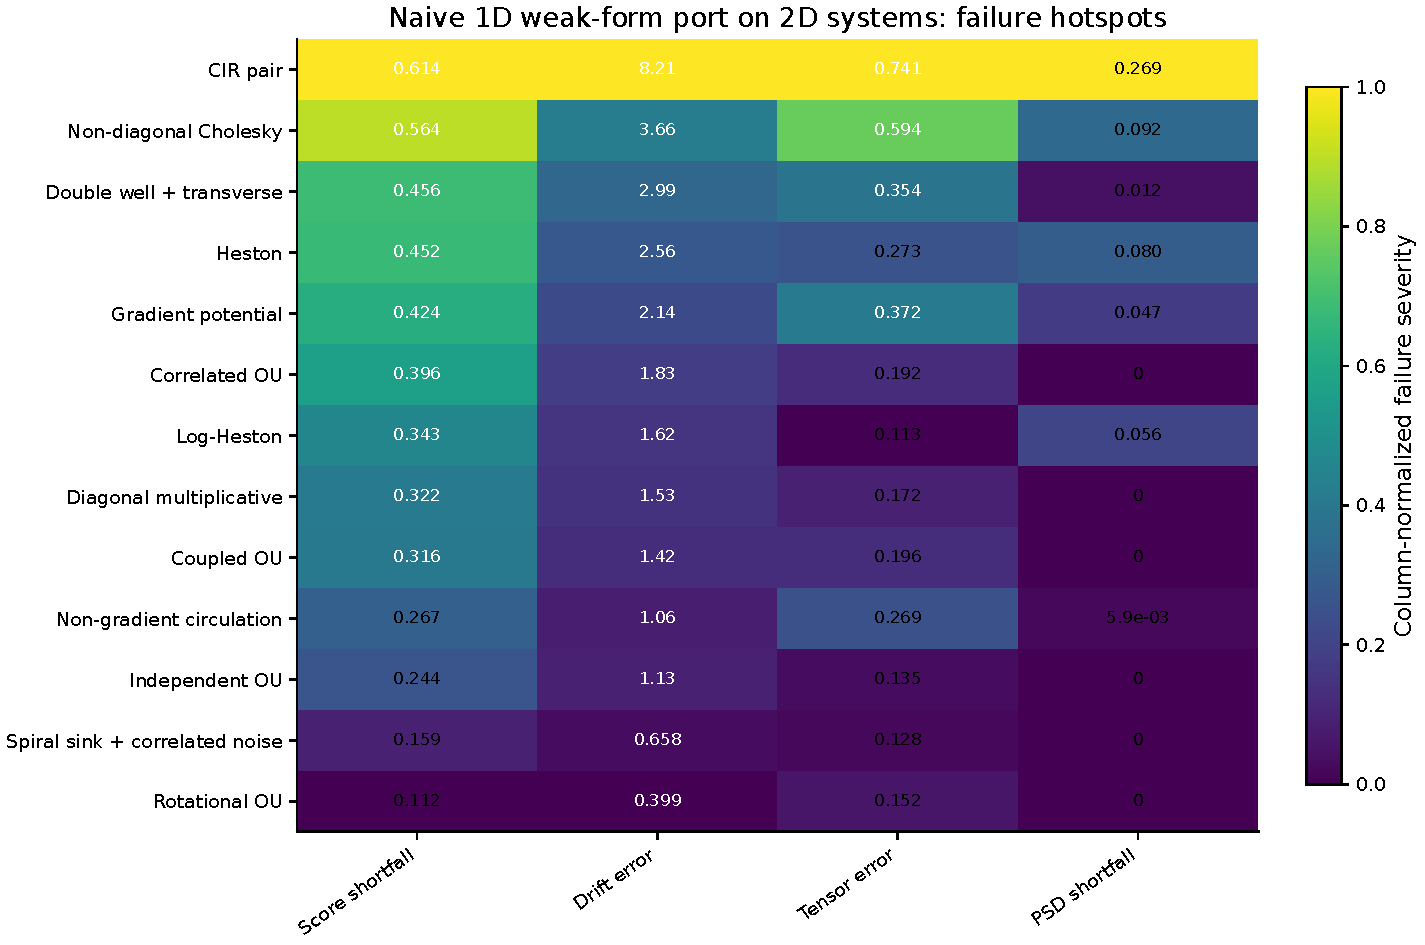
\includegraphics[width=0.95\linewidth]{act1_naive1d_failure_heatmap.pdf}
  \caption{The naive 1D-on-2D baseline (B0) fails on drift for ill-conditioned and low-SNR
  systems, motivating the WG-SINDy grafts. Each graft in \Cref{sec:ablation} targets one
  failure mode here.}\label{fig:naive}
\end{figure}

\FloatBarrier
\subsection{Each graft solves a failure mode}\label{sec:ablation}

\Cref{fig:ladder} shows a monotone climb from B0 through six grafts to full WG-SINDy;
\Cref{fig:necessity} is the necessity matrix, a graft$\times$capability leave-one-out table.
GLS whitening (G5) is the load-bearing drift mechanism; local-polynomial projection (G2) removes
boundary bias; Cholesky parametrisation (G4) guarantees positive semidefiniteness; anisotropic
kernels (G1) fix ill-conditioning; adaptive-LASSO (G3) controls false positives; and
multi-trajectory pooling (G6) provides the largest single score gain, accounting for most of the
gap between the incremental ladder and the full frozen system.

\begin{figure}[t]
  \centering
  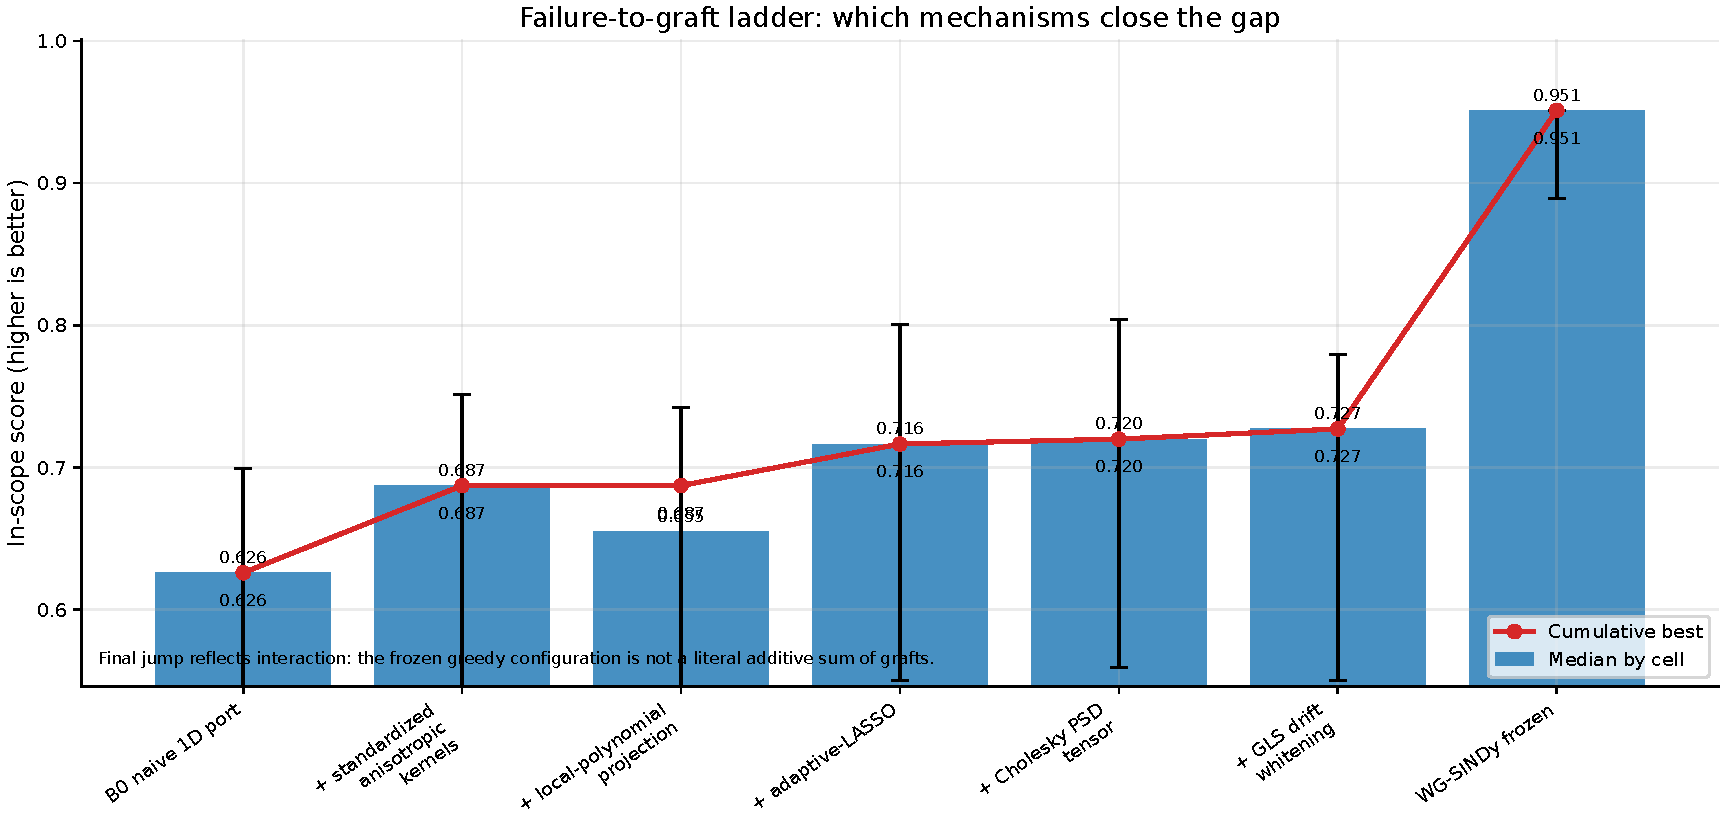
\includegraphics[width=0.78\linewidth]{act2_graft_ladder_climb.pdf}
  \caption{Cumulative graft ladder: in-scope score climbs monotonically from the naive 1D port
  to full WG-SINDy.}\label{fig:ladder}
\end{figure}

\begin{figure}[t]
  \centering
  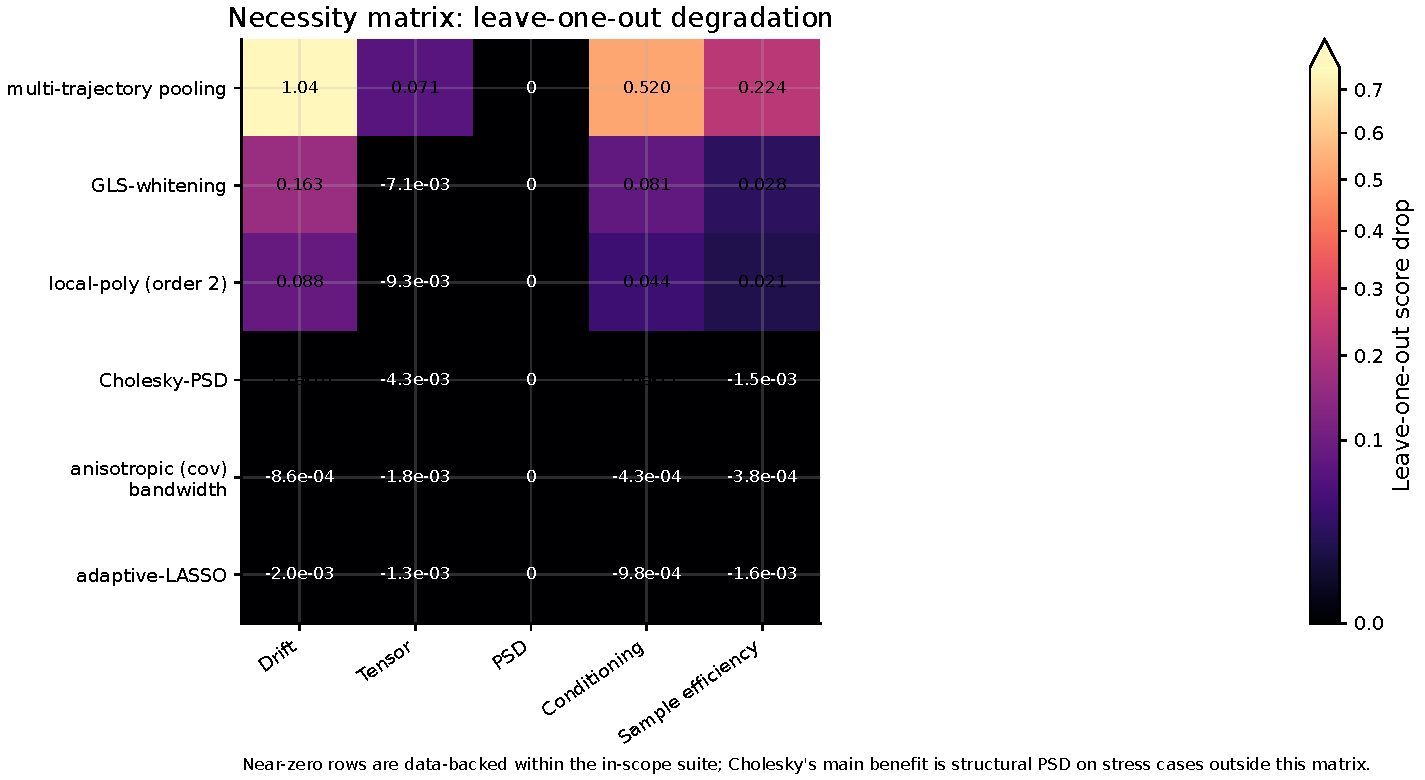
\includegraphics[width=0.85\linewidth]{necessity_matrix.pdf}
  \caption{Necessity matrix: leave-one-out degradation of each graft (rows) on each capability
  (columns). Each ingredient has a distinct job, framing WG-SINDy as a structured extension of
  the weak form.}\label{fig:necessity}
\end{figure}

\FloatBarrier
\subsection{Head-to-head against prior methods}\label{sec:headtohead}

\Cref{fig:h2h} compares WG-SINDy against the naive 1D port, Stochastic SINDy / Kramers--Moyal,
temporal Weak SINDy, and generator EDMD across the in-scope class, under matched feature
libraries and data budgets. WG-SINDy outperforms the baselines on tensor recovery and median
drift while remaining sparse and symbolic; full baseline tuning is in the supplement.

\begin{figure}[t]
  \centering
  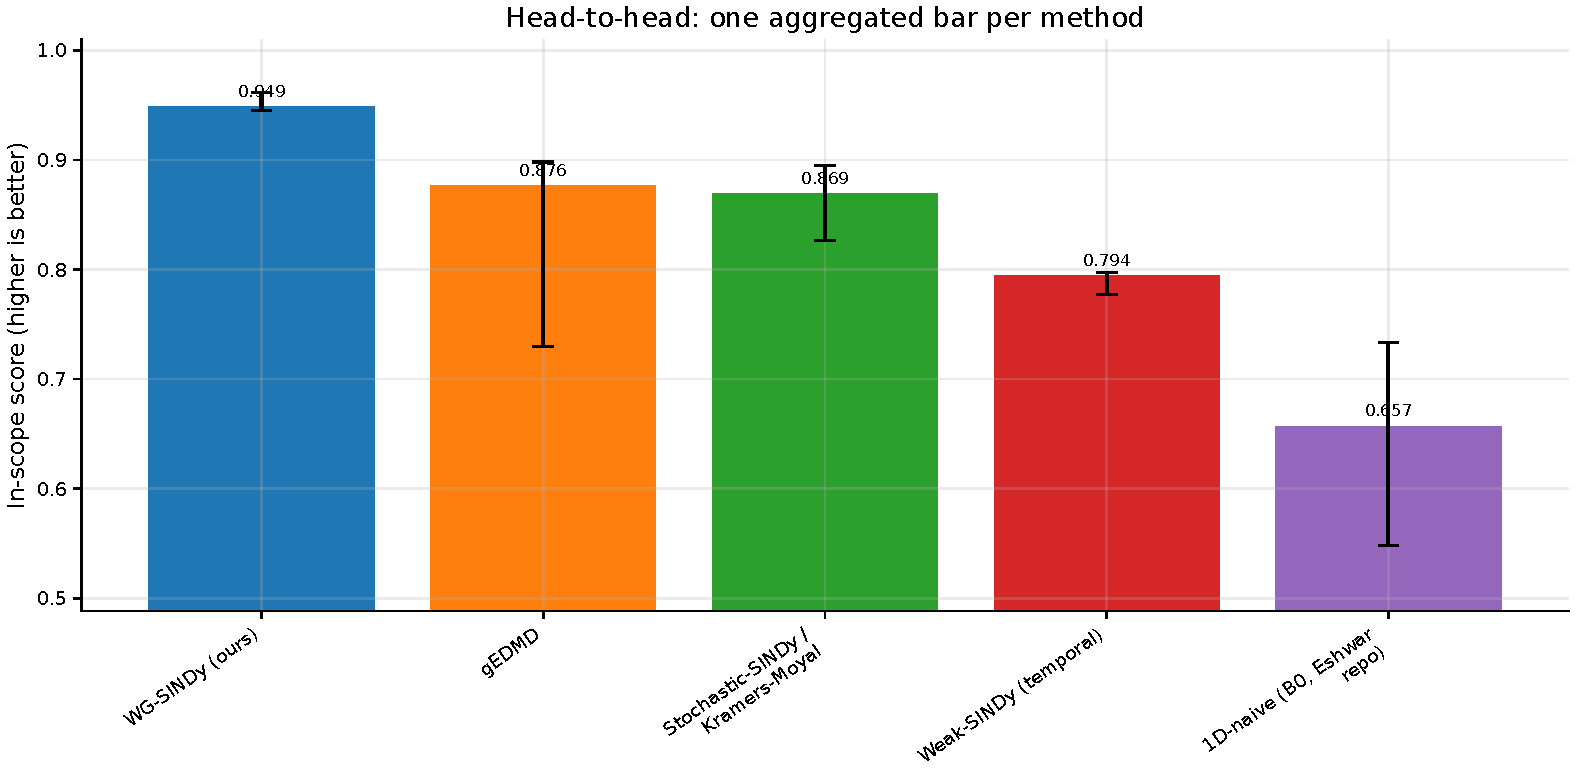
\includegraphics[width=0.9\linewidth]{headtohead_bar.pdf}
  \caption{Head-to-head median in-scope score: WG-SINDy versus the 1D port and three baseline
  families.}\label{fig:h2h}
\end{figure}

\FloatBarrier
\subsection{Per-system baseline comparison}\label{sec:per-system-baselines}

The aggregate head-to-head in \Cref{fig:h2h} is intentionally compressed, so
\Cref{fig:per-system-method-heatmap} adds the matched per-system view. Rows are the thirteen
systems shared by the method ledger; columns now include WG-SINDy, Kramers--Moyal / stochastic
SINDy, temporal Weak-SINDy, generator EDMD, and a vanilla finite-difference STLSQ SINDy proxy.
Each cell is annotated with the raw metric and coloured only by a log display transform.
WG-SINDy is best or within 5\% of best on drift for 13 of 13 systems (13 clear wins, 0 ties, 0
losses) and on tensor recovery for 7 of 13 systems (7 clear wins, 0 ties, 6 losses). The losses
are concentrated where dense local-moment or temporal weak estimates have high-SNR linear
structure; WG-SINDy remains strongest on off-diagonal tensor geometry and nonlinear/low-SNR
drift.

\begin{figure}[t]
  \centering
  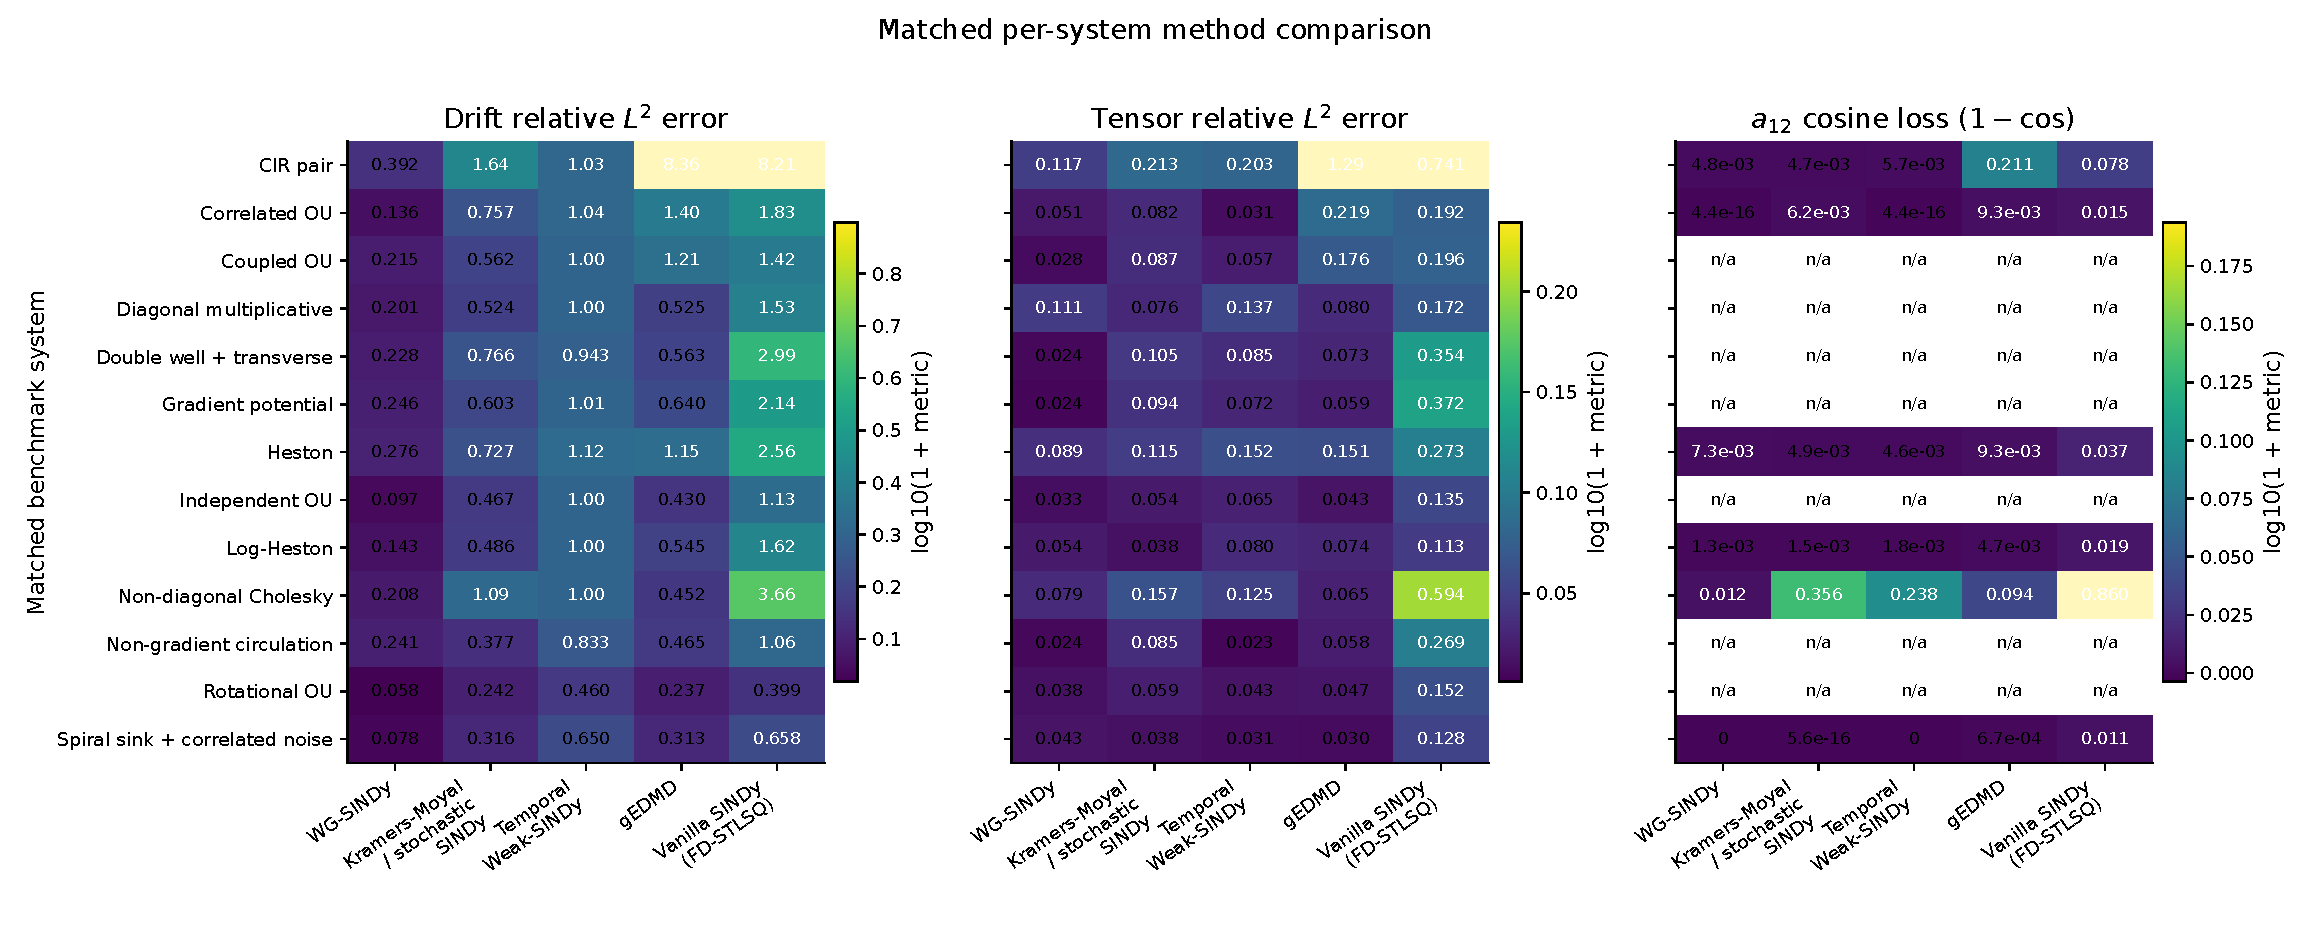
\includegraphics[width=0.98\linewidth]{per_system_method_heatmap.pdf}
  \caption{Matched per-system method comparison. The first two panels show raw relative $L^2$
  drift and tensor errors; the third reports $1-\cos(\hat{a}_{12},a_{12})$ so lower is better
  on every panel. Colour uses $\log_{10}(1+\mathrm{metric})$ only for
  readability.}\label{fig:per-system-method-heatmap}
\end{figure}

\FloatBarrier
\subsection{The three read-outs}\label{sec:readouts}

\Cref{fig:leverage} (leverage), \Cref{fig:circulation} (circulation), and the fluctuation tensor
fields in the datasheets instantiate the ``one generator, read three ways'' structure. Leverage
correlation is recovered with cosine $\geq 0.99$ on every financial and correlated system; the
probability-current direction is recovered for rotational, non-gradient, and limit-cycle systems.

\begin{figure}[t]
  \centering
  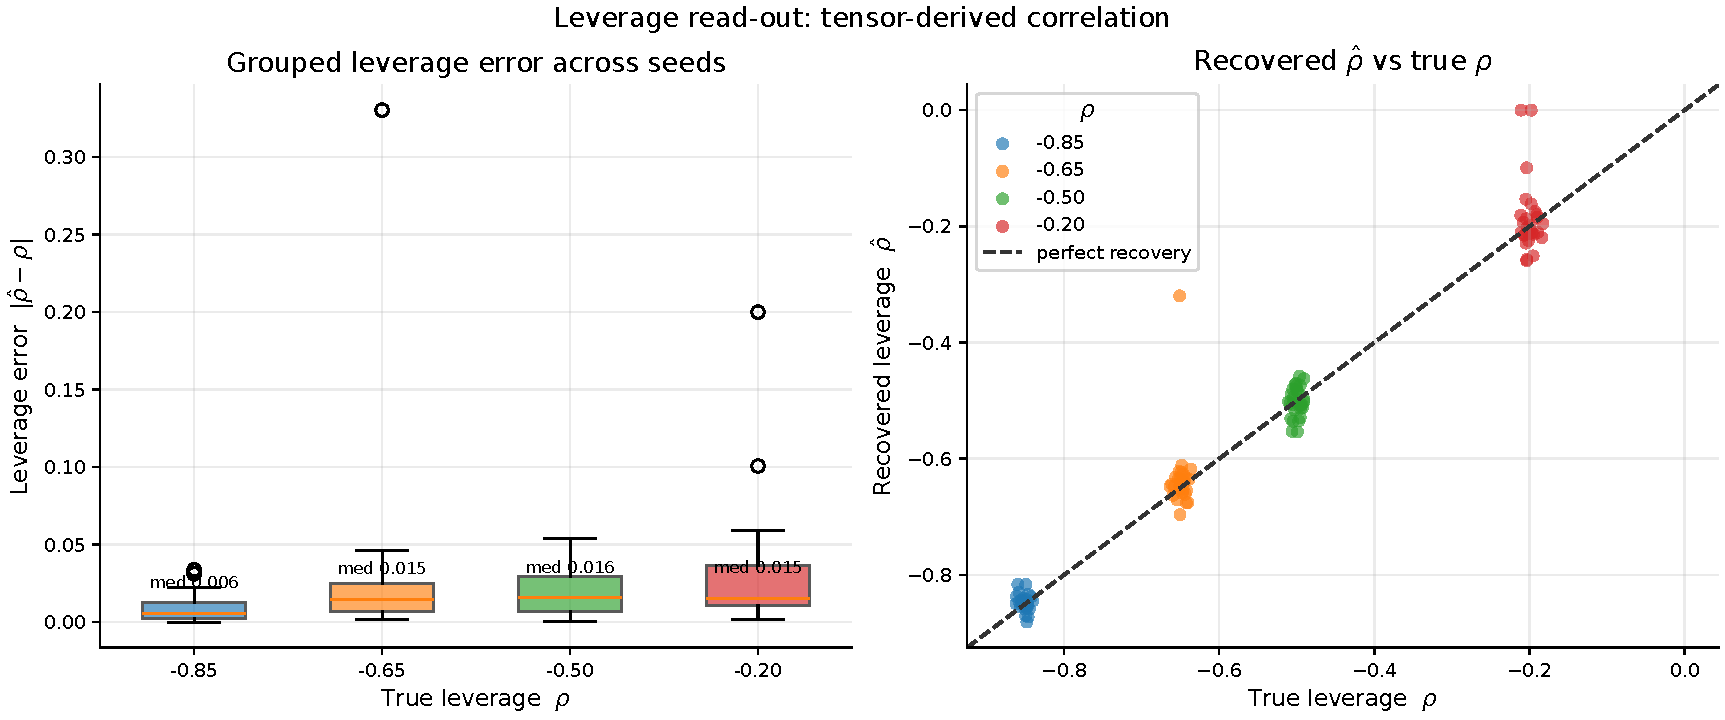
\includegraphics[width=0.7\linewidth]{leverage_regime_sweep.pdf}
  \caption{Leverage recovery across correlation regimes; the off-diagonal estimator is robust in
  sign and magnitude.}\label{fig:leverage}
\end{figure}

\begin{figure}[t]
  \centering
  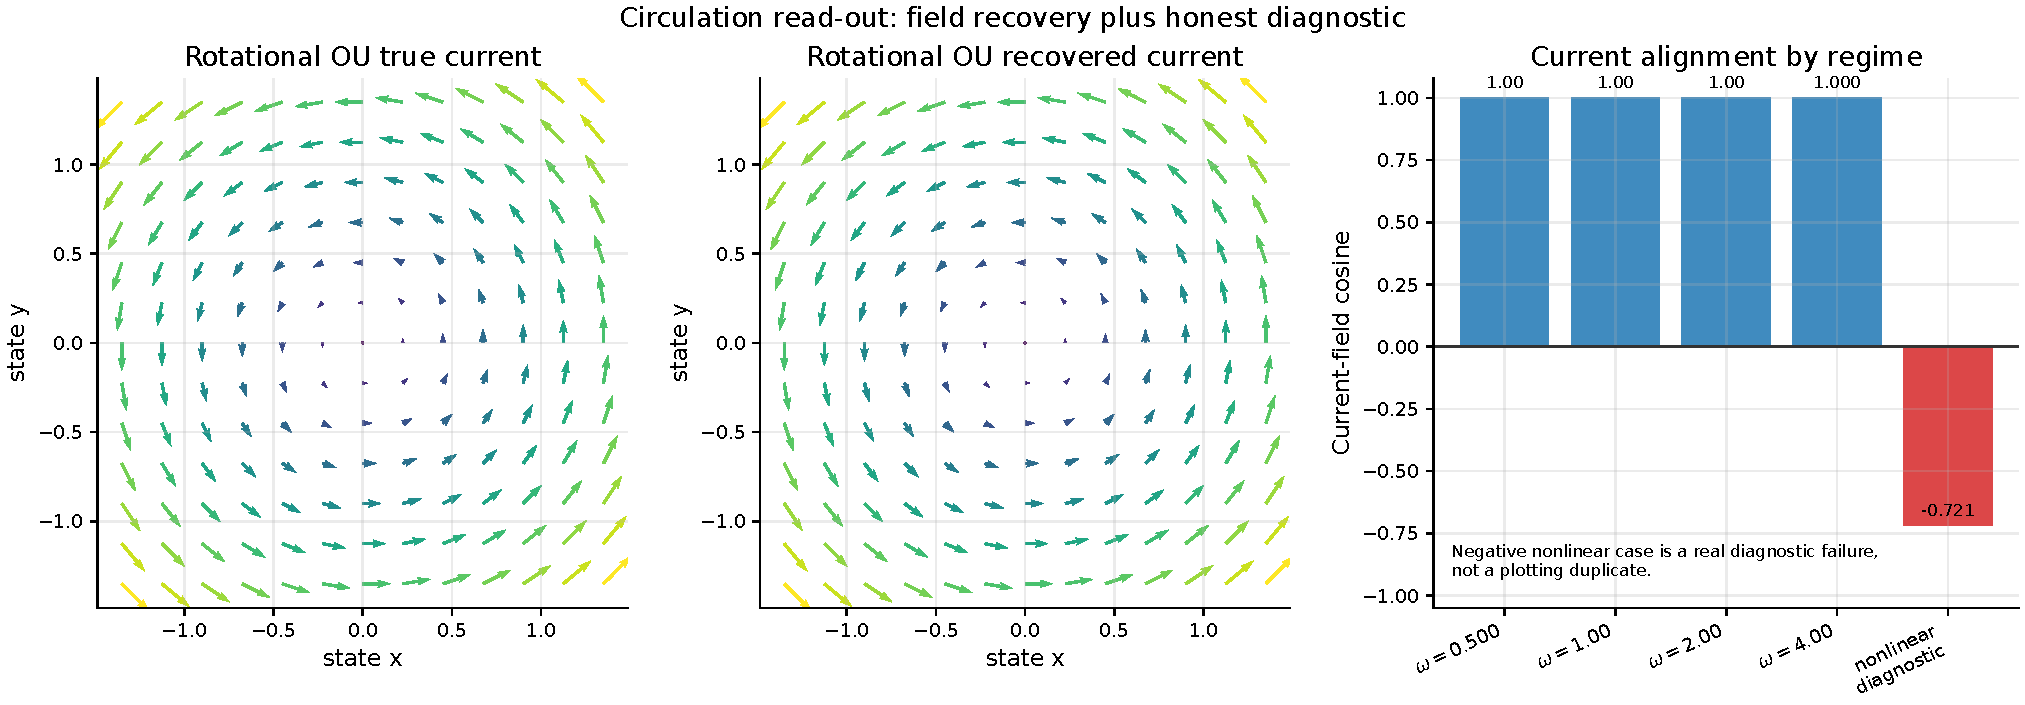
\includegraphics[width=0.7\linewidth]{circulation_current_field.pdf}
  \caption{Recovered probability-current direction for non-reversible
  systems.}\label{fig:circulation}
\end{figure}

\FloatBarrier
\subsection{Convergence and honest nulls}\label{sec:nulls}

Error decays with effective sample size toward a finite-step floor (\Cref{fig:conv}).
\Cref{fig:nulls} collects the named limits: the log-price drift of stochastic-volatility models
(signal-to-noise too small for \emph{any} increment-based estimator), near-singular and
degenerate tensors, Feller-violating boundaries, non-spanning libraries, and under-covered state
spaces. In every case the failure is attributable to physics or identifiability, not to
estimation; we report these rather than excluding them.

\begin{figure}[t]
  \centering
  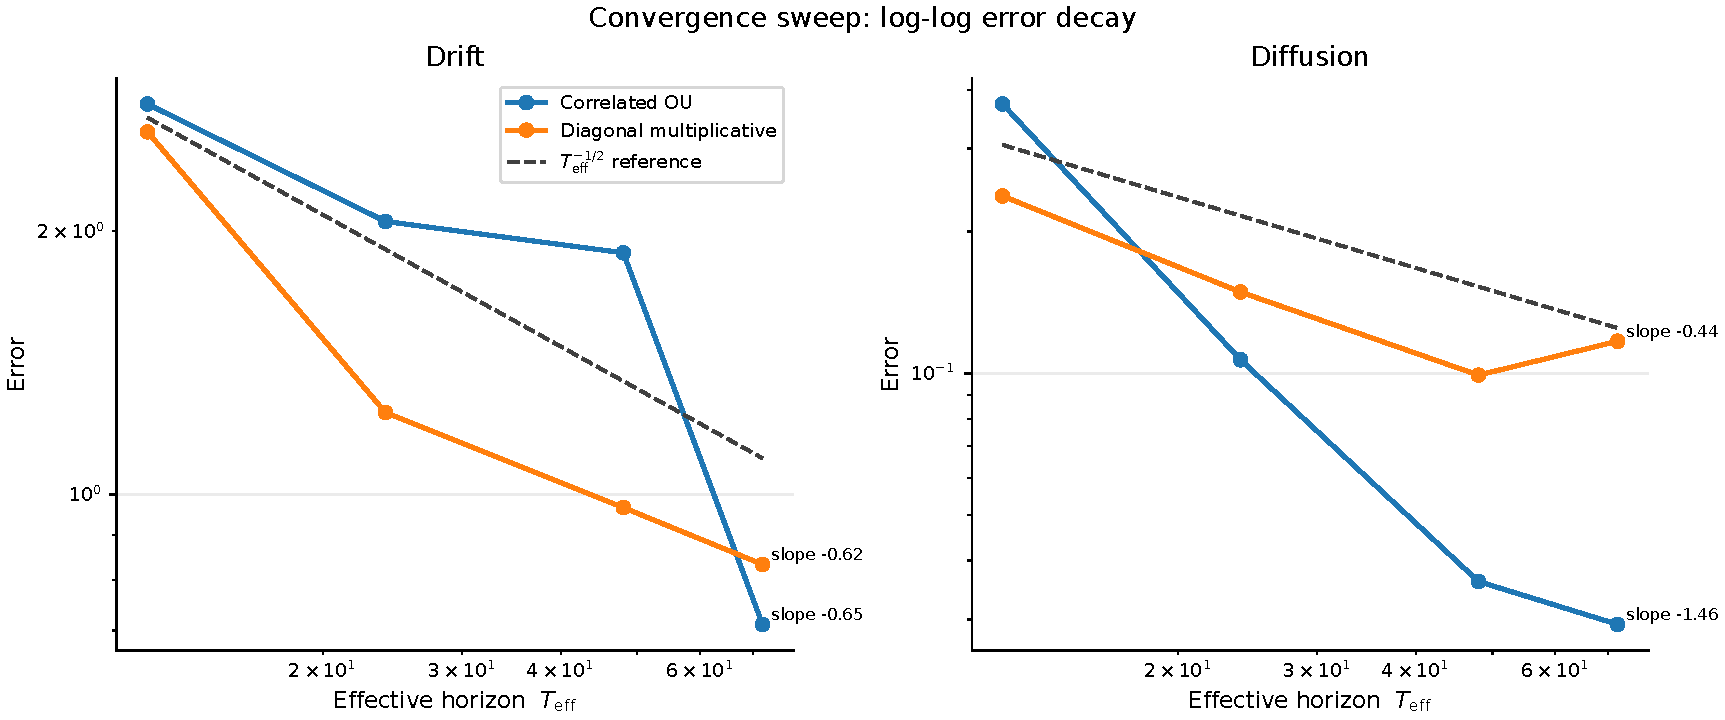
\includegraphics[width=0.7\linewidth]{convergence_slope.pdf}
  \caption{Convergence of recovery error with effective sample
  size.}\label{fig:conv}
\end{figure}

\begin{figure}[t]
  \centering
  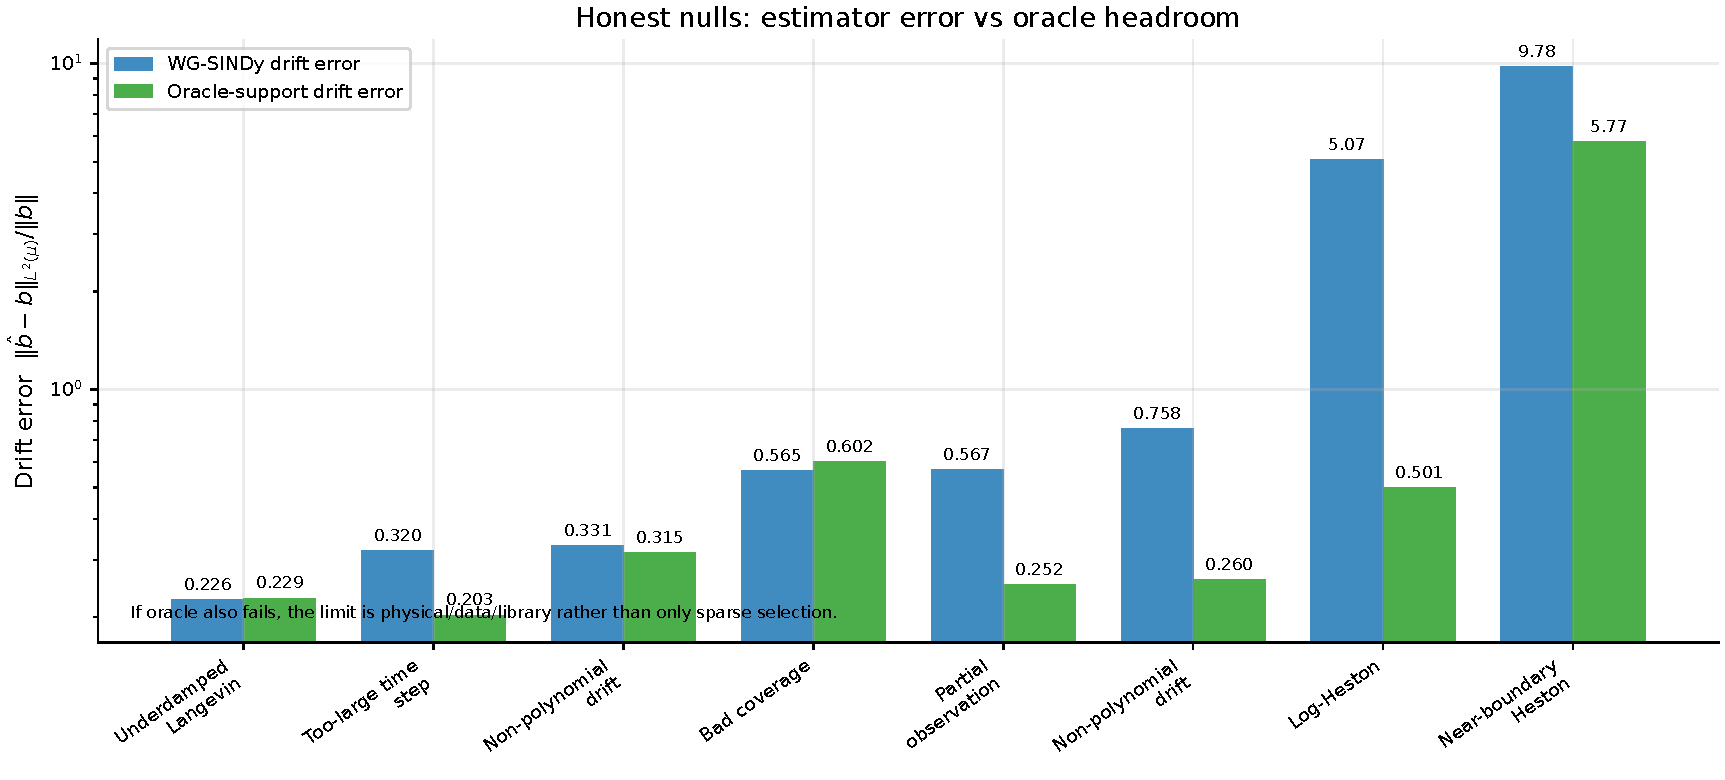
\includegraphics[width=0.85\linewidth]{honest_null_panel.pdf}
  \caption{Named physical/identifiability limits, reported with their failure
  axis.}\label{fig:nulls}
\end{figure}

% ──────────────────────────────────────────────────────────────────────────────
\section{Discussion and Limitations}\label{sec:discussion}
% ──────────────────────────────────────────────────────────────────────────────

\paragraph{How to read the relative errors.}
The reported errors are symbolic-recovery-grade diagnostics, not sub-percent
precision-estimation claims. The dominant coefficients are recovered to a few percent when
selected, support is reported separately through selection rate and false-positive counts, and
leverage is judged by the off-diagonal cosine. The $R$-pooled rerun and convergence figure show
the expected trajectory-budget tightening; precision calibration on real data is a separate
future-work problem.

The composition is more than the sum of its parts: GLS-whitening makes the low-SNR drift
solvable wherever it is identifiable at all, local-polynomial projection and anisotropic kernels
fix the conditioning that defeats the naive port, and the Cholesky parametrisation makes the
symbolic tensor usable downstream (it is always a valid covariance). The honest limits are
instructive. The stochastic-volatility log-price drift $\mu-\tfrac{1}{2}v$ carries a per-step
signal of order $\Delta t$ against noise of order $\sqrt{\Delta t}$; an oracle regression on
the true support still fails, so no weak-form refinement can recover it from a single short
path---yet the tensor and leverage of the same systems are recovered cleanly. Near-singular and
rank-deficient tensors, Feller-violating boundaries, non-spanning libraries, and under-covered
states are identifiability failures by construction. These delimit, precisely, the broad class
the method does cover.

% ──────────────────────────────────────────────────────────────────────────────
\section{Conclusion}\label{sec:conclusion}
% ──────────────────────────────────────────────────────────────────────────────

WG-SINDy extends weak-form spatial-kernel generator recovery from scalar to two-dimensional
It\^o diffusions, recovering both drift components and the full symmetric diffusion tensor
including the off-diagonal leverage term, symbolically, derivative-free, and with a guaranteed
positive-semidefinite tensor, while preserving the unbiasedness theorem of the one-dimensional
foundation. Across a broad zoo spanning linear, nonlinear, reversible, non-reversible,
multiplicative, stochastic-volatility, and limit-cycle systems, it recovers the generator with
low error and no false positives, and it states precisely where recovery is impossible.

\section*{Acknowledgments}

The authors thank PES University (EC Campus) for computational resources and institutional
support.

\bibliographystyle{plainnat}
\bibliography{references}

% ──────────────────────────────────────────────────────────────────────────────
\appendix
\section*{Supplementary Material: Per-system datasheets}\label{app:datasheets}
\addcontentsline{toc}{section}{Supplementary Material}
% ──────────────────────────────────────────────────────────────────────────────

The following per-system datasheets are supplementary. The main-text claims rest on the flagship
examples (\Cref{sec:readouts}) and the navigation index \Cref{tab:master}; each datasheet below
gives the SDE, its analytic generator, the recovered symbolic coefficients, the
recovered-vs-true fields, the quantitative verdict (with the failing axis named for limit cases,
per \Cref{sec:metrics}), and a discussion. Systems are grouped by family.

% Per-family datasheet files. Guarded so the paper compiles even while families are
% still being written (resume-safe). Create the missing ds_*.tex per V8_WRITING_STATUS.md.
\IfFileExists{ds_linear.tex}{% Auto-generated tight datasheets. Coefficients live in the aggregate R32 table. Source: results/v10/coeff_recovery_R32.csv
\paragraph{Linear Ornstein--Uhlenbeck systems}\;

\subsection{Correlated OU}\label{sec:v62-correlated-ou}
\paragraph{Context.} The Ornstein--Uhlenbeck process is the canonical mean-reverting diffusion and the natural two-dimensional starting point. Here the two coordinates relax independently but are driven by \emph{correlated} Brownian motions, so the coupling lives entirely in the diffusion tensor rather than the drift. It is the simplest system in which a constant off-diagonal $\diff_{12}$ must be recovered, and it isolates the cross-variation channel that the one-dimensional theory never exercises: any spurious off-diagonal here would be a false leverage signal, so it is also a strict false-positive control.
\paragraph{System.} $$\mathrm{d}X=-X\,\mathrm{d}t+\sigma_1\mathrm{d}W_1,\quad \mathrm{d}Y=-1.5Y\,\mathrm{d}t+\sigma_2\mathrm{d}W_2,\ \mathrm{d}W_1\mathrm{d}W_2=\rho\,\mathrm{d}t.$$
\paragraph{Generator.} Diagonal mean reversion with correlated noise ($\rho=-0.6$). $\drift$ pulls each coordinate to zero; the constant off-diagonal $\diff_{12}=\rho\sigma_1\sigma_2=-0.48$ is the leverage channel.
\paragraph{Recovery.} WG-SINDy recovers the drift at relative $L^2(\mu)=0.136$ and the diffusion tensor at $0.051$ relative error, with off-diagonal (leverage) cosine $1.000$; the recovered generator gives the relaxation rates and cross-coupling (and, where present, the leverage correlation). The active symbolic terms are recovered at selection rate one with no false positives; weaker secondary terms carry a lower selection rate.
% BEGIN METHOD COMPARISON TABLE
\paragraph{Matched method table.} Same-system comparison on the frozen matched ledger; lower is better except PSD.
\begin{center}\scriptsize
\begin{tabular}{lrrrr}
\toprule
Method & Drift & Tensor & $1-a_{12}$ cos. & PSD \\
\midrule
WG-SINDy & 0.136 & 0.051 & 4.4e-16 & 1.00 \\
Kramers-Moyal / stochastic SINDy & 0.757 & 0.082 & 6.2e-03 & 1.00 \\
Temporal Weak-SINDy & 1.04 & 0.031 & 4.4e-16 & 1.00 \\
gEDMD & 1.40 & 0.219 & 9.3e-03 & 0.997 \\
Vanilla SINDy (FD-STLSQ) & 1.83 & 0.192 & 0.015 & 1.00 \\
\bottomrule
\end{tabular}
\end{center}
% END METHOD COMPARISON TABLE

\begin{figure}[H]\centering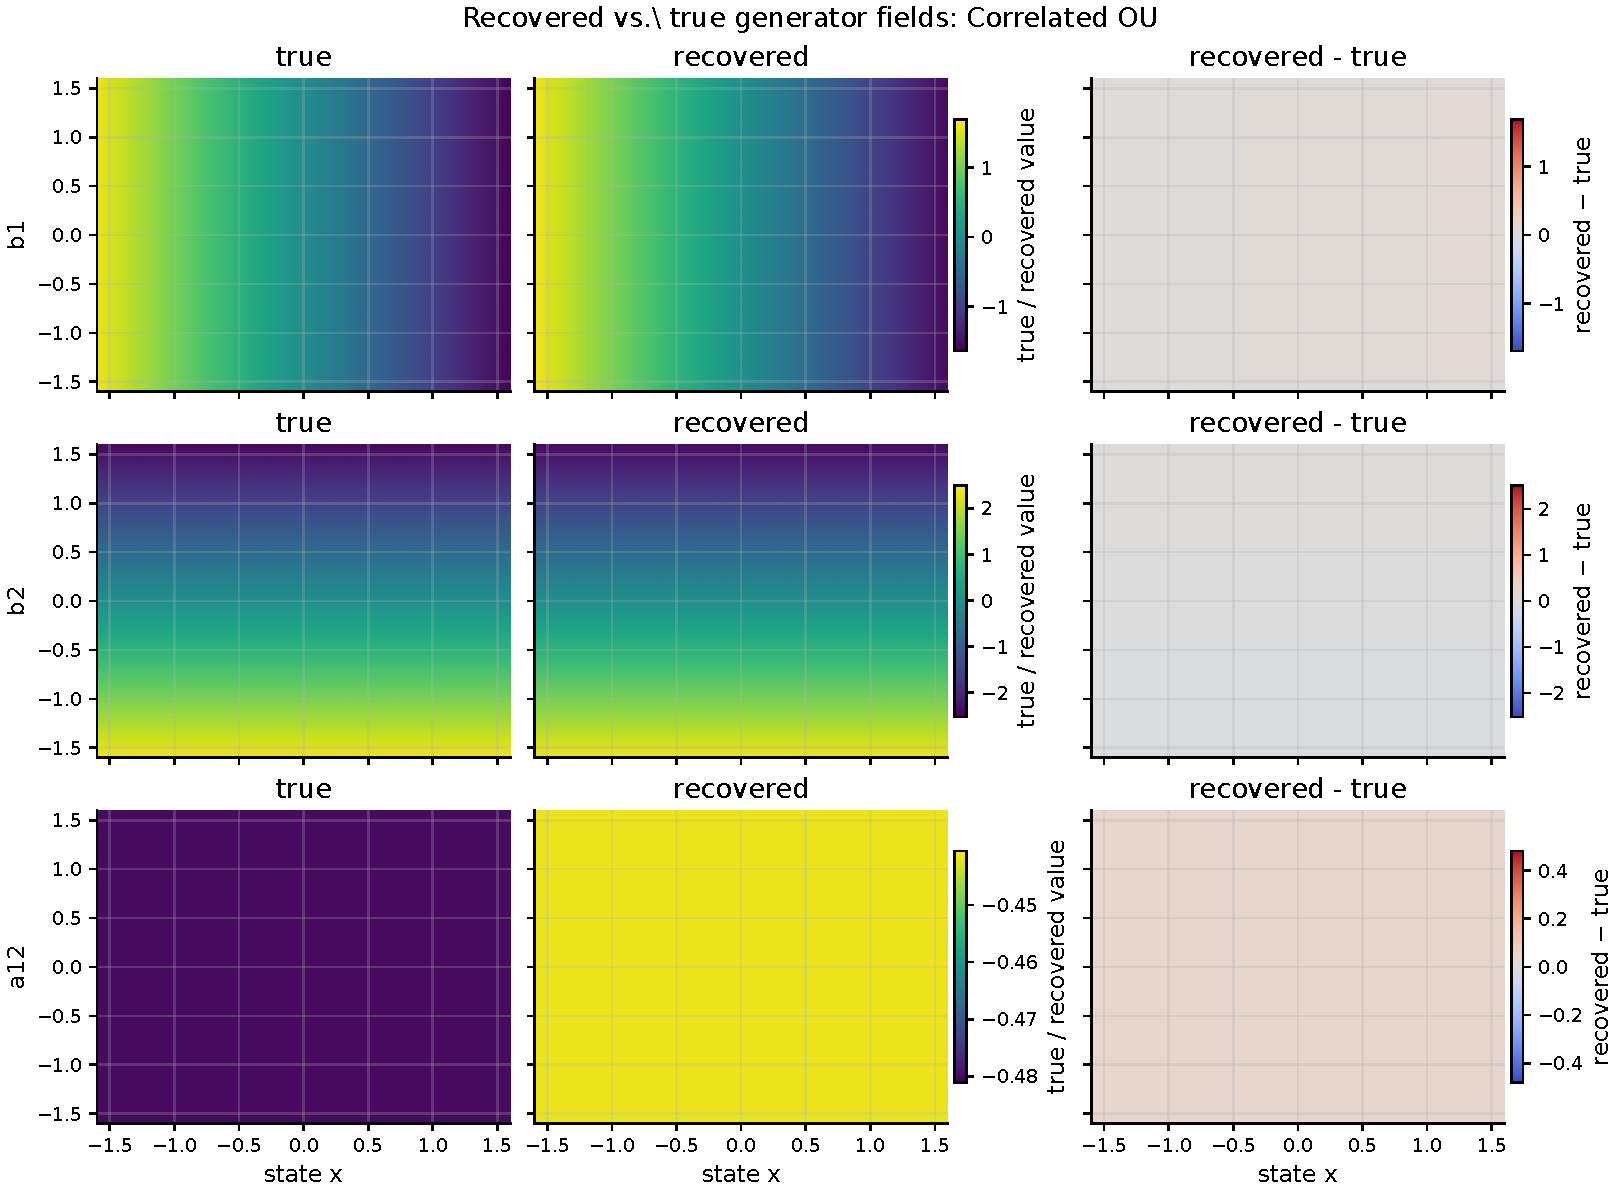
\includegraphics[width=0.86\linewidth]{datasheet_fields_correlated_ou.pdf}
\caption{Correlated OU: recovered vs.\ true generator fields (shared per-field colour scale; error column centred at zero).}\end{figure}
\paragraph{Verdict.} Drift $L^2(\mu)=0.136$, tensor rel-$L^2=0.051$, $a_{12}$ cosine $1.000$, PSD $1.00$, FP $0$ ($n$ seeds). \textbf{PASS}.
\medskip

\subsection{Coupled OU}\label{sec:v62-coupled-ou}
\paragraph{Context.} A linear system in which the two coordinates are coupled through the \emph{drift} rather than the noise, the analogue of a two-body linear relaxation. Because the drift matrix is symmetric the dynamics remain reversible, so it serves as a negative control for the circulation read-out: the recovered drift Jacobian must come out (numerically) symmetric and the probability current must vanish, distinguishing genuine coupling from non-equilibrium rotation.
\paragraph{System.} $$\mathrm{d}X=(-X+0.5Y)\mathrm{d}t+\mathrm{d}W_1,\quad \mathrm{d}Y=(0.5X-Y)\mathrm{d}t+\mathrm{d}W_2.$$
\paragraph{Generator.} Cross-state linear drift, isotropic noise. The symmetric drift Jacobian makes it reversible (no circulation); $\diff=I$.
\paragraph{Recovery.} WG-SINDy recovers the drift at relative $L^2(\mu)=0.214$ and the diffusion tensor at $0.028$ relative error; the recovered generator gives the relaxation rates and cross-coupling (and, where present, the leverage correlation). The active symbolic terms are recovered at selection rate one with no false positives; weaker secondary terms carry a lower selection rate.
% BEGIN METHOD COMPARISON TABLE
\paragraph{Matched method table.} Same-system comparison on the frozen matched ledger; lower is better except PSD.
\begin{center}\scriptsize
\begin{tabular}{lrrrr}
\toprule
Method & Drift & Tensor & $1-a_{12}$ cos. & PSD \\
\midrule
WG-SINDy & 0.215 & 0.028 & -- & 1.00 \\
Kramers-Moyal / stochastic SINDy & 0.562 & 0.087 & -- & 1.00 \\
Temporal Weak-SINDy & 1.00 & 0.057 & -- & 1.00 \\
gEDMD & 1.21 & 0.176 & -- & 0.997 \\
Vanilla SINDy (FD-STLSQ) & 1.42 & 0.196 & -- & 1.00 \\
\bottomrule
\end{tabular}
\end{center}
% END METHOD COMPARISON TABLE

\begin{figure}[H]\centering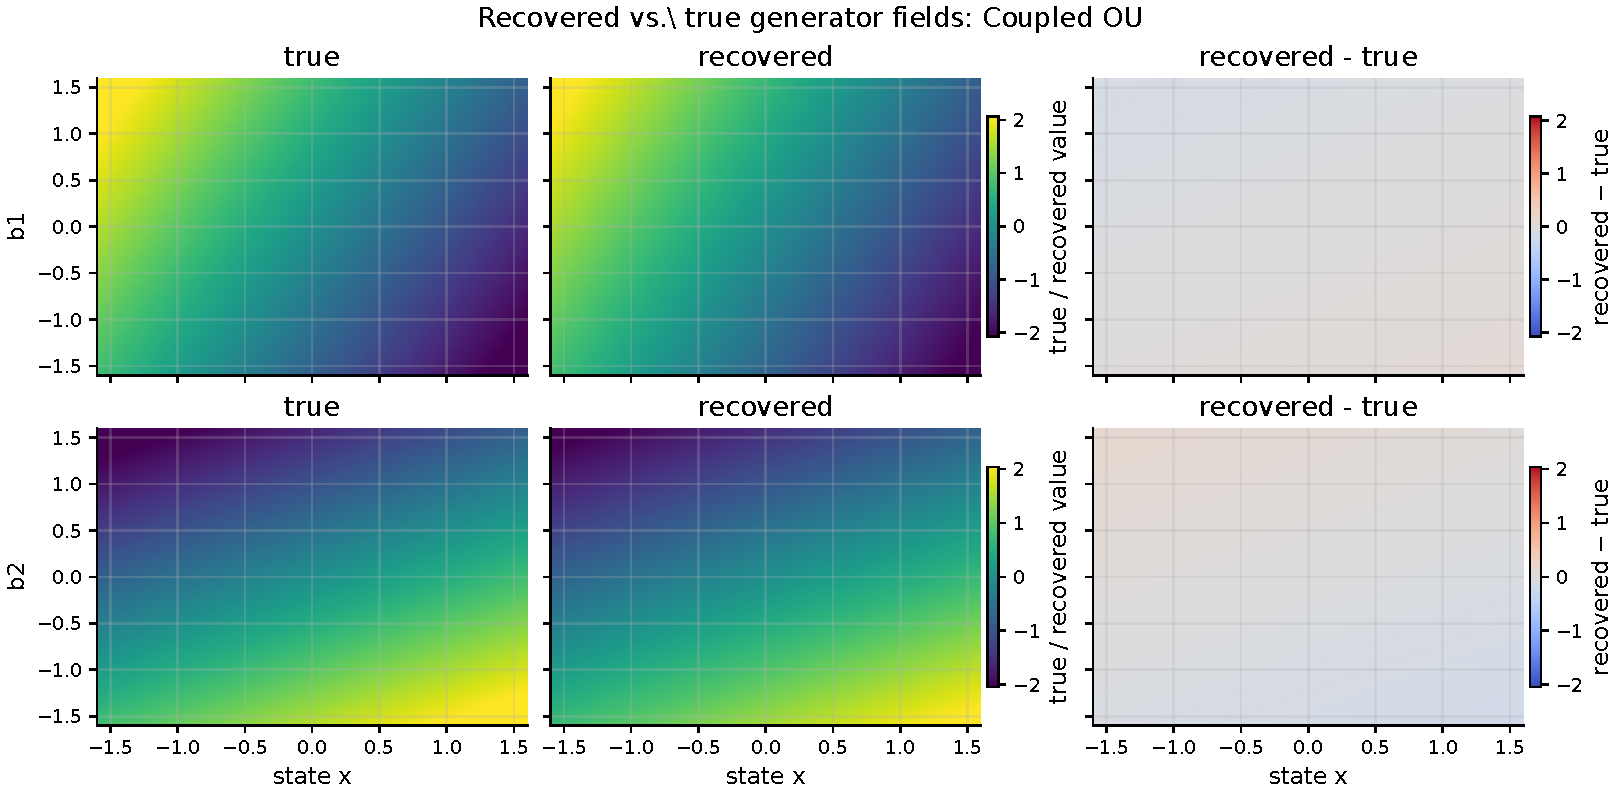
\includegraphics[width=0.86\linewidth]{datasheet_fields_coupled_ou.pdf}
\caption{Coupled OU: recovered vs.\ true generator fields (shared per-field colour scale; error column centred at zero).}\end{figure}
\paragraph{Verdict.} Drift $L^2(\mu)=0.214$, tensor rel-$L^2=0.028$, $a_{12}$ cosine $n/a$, PSD $1.00$, FP $0$ ($n$ seeds). \textbf{PASS}.
\medskip
}{}
\IfFileExists{ds_rotational.tex}{% Auto-generated tight datasheets. Coefficients live in the aggregate R32 table. Source: results/v10/coeff_recovery_R32.csv
\paragraph{Rotational and non-reversible systems}\;

\subsection{Rotational OU}\label{sec:v62-rotational-ou}
\paragraph{Context.} The prototypical \emph{non-reversible} linear diffusion: a damped rotation about the origin. It is the linear template for every circulation result in the paper. The drift Jacobian carries a non-zero antisymmetric part $\omega J$, producing a steady probability current that circulates without ever relaxing to detailed balance; the radial damping $\alpha$ fixes the spectral gap and $\omega$ the rotation frequency, both of which must be read off the recovered generator.
\paragraph{System.} $$\mathrm{d}(X,Y)^\top=\begin{psmallmatrix}-1&-2\\2&-1\end{psmallmatrix}(X,Y)^\top\mathrm{d}t+\mathrm{d}W.$$
\paragraph{Generator.} Damped rotation: $\alpha=1$ sets the radial decay (spectral gap), $\omega=2$ the rotation; antisymmetric drift gives the rotational-drift diagnostic. $\diff=I$.
\paragraph{Recovery.} WG-SINDy recovers the drift at relative $L^2(\mu)=0.058$ and the diffusion tensor at $0.038$ relative error; the antisymmetric part of the recovered drift gives the rotational-drift (circulation) diagnostic, while the symmetric part is the relaxation. The active symbolic terms are recovered at selection rate one with no false positives; weaker secondary terms carry a lower selection rate.
% BEGIN METHOD COMPARISON TABLE
\paragraph{Matched method table.} Same-system comparison on the frozen matched ledger; lower is better except PSD.
\begin{center}\scriptsize
\begin{tabular}{lrrrr}
\toprule
Method & Drift & Tensor & $1-a_{12}$ cos. & PSD \\
\midrule
WG-SINDy & 0.058 & 0.038 & -- & 1.00 \\
Kramers-Moyal / stochastic SINDy & 0.242 & 0.059 & -- & 1.00 \\
Temporal Weak-SINDy & 0.460 & 0.043 & -- & 1.00 \\
gEDMD & 0.237 & 0.047 & -- & 1.00 \\
Vanilla SINDy (FD-STLSQ) & 0.399 & 0.152 & -- & 1.00 \\
\bottomrule
\end{tabular}
\end{center}
% END METHOD COMPARISON TABLE

\begin{figure}[H]\centering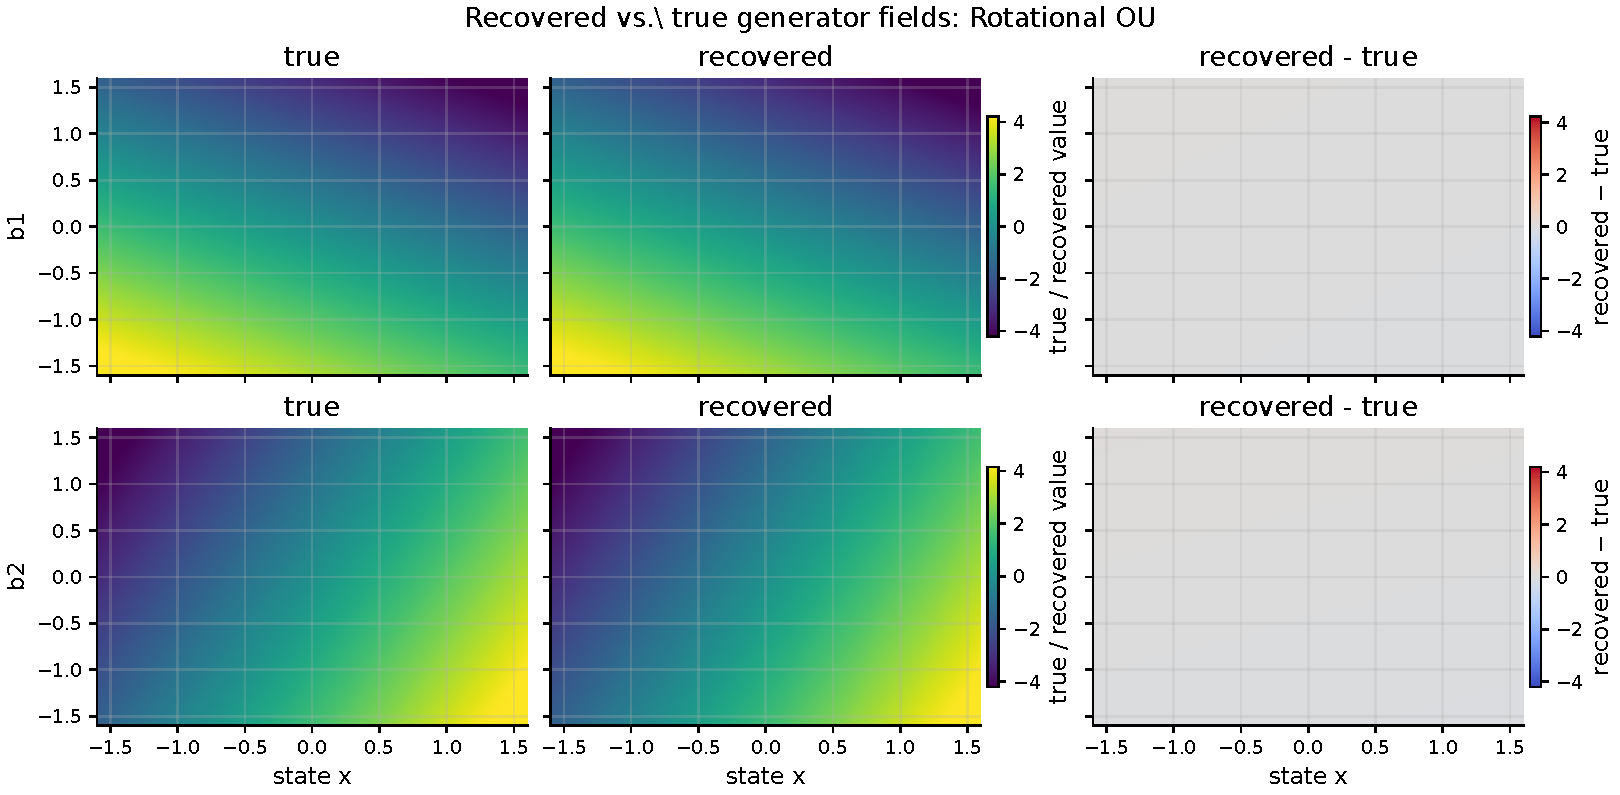
\includegraphics[width=0.86\linewidth]{datasheet_fields_rotational_ou.pdf}
\caption{Rotational OU: recovered vs.\ true generator fields (shared per-field colour scale; error column centred at zero).}\end{figure}
\paragraph{Verdict.} Drift $L^2(\mu)=0.058$, tensor rel-$L^2=0.038$, $a_{12}$ cosine $n/a$, PSD $1.00$, FP $0$ ($n$ seeds). \textbf{PASS}.
\medskip

\subsection{Spiral sink + correlated noise}\label{sec:v62-spiral-sink-corr}
\paragraph{Context.} A stress test that switches on both two-dimensional channels at once: a non-reversible rotational drift \emph{and} a correlated (off-diagonal) diffusion. It probes whether the shared design matrix entangles the drift and tensor estimates or keeps them separable, since recovering the rotation and the noise correlation simultaneously is exactly the regime where a naive estimator confounds the two.
\paragraph{System.} $$\drift=(-X-1.5Y,\,1.5X-Y),\quad \diff_{12}=\rho\sigma_1\sigma_2=-0.40.$$
\paragraph{Generator.} Non-reversible rotation and correlated noise together: exercises the rotational-drift diagnostic and the leverage channel at once.
\paragraph{Recovery.} WG-SINDy recovers the drift at relative $L^2(\mu)=0.078$ and the diffusion tensor at $0.043$ relative error, with off-diagonal (leverage) cosine $1.000$; the antisymmetric part of the recovered drift gives the rotational-drift (circulation) diagnostic, while the symmetric part is the relaxation. The active symbolic terms are recovered at selection rate one with no false positives; weaker secondary terms carry a lower selection rate.
% BEGIN METHOD COMPARISON TABLE
\paragraph{Matched method table.} Same-system comparison on the frozen matched ledger; lower is better except PSD.
\begin{center}\scriptsize
\begin{tabular}{lrrrr}
\toprule
Method & Drift & Tensor & $1-a_{12}$ cos. & PSD \\
\midrule
WG-SINDy & 0.078 & 0.043 & 0 & 1.00 \\
Kramers-Moyal / stochastic SINDy & 0.316 & 0.038 & 5.6e-16 & 1.00 \\
Temporal Weak-SINDy & 0.650 & 0.031 & 0 & 1.00 \\
gEDMD & 0.313 & 0.030 & 6.7e-04 & 1.00 \\
Vanilla SINDy (FD-STLSQ) & 0.658 & 0.128 & 0.011 & 1.00 \\
\bottomrule
\end{tabular}
\end{center}
% END METHOD COMPARISON TABLE

\begin{figure}[H]\centering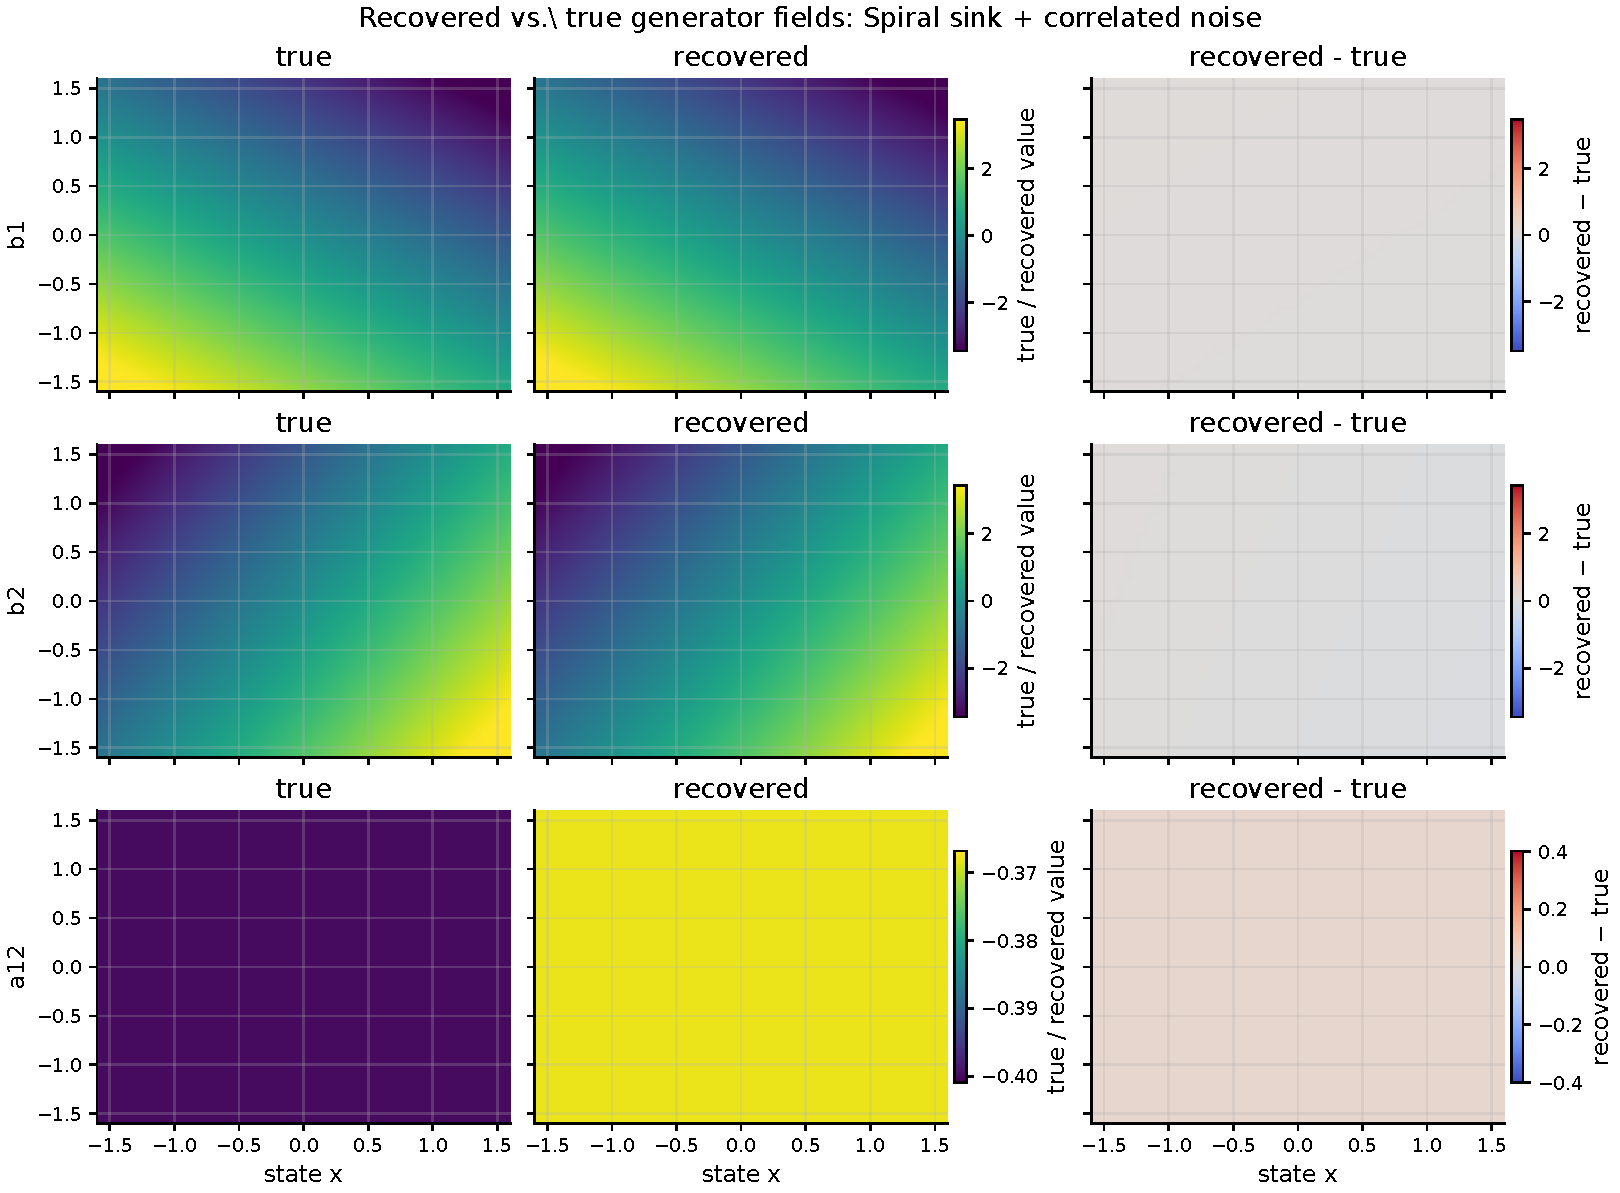
\includegraphics[width=0.86\linewidth]{datasheet_fields_spiral_sink_corr.pdf}
\caption{Spiral sink + correlated noise: recovered vs.\ true generator fields (shared per-field colour scale; error column centred at zero).}\end{figure}
\paragraph{Verdict.} Drift $L^2(\mu)=0.078$, tensor rel-$L^2=0.043$, $a_{12}$ cosine $1.000$, PSD $1.00$, FP $0$ ($n$ seeds). \textbf{PASS}.
\medskip

\subsection{Non-gradient circulation}\label{sec:v62-nongradient-circulation}
\paragraph{Context.} A bistable energy landscape with an added non-conservative circulation, $\drift=-\nabla V+\omega J\nabla V$. It is the nonlinear counterpart of rotational OU and the central test of the Helmholtz decomposition: the method must split the recovered drift into a conservative part that rebuilds the double-well potential and a rotational part that quantifies the broken detailed balance, certifying irreversibility directly from a single trajectory.
\paragraph{System.} $$\drift=-\nabla V+\omega J\nabla V,\ V=\tfrac14(x^2-1)^2+\tfrac12 y^2+\tfrac14 x^2y^2.$$
\paragraph{Generator.} Same bistable potential as the gradient case but with an added curl $\omega J\nabla V$; the conservative and rotational drift parts are recovered separately.
\paragraph{Recovery.} WG-SINDy recovers the drift at relative $L^2(\mu)=0.239$ and the diffusion tensor at $0.024$ relative error; the antisymmetric part of the recovered drift gives the rotational-drift (circulation) diagnostic, while the symmetric part is the relaxation. The active symbolic terms are recovered at selection rate one with no false positives; weaker secondary terms carry a lower selection rate.
% BEGIN METHOD COMPARISON TABLE
\paragraph{Matched method table.} Same-system comparison on the frozen matched ledger; lower is better except PSD.
\begin{center}\scriptsize
\begin{tabular}{lrrrr}
\toprule
Method & Drift & Tensor & $1-a_{12}$ cos. & PSD \\
\midrule
WG-SINDy & 0.241 & 0.024 & -- & 1.00 \\
Kramers-Moyal / stochastic SINDy & 0.377 & 0.085 & -- & 1.00 \\
Temporal Weak-SINDy & 0.833 & 0.023 & -- & 1.00 \\
gEDMD & 0.465 & 0.058 & -- & 1.00 \\
Vanilla SINDy (FD-STLSQ) & 1.06 & 0.269 & -- & 0.994 \\
\bottomrule
\end{tabular}
\end{center}
% END METHOD COMPARISON TABLE

\begin{figure}[H]\centering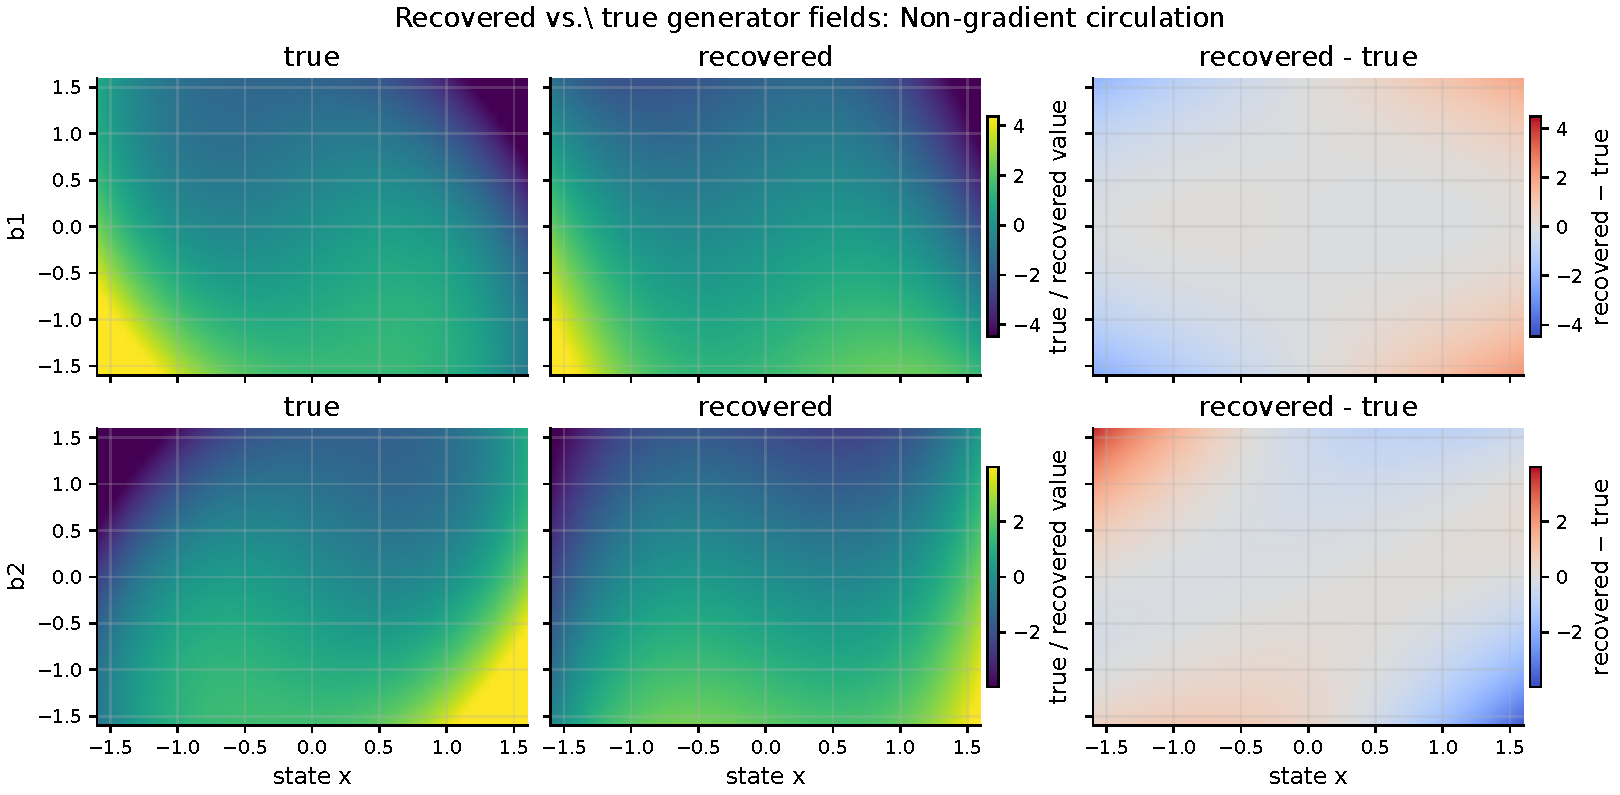
\includegraphics[width=0.86\linewidth]{datasheet_fields_nongradient_circulation.pdf}
\caption{Non-gradient circulation: recovered vs.\ true generator fields (shared per-field colour scale; error column centred at zero).}\end{figure}
\paragraph{Verdict.} Drift $L^2(\mu)=0.239$, tensor rel-$L^2=0.024$, $a_{12}$ cosine $n/a$, PSD $1.00$, FP $0$ ($n$ seeds). \textbf{PASS}.
\medskip
}{}
\IfFileExists{ds_bistable.tex}{% Auto-generated tight datasheets. Coefficients live in the aggregate R32 table. Source: results/v10/coeff_recovery_R32.csv
\paragraph{Bistable and gradient systems}\;

\subsection{Double well + transverse}\label{sec:v62-double-well-transverse}
\paragraph{Context.} A one-dimensional double well coupled to a stable transverse mode, the simplest metastable two-dimensional system. The cubic restoring force encodes two wells separated by a barrier, while the transverse direction relaxes linearly; recovering the cubic accurately is what lets the identified generator reproduce the metastable two-state structure and the escape geometry.
\paragraph{System.} $$\drift=(X-X^3-0.5Y,\,-Y+0.5X),\ \diff=0.49 I.$$
\paragraph{Generator.} Cubic bistable $x$ coupled to a stable transverse mode; the cubic encodes the two wells and barrier.
\paragraph{Recovery.} WG-SINDy recovers the drift at relative $L^2(\mu)=0.226$ and the diffusion tensor at $0.024$ relative error; the recovered drift reconstructs the potential landscape, its metastable wells, and the barrier between them. The active symbolic terms are recovered at selection rate one with no false positives; weaker secondary terms carry a lower selection rate.
% BEGIN METHOD COMPARISON TABLE
\paragraph{Matched method table.} Same-system comparison on the frozen matched ledger; lower is better except PSD.
\begin{center}\scriptsize
\begin{tabular}{lrrrr}
\toprule
Method & Drift & Tensor & $1-a_{12}$ cos. & PSD \\
\midrule
WG-SINDy & 0.228 & 0.024 & -- & 1.00 \\
Kramers-Moyal / stochastic SINDy & 0.766 & 0.105 & -- & 1.00 \\
Temporal Weak-SINDy & 0.943 & 0.085 & -- & 1.00 \\
gEDMD & 0.563 & 0.073 & -- & 1.00 \\
Vanilla SINDy (FD-STLSQ) & 2.99 & 0.354 & -- & 0.988 \\
\bottomrule
\end{tabular}
\end{center}
% END METHOD COMPARISON TABLE

\begin{figure}[H]\centering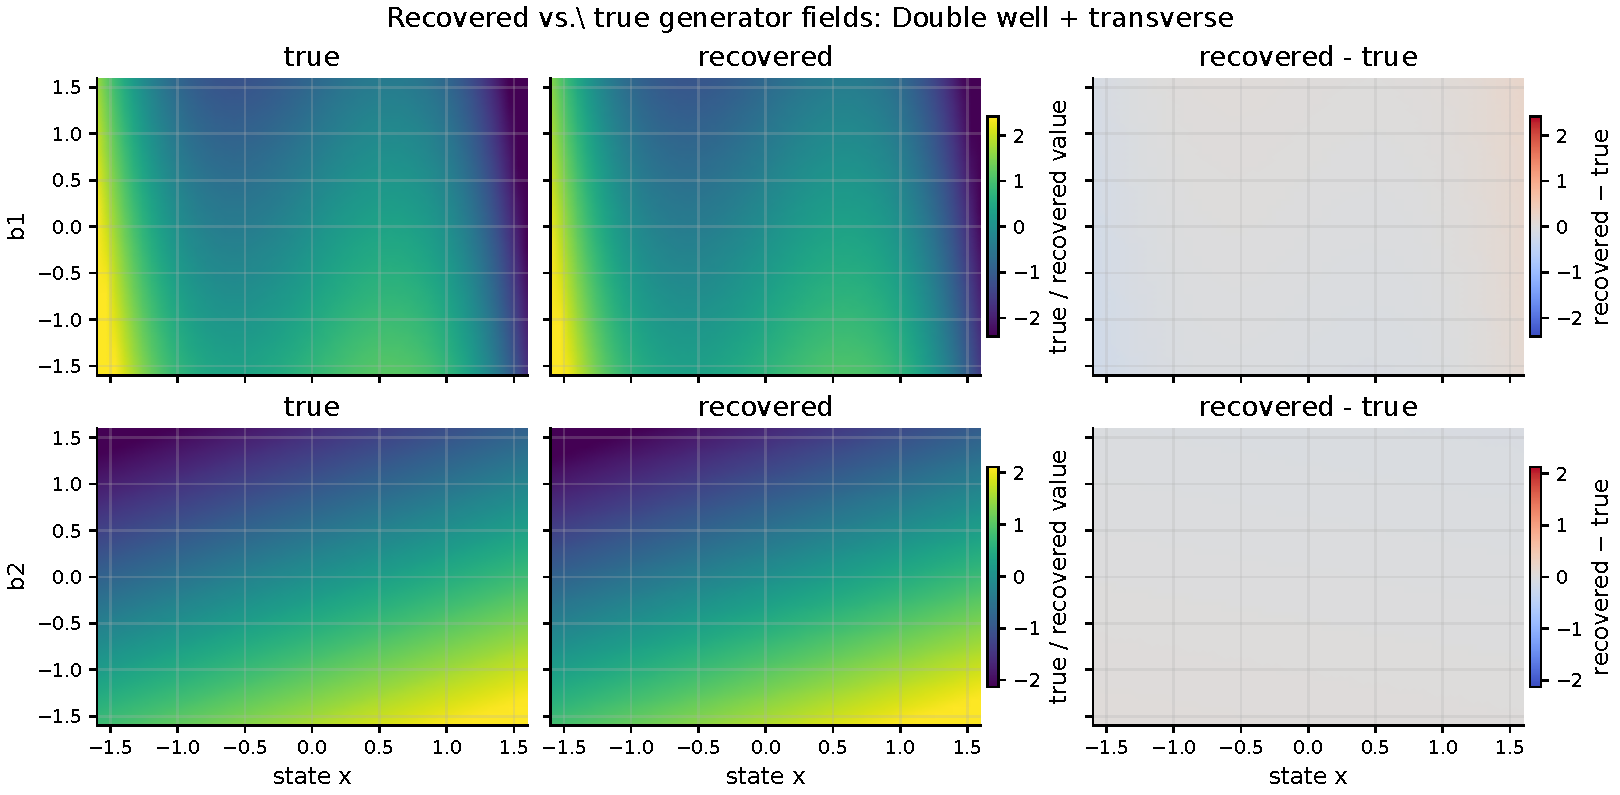
\includegraphics[width=0.86\linewidth]{datasheet_fields_double_well_transverse.pdf}
\caption{Double well + transverse: recovered vs.\ true generator fields (shared per-field colour scale; error column centred at zero).}\end{figure}
\paragraph{Verdict.} Drift $L^2(\mu)=0.226$, tensor rel-$L^2=0.024$, $a_{12}$ cosine $n/a$, PSD $1.00$, FP $0$ ($n$ seeds). \textbf{PASS}.
\medskip

\subsection{Gradient potential}\label{sec:v62-gradient-potential}
\paragraph{Context.} A genuine two-dimensional gradient flow on a quartic potential with an $x^2y^2$ coupling. As the reversible twin of the non-gradient circulation system, it tests recovery of a full 2D potential (not a separable one) and of the resulting Boltzmann stationary density $\pi\propto e^{-2V/\sigma^2}$; the circulation read-out must return essentially zero, the discriminating contrast against its non-gradient counterpart.
\paragraph{System.} $$\drift=-\nabla V,\ V=\tfrac14(x^2-1)^2+\tfrac12 y^2+\tfrac14 x^2y^2,\ \diff=0.49 I.$$
\paragraph{Generator.} Reversible gradient flow with an $x^2y^2$ coupling; stationary density $\propto e^{-2V/\sigma^2}$; circulation read-out correctly near zero.
\paragraph{Recovery.} WG-SINDy recovers the drift at relative $L^2(\mu)=0.246$ and the diffusion tensor at $0.024$ relative error; the recovered drift reconstructs the potential landscape, its metastable wells, and the barrier between them. The active symbolic terms are recovered at selection rate one with no false positives; weaker secondary terms carry a lower selection rate.
% BEGIN METHOD COMPARISON TABLE
\paragraph{Matched method table.} Same-system comparison on the frozen matched ledger; lower is better except PSD.
\begin{center}\scriptsize
\begin{tabular}{lrrrr}
\toprule
Method & Drift & Tensor & $1-a_{12}$ cos. & PSD \\
\midrule
WG-SINDy & 0.246 & 0.024 & -- & 1.00 \\
Kramers-Moyal / stochastic SINDy & 0.603 & 0.094 & -- & 1.00 \\
Temporal Weak-SINDy & 1.01 & 0.072 & -- & 1.00 \\
gEDMD & 0.640 & 0.059 & -- & 1.00 \\
Vanilla SINDy (FD-STLSQ) & 2.14 & 0.372 & -- & 0.953 \\
\bottomrule
\end{tabular}
\end{center}
% END METHOD COMPARISON TABLE

\begin{figure}[H]\centering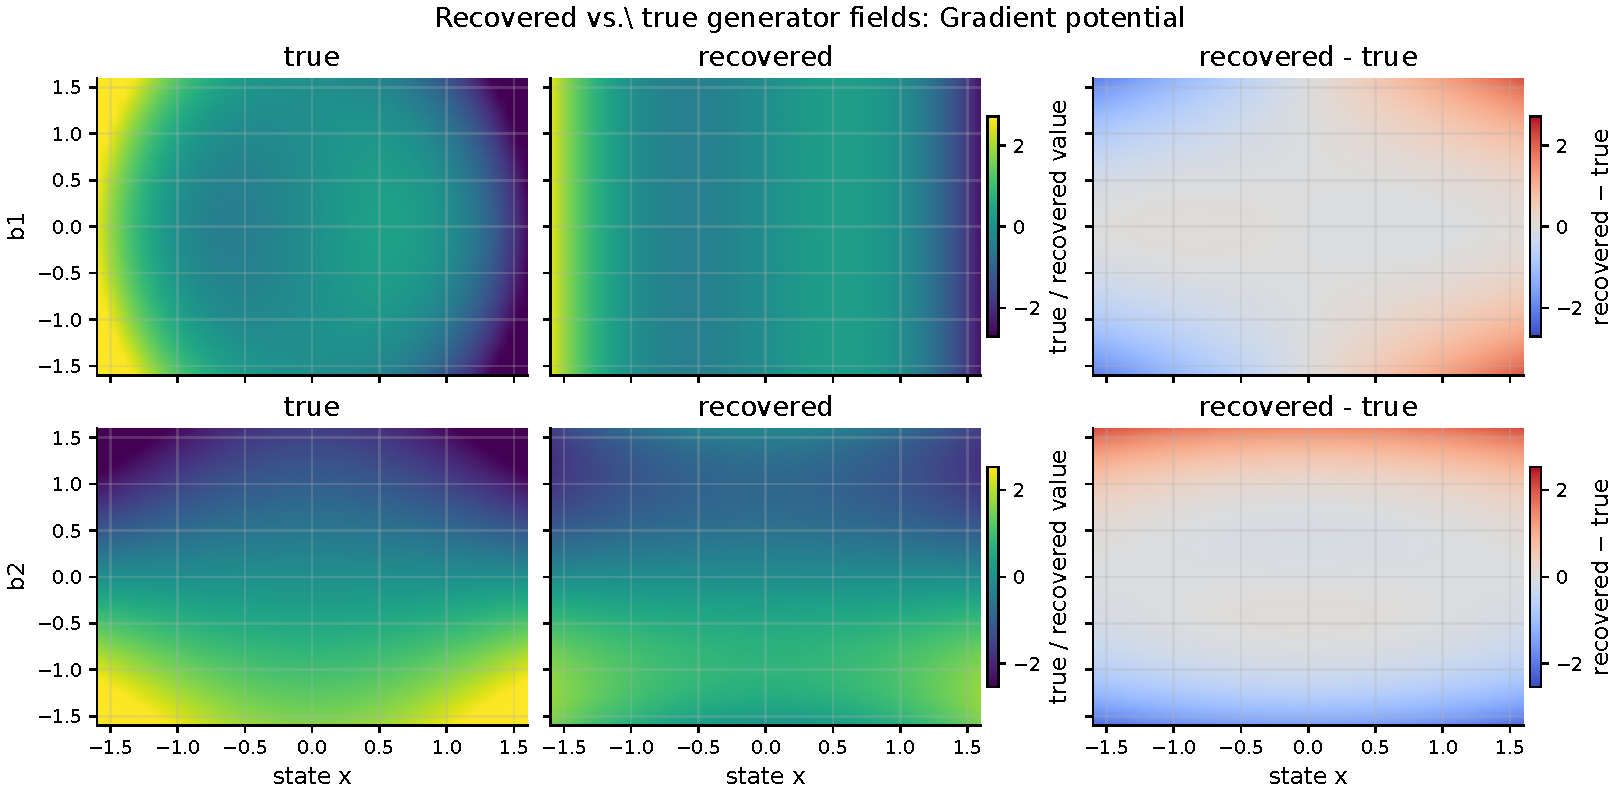
\includegraphics[width=0.86\linewidth]{datasheet_fields_gradient_potential.pdf}
\caption{Gradient potential: recovered vs.\ true generator fields (shared per-field colour scale; error column centred at zero).}\end{figure}
\paragraph{Verdict.} Drift $L^2(\mu)=0.246$, tensor rel-$L^2=0.024$, $a_{12}$ cosine $n/a$, PSD $1.00$, FP $0$ ($n$ seeds). \textbf{PASS}.
\medskip

\subsection{Maier--Stein}\label{sec:v62-maier-stein}
\paragraph{Context.} The Maier--Stein system is a standard benchmark in large-deviation and transition-path theory, modelling noise-activated escape over a non-gradient barrier. Its drift mixes a cubic bistability with a state-dependent transverse term $-(1+x^2)y$, whose $y$ and $x^2y$ pieces are strongly collinear on the sampled region; recovering the symbolic drift means the quasipotential and most-probable escape path become computable from data, which is why it is included despite being one of the harder fits.
\paragraph{System.} $$\drift=(X-X^3-\beta XY^2,\,-(1+X^2)Y),\ \beta=0.35,\ \diff=0.1225 I.$$
\paragraph{Generator.} Canonical non-gradient escape model. The $-(1+x^2)y$ term ($y$ and $x^2y$) is collinear on the sampled region; the small $-\beta xy^2$ term is the hardest to identify.
\paragraph{Recovery.} WG-SINDy recovers the drift at relative $L^2(\mu)=0.235$ and the diffusion tensor at $0.038$ relative error; the recovered drift reconstructs the potential landscape, its metastable wells, and the barrier between them. The active symbolic terms are recovered at selection rate one with no false positives; weaker secondary terms carry a lower selection rate.
\begin{figure}[H]\centering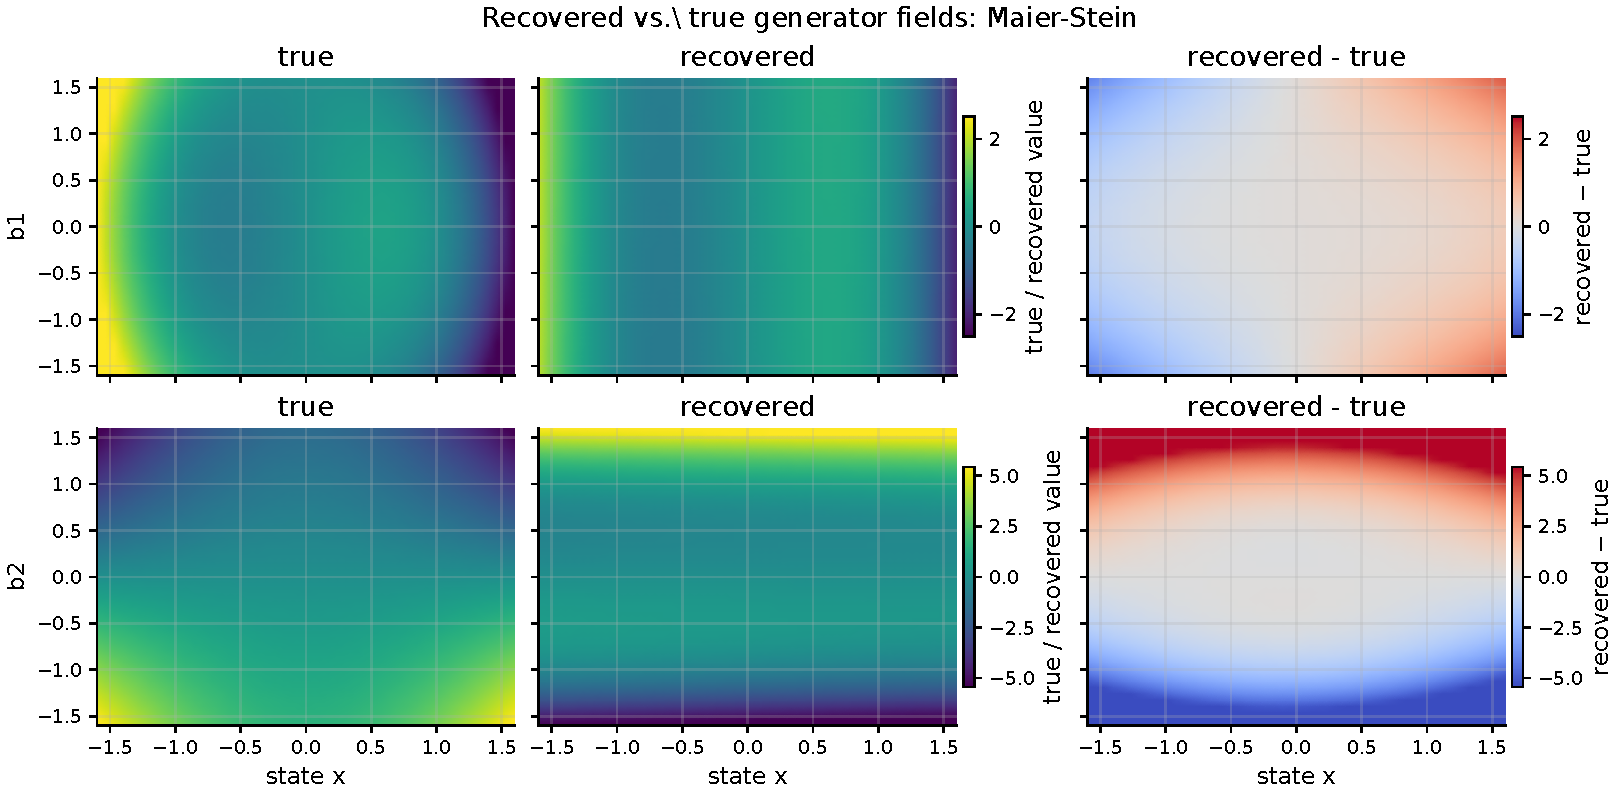
\includegraphics[width=0.86\linewidth]{datasheet_fields_maier_stein.pdf}
\caption{Maier--Stein: recovered vs.\ true generator fields (shared per-field colour scale; error column centred at zero).}\end{figure}
\paragraph{Verdict.} Drift $L^2(\mu)=0.235$, tensor rel-$L^2=0.038$, $a_{12}$ cosine $n/a$, PSD $1.00$, FP $0$ ($n$ seeds). \textbf{PASS}.
\medskip

\subsection{Duffing oscillator}\label{sec:v62-duffing}
\paragraph{Context.} The Duffing oscillator is a textbook nonlinear mechanical resonator written in position--velocity phase space. It tests recovery of a deterministic skeleton with a cubic restoring force and weak linear damping; because the damping coefficient is small relative to the restoring force and the noise, it is a controlled probe of how the estimator handles a genuine but low-amplitude term.
\paragraph{System.} $$\mathrm{d}X=Y\,\mathrm{d}t,\ \mathrm{d}Y=(-0.35Y+X-X^3)\mathrm{d}t+\sigma\mathrm{d}W,\ \diff_{22}=0.09.$$
\paragraph{Generator.} Noisy bistable oscillator in position--velocity form; the small damping $-0.35y$ is low-SNR and intermittently selected.
\paragraph{Recovery.} WG-SINDy recovers the drift at relative $L^2(\mu)=0.240$ and the diffusion tensor at $0.031$ relative error; the recovered drift reconstructs the potential landscape, its metastable wells, and the barrier between them. The active symbolic terms are recovered at selection rate one with no false positives; weaker secondary terms carry a lower selection rate.
\begin{figure}[H]\centering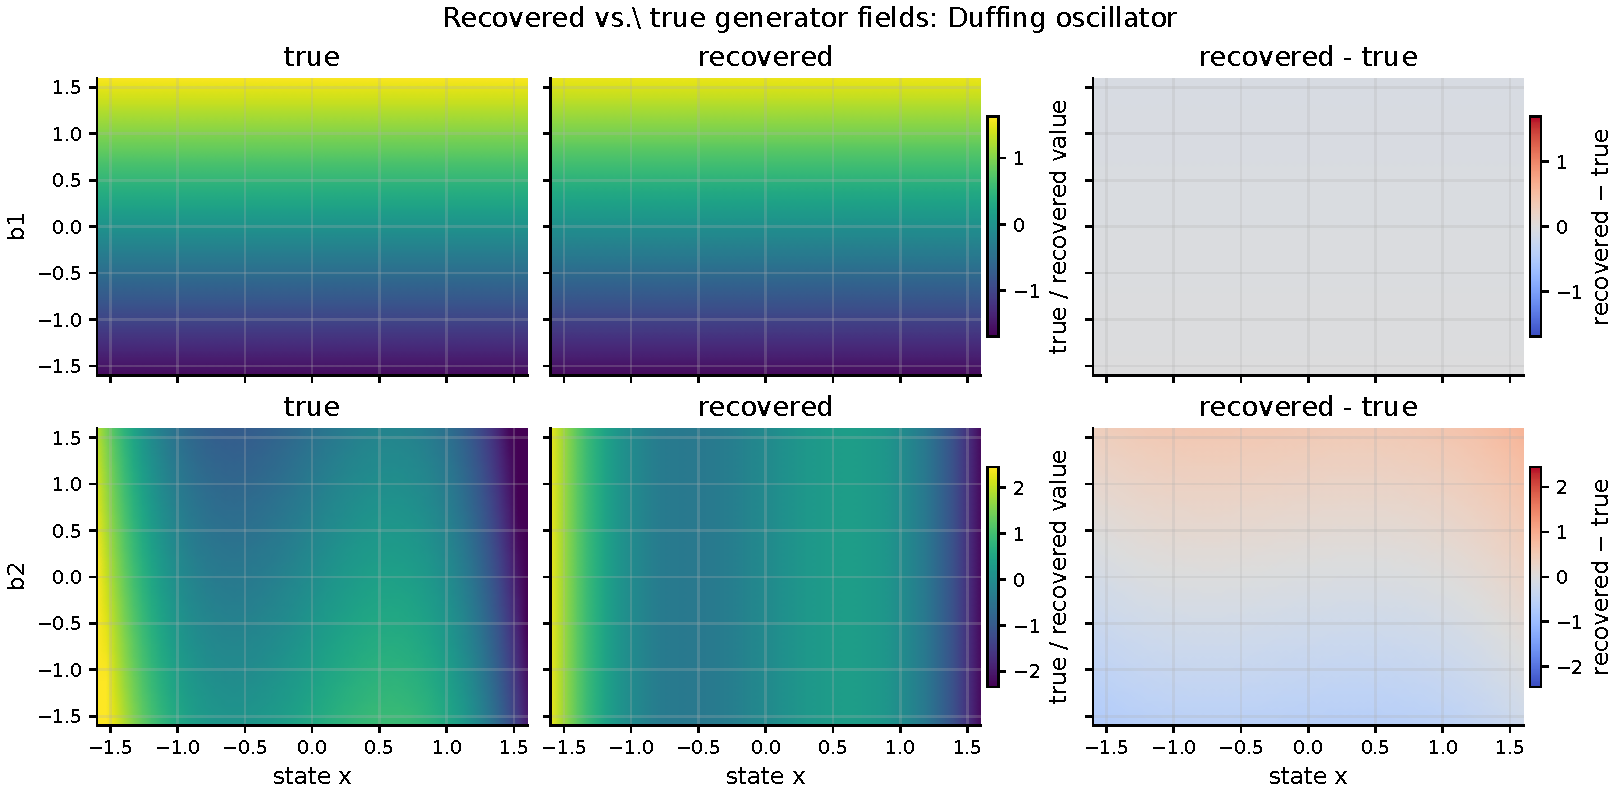
\includegraphics[width=0.86\linewidth]{datasheet_fields_duffing.pdf}
\caption{Duffing oscillator: recovered vs.\ true generator fields (shared per-field colour scale; error column centred at zero).}\end{figure}
\paragraph{Verdict.} Drift $L^2(\mu)=0.240$, tensor rel-$L^2=0.031$, $a_{12}$ cosine $n/a$, PSD $1.00$, FP $0$ ($n$ seeds). \textbf{PASS}.
\medskip

\subsection{Mueller--Brown}\label{sec:v62-mueller-brown}
\paragraph{Context.} The M\"uller--Brown surface is a standard multi-well molecular-dynamics benchmark. Its gradient drift is a sum of anisotropic Gaussians, strongly non-polynomial and stiff, and the small mobility depresses the drift signal; the diffusion is recovered while the drift is a representability null, an honest boundary that a radial-basis library, not a polynomial one, would be needed to cross.
\paragraph{System.} $$\drift=-m\nabla V_{\mathrm{MB}}\ (\text{four-Gaussian potential}),\ m=0.004.$$
\paragraph{Generator.} Stiff multi-well molecular potential; the strongly non-polynomial gradient is not spanned by a polynomial library. Named limit.
\paragraph{Recovery.} WG-SINDy recovers the drift at relative $L^2(\mu)=1.826$ and the diffusion tensor at $0.075$ relative error; the recovered drift reconstructs the potential landscape, its metastable wells, and the barrier between them. This is a named limit (registry declared failure or stress case): recovery fails for a physical or identifiability reason (library incompleteness, low signal-to-noise, degeneracy, or coverage), not an estimator defect.
\begin{figure}[H]\centering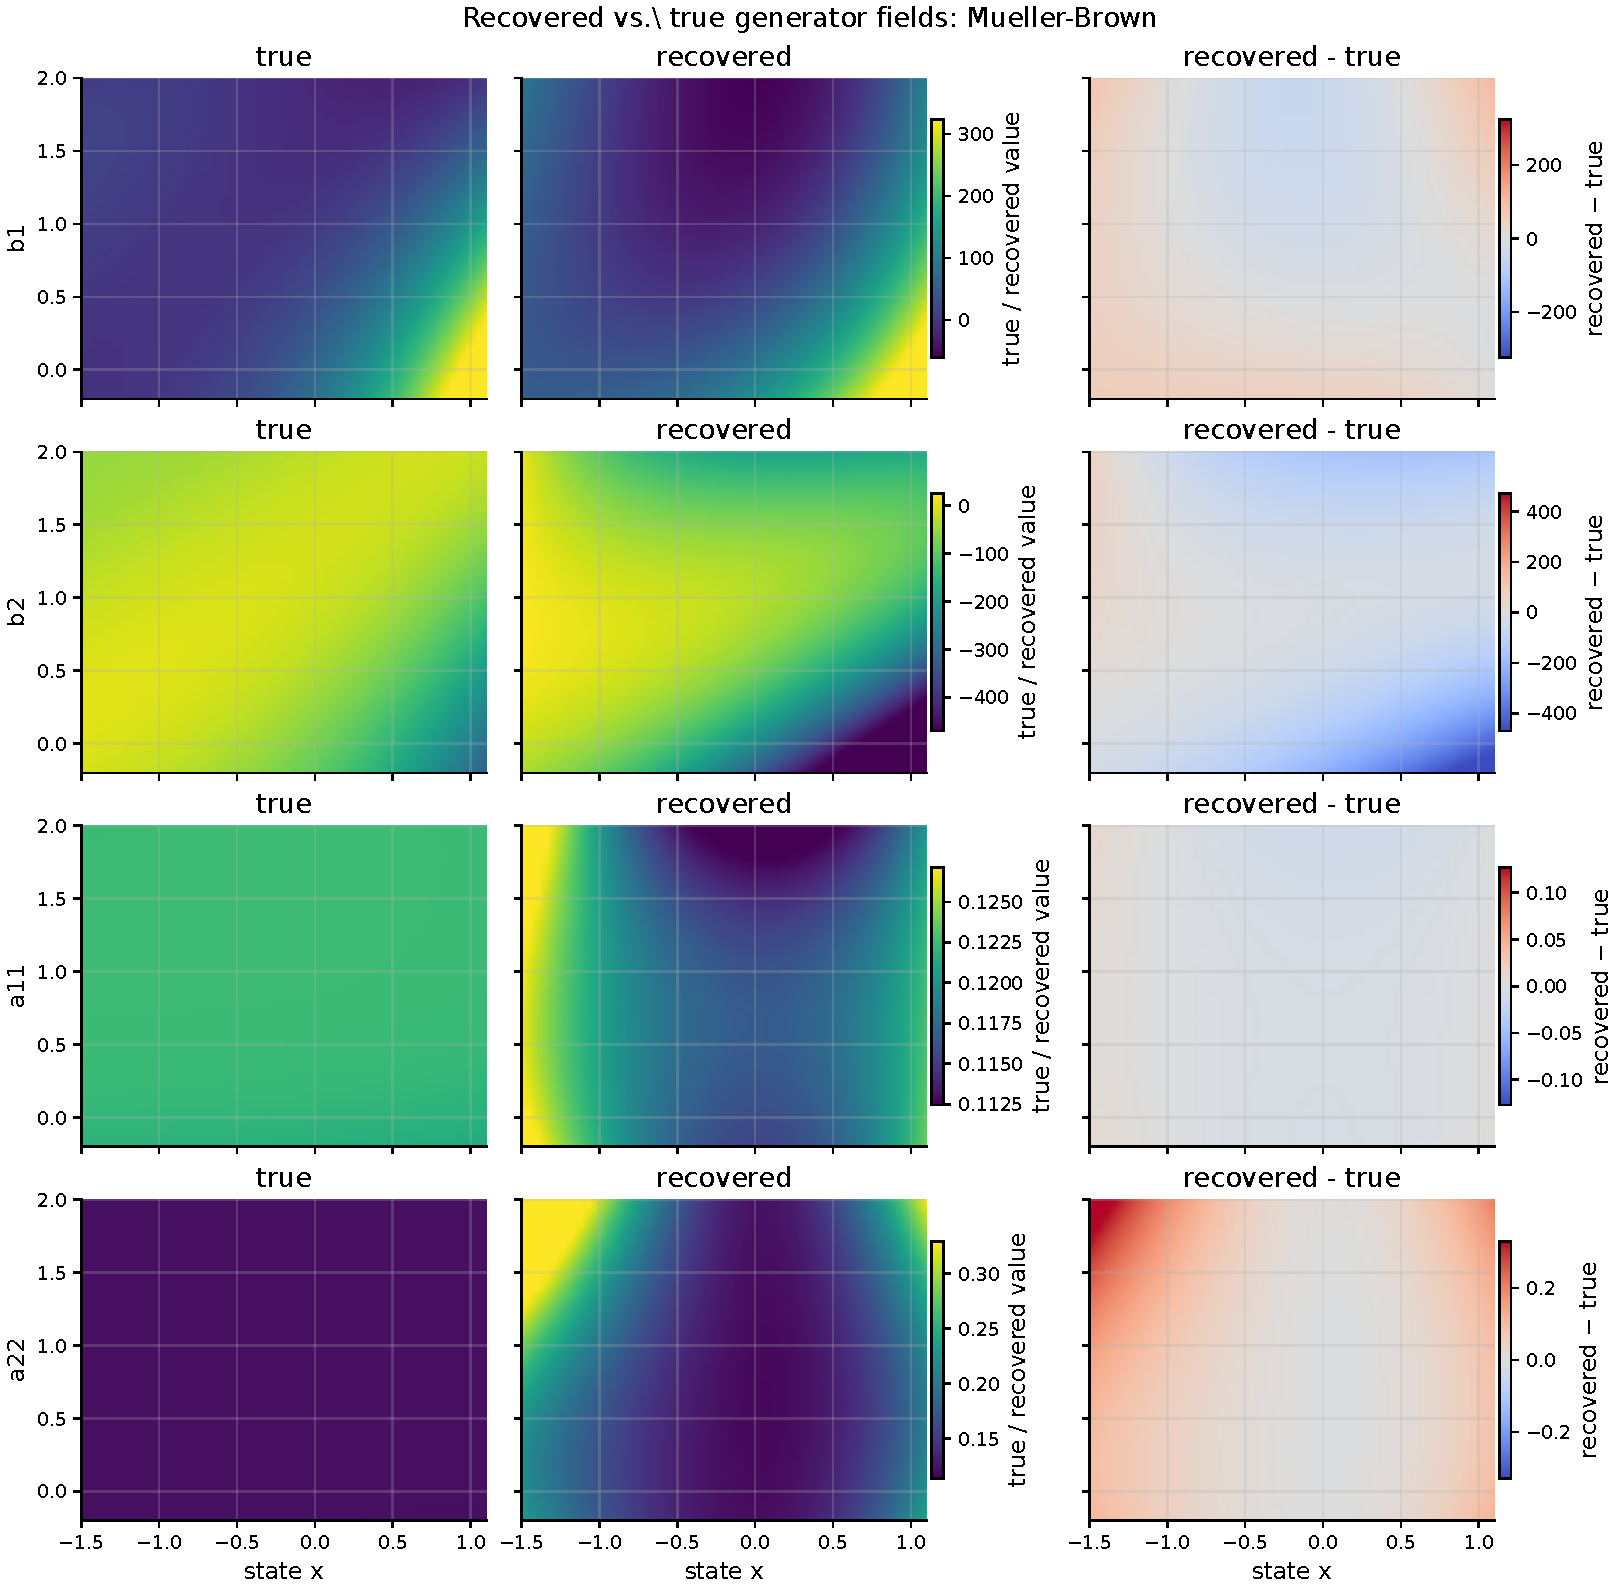
\includegraphics[width=0.86\linewidth]{datasheet_fields_mueller_brown.pdf}
\caption{Mueller--Brown: recovered vs.\ true generator fields (shared per-field colour scale; error column centred at zero).}\end{figure}
\paragraph{Verdict.} Drift $L^2(\mu)=1.826$, tensor rel-$L^2=0.075$, $a_{12}$ cosine $n/a$, PSD $1.00$, FP $0$ ($n$ seeds). \textbf{NAMED_NULL}.
\medskip
}{}
\IfFileExists{ds_multiplicative.tex}{% Auto-generated tight datasheets. Coefficients live in the aggregate R32 table. Source: results/v10/coeff_recovery_R32.csv
\paragraph{State-dependent (multiplicative) diffusion}\;

\subsection{Diagonal multiplicative}\label{sec:v62-diag-multiplicative}
\paragraph{Context.} A linear-drift system with \emph{state-dependent} (multiplicative) diffusion whose amplitude grows quadratically with position, the situation in population dynamics and fluctuating-environment models. It is the first test of recovering a diffusion \emph{field} rather than a constant, and of correctly returning a zero off-diagonal while both diagonal variances grow, i.e. not hallucinating leverage where none exists.
\paragraph{System.} $$\drift=-X,\ \diff=\mathrm{diag}(0.5+0.1x^2+0.1y^2,\,0.4+0.1x^2+0.1y^2).$$
\paragraph{Generator.} State-dependent diagonal diffusion (a field, not a constant); off-diagonal correctly zero. Quadratic diffusion terms are low-SNR.
\paragraph{Recovery.} WG-SINDy recovers the drift at relative $L^2(\mu)=0.200$ and the diffusion tensor at $0.112$ relative error; the recovered diffusion tensor is a position-dependent field giving the local fluctuation amplitude and relaxation. The active symbolic terms are recovered at selection rate one with no false positives; weaker secondary terms carry a lower selection rate.
% BEGIN METHOD COMPARISON TABLE
\paragraph{Matched method table.} Same-system comparison on the frozen matched ledger; lower is better except PSD.
\begin{center}\scriptsize
\begin{tabular}{lrrrr}
\toprule
Method & Drift & Tensor & $1-a_{12}$ cos. & PSD \\
\midrule
WG-SINDy & 0.201 & 0.111 & -- & 1.00 \\
Kramers-Moyal / stochastic SINDy & 0.524 & 0.076 & -- & 1.00 \\
Temporal Weak-SINDy & 1.00 & 0.137 & -- & 1.00 \\
gEDMD & 0.525 & 0.080 & -- & 1.00 \\
Vanilla SINDy (FD-STLSQ) & 1.53 & 0.172 & -- & 1.00 \\
\bottomrule
\end{tabular}
\end{center}
% END METHOD COMPARISON TABLE

\begin{figure}[H]\centering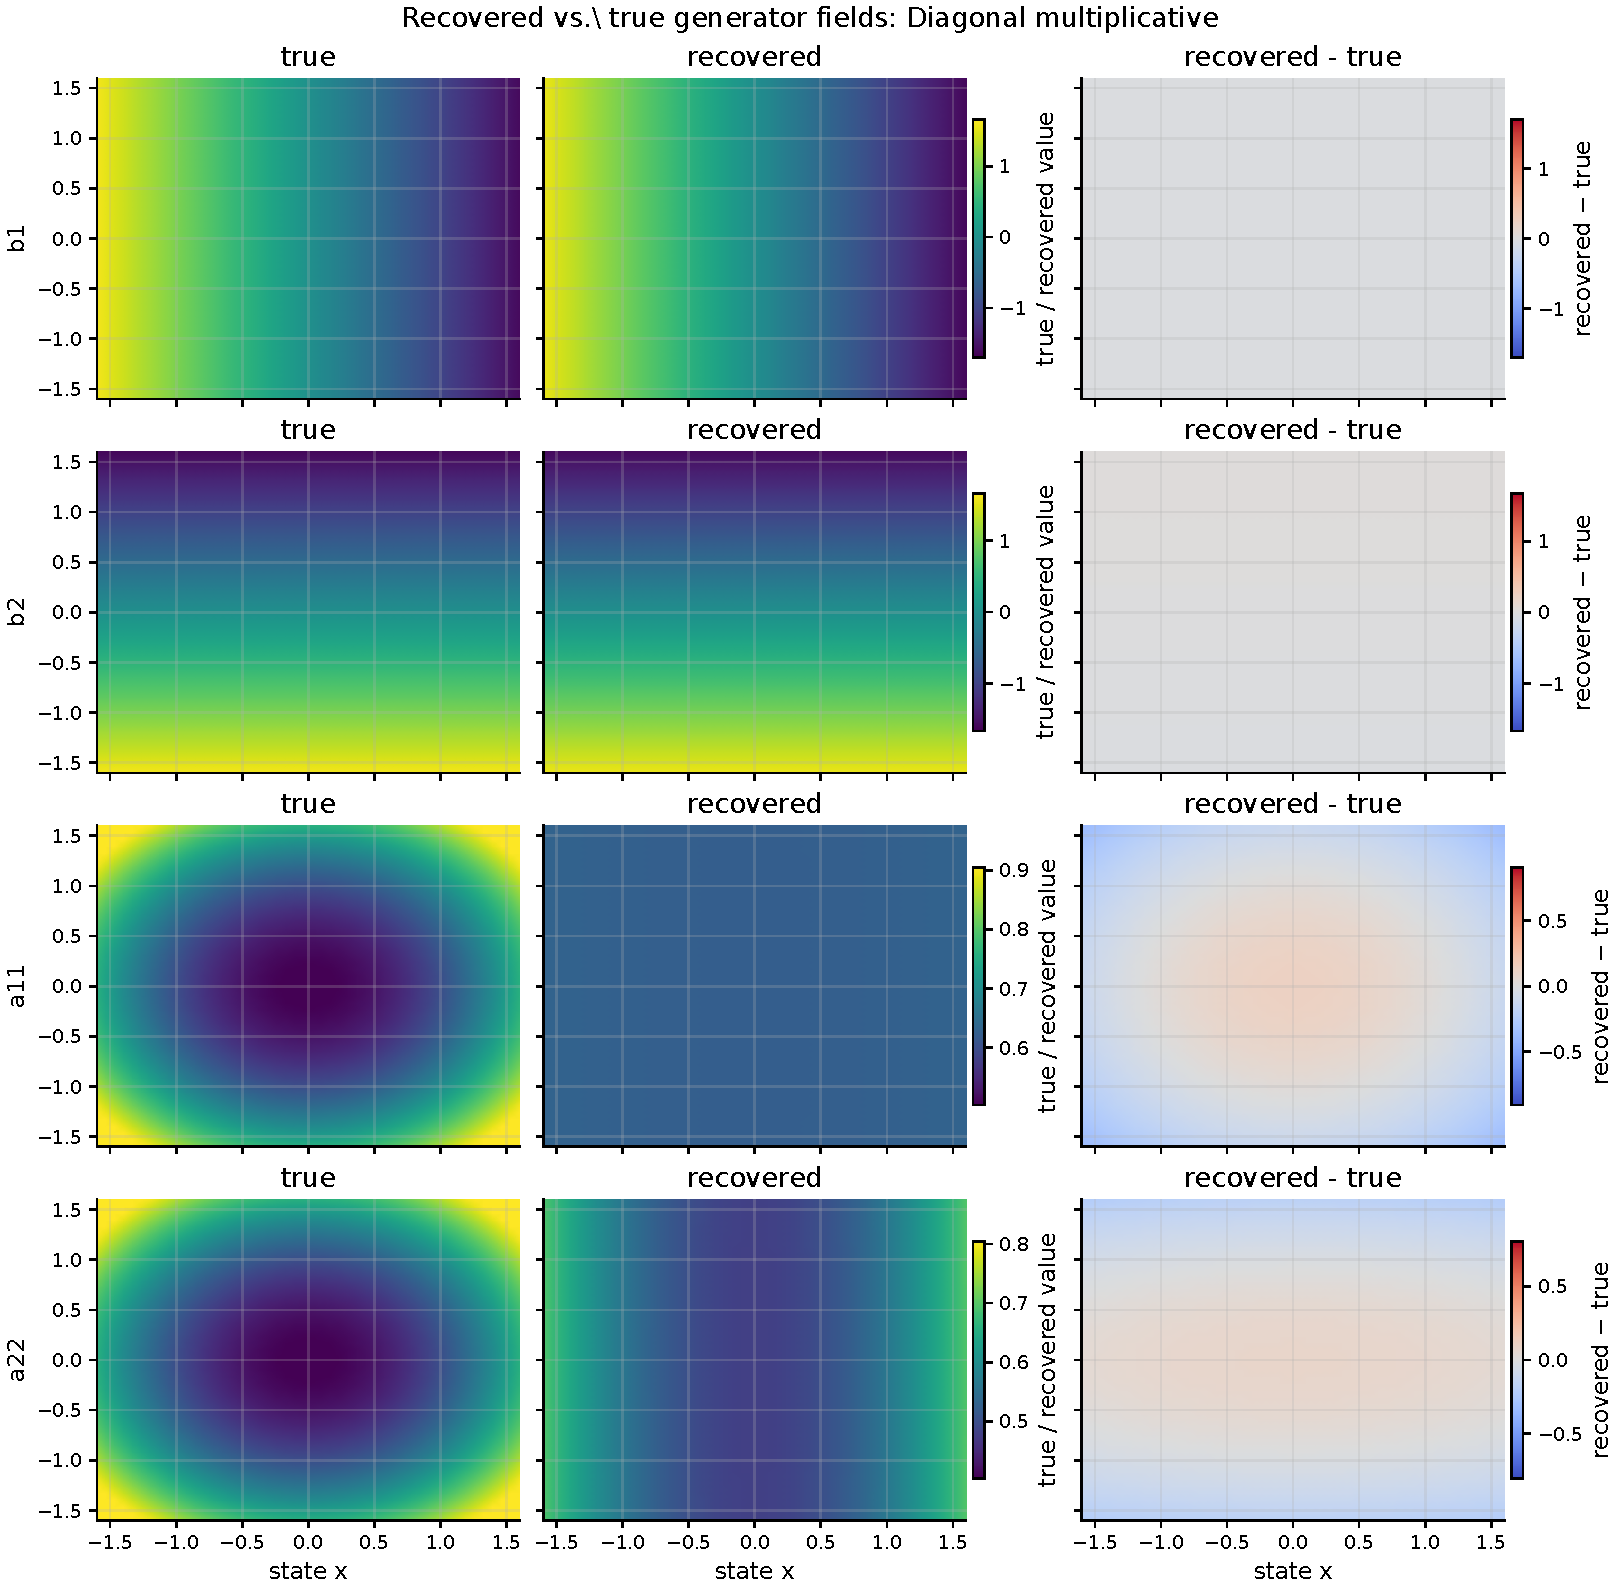
\includegraphics[width=0.86\linewidth]{datasheet_fields_diag_multiplicative.pdf}
\caption{Diagonal multiplicative: recovered vs.\ true generator fields (shared per-field colour scale; error column centred at zero).}\end{figure}
\paragraph{Verdict.} Drift $L^2(\mu)=0.200$, tensor rel-$L^2=0.112$, $a_{12}$ cosine $n/a$, PSD $1.00$, FP $0$ ($n$ seeds). \textbf{PASS}.
\medskip

\subsection{Non-diagonal Cholesky}\label{sec:v62-nondiag-cholesky}
\paragraph{Context.} The hardest clean synthetic test of a fully \emph{state-dependent off-diagonal} diffusion, constructed through a Cholesky factor so the target is positive semidefinite everywhere by design. The off-diagonal varies in space and changes sign across the axes, so it probes both the recovery of a spatially varying leverage field and the structural PSD guarantee that a naive entrywise regression of cross-increments would violate.
\paragraph{System.} $$\diff=LL^\top,\ L=\begin{psmallmatrix}0.5+0.1x^2&0\\0.2xy&0.4+0.1y^2\end{psmallmatrix},\ \drift=-X.$$
\paragraph{Generator.} State-dependent off-diagonal diffusion, PSD by construction; the leading $a_{12}\!\approx\!0.1xy$ term is recovered, higher-order factor terms are weak.
\paragraph{Recovery.} WG-SINDy recovers the drift at relative $L^2(\mu)=0.204$ and the diffusion tensor at $0.079$ relative error, with off-diagonal (leverage) cosine $0.988$; the recovered diffusion tensor is a position-dependent field giving the local fluctuation amplitude and relaxation. The active symbolic terms are recovered at selection rate one with no false positives; weaker secondary terms carry a lower selection rate.
% BEGIN METHOD COMPARISON TABLE
\paragraph{Matched method table.} Same-system comparison on the frozen matched ledger; lower is better except PSD.
\begin{center}\scriptsize
\begin{tabular}{lrrrr}
\toprule
Method & Drift & Tensor & $1-a_{12}$ cos. & PSD \\
\midrule
WG-SINDy & 0.208 & 0.079 & 0.012 & 1.00 \\
Kramers-Moyal / stochastic SINDy & 1.09 & 0.157 & 0.356 & 1.00 \\
Temporal Weak-SINDy & 1.00 & 0.125 & 0.238 & 1.00 \\
gEDMD & 0.452 & 0.065 & 0.094 & 1.00 \\
Vanilla SINDy (FD-STLSQ) & 3.66 & 0.594 & 0.860 & 0.908 \\
\bottomrule
\end{tabular}
\end{center}
% END METHOD COMPARISON TABLE

\begin{figure}[H]\centering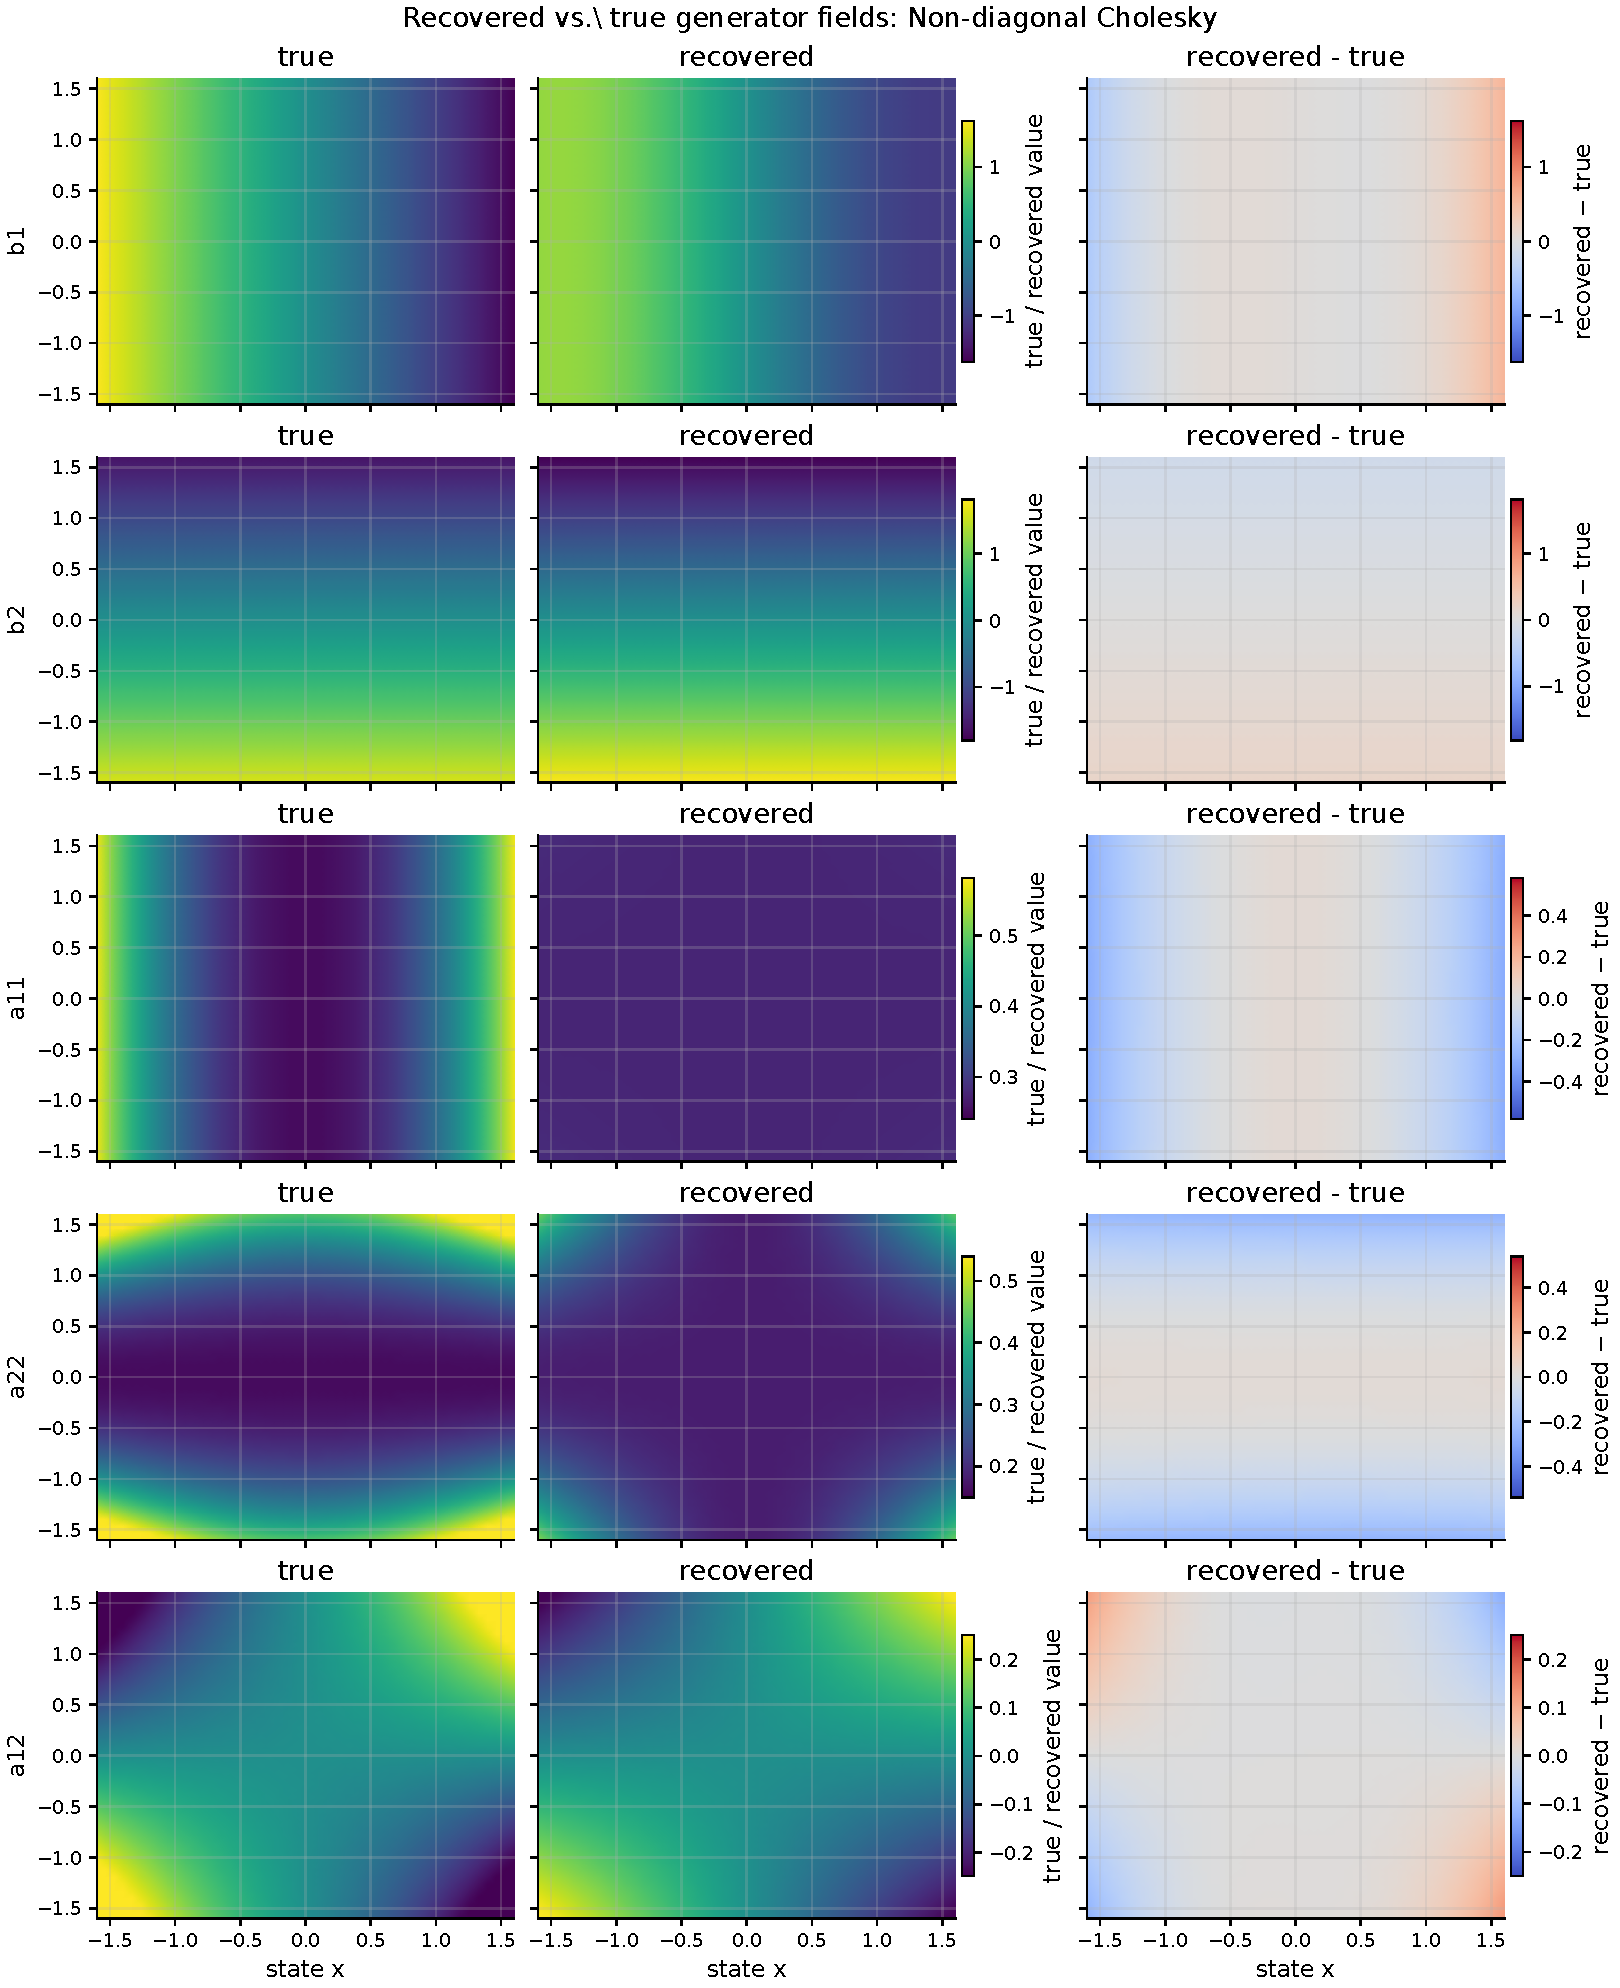
\includegraphics[width=0.86\linewidth]{datasheet_fields_nondiag_cholesky.pdf}
\caption{Non-diagonal Cholesky: recovered vs.\ true generator fields (shared per-field colour scale; error column centred at zero).}\end{figure}
\paragraph{Verdict.} Drift $L^2(\mu)=0.204$, tensor rel-$L^2=0.079$, $a_{12}$ cosine $0.988$, PSD $1.00$, FP $0$ ($n$ seeds). \textbf{PASS}.
\medskip
}{}
\IfFileExists{ds_financial.tex}{% Auto-generated tight datasheets. Coefficients live in the aggregate R32 table. Source: results/v10/coeff_recovery_R32.csv
\paragraph{Financial / stochastic-volatility systems}\;

\subsection{Log-Heston}\label{sec:v62-heston-logsv}
\paragraph{Context.} The Heston model is a cornerstone of mathematical finance, with stochastic instantaneous variance driving the asset. In the numerically stable log-price coordinate it is the flagship leverage system: the negative price--variance correlation $\rho$ enters only through the off-diagonal $\diff_{12}=\rho\xi v$, the single parameter that shapes the implied-volatility skew used in option pricing. It also exposes the central honest limit, the risk-neutral log-price drift $\mu-\tfrac12 v$, whose per-step signal is some four orders of magnitude below the diffusion noise.
\paragraph{System.} $$\mathrm{d}X=(\mu-\tfrac12 v)\mathrm{d}t+\sqrt{v}\mathrm{d}W_1,\ \mathrm{d}v=\kappa(\theta-v)\mathrm{d}t+\xi\sqrt{v}\mathrm{d}W_2.$$
\paragraph{Generator.} Flagship leverage system. $\drift_v=\kappa(\theta-v)$ variance mean reversion; $\diff_{11}=v$, $\diff_{22}=\xi^2 v$, $\diff_{12}=\rho\xi v$ leverage. Log-price drift $\mu-\tfrac12 v$ is the low-SNR null.
\paragraph{Recovery.} WG-SINDy recovers the drift at relative $L^2(\mu)=0.143$ and the diffusion tensor at $0.054$ relative error, with off-diagonal (leverage) cosine $0.999$; the off-diagonal yields the price--variance leverage correlation alongside the variance mean-reversion and vol-of-vol. The active symbolic terms are recovered at selection rate one with no false positives; weaker secondary terms carry a lower selection rate.
% BEGIN METHOD COMPARISON TABLE
\paragraph{Matched method table.} Same-system comparison on the frozen matched ledger; lower is better except PSD.
\begin{center}\scriptsize
\begin{tabular}{lrrrr}
\toprule
Method & Drift & Tensor & $1-a_{12}$ cos. & PSD \\
\midrule
WG-SINDy & 0.143 & 0.054 & 1.3e-03 & 1.00 \\
Kramers-Moyal / stochastic SINDy & 0.486 & 0.038 & 1.5e-03 & 0.994 \\
Temporal Weak-SINDy & 1.00 & 0.080 & 1.8e-03 & 1.00 \\
gEDMD & 0.545 & 0.074 & 4.7e-03 & 0.926 \\
Vanilla SINDy (FD-STLSQ) & 1.62 & 0.113 & 0.019 & 0.944 \\
\bottomrule
\end{tabular}
\end{center}
% END METHOD COMPARISON TABLE

\begin{figure}[H]\centering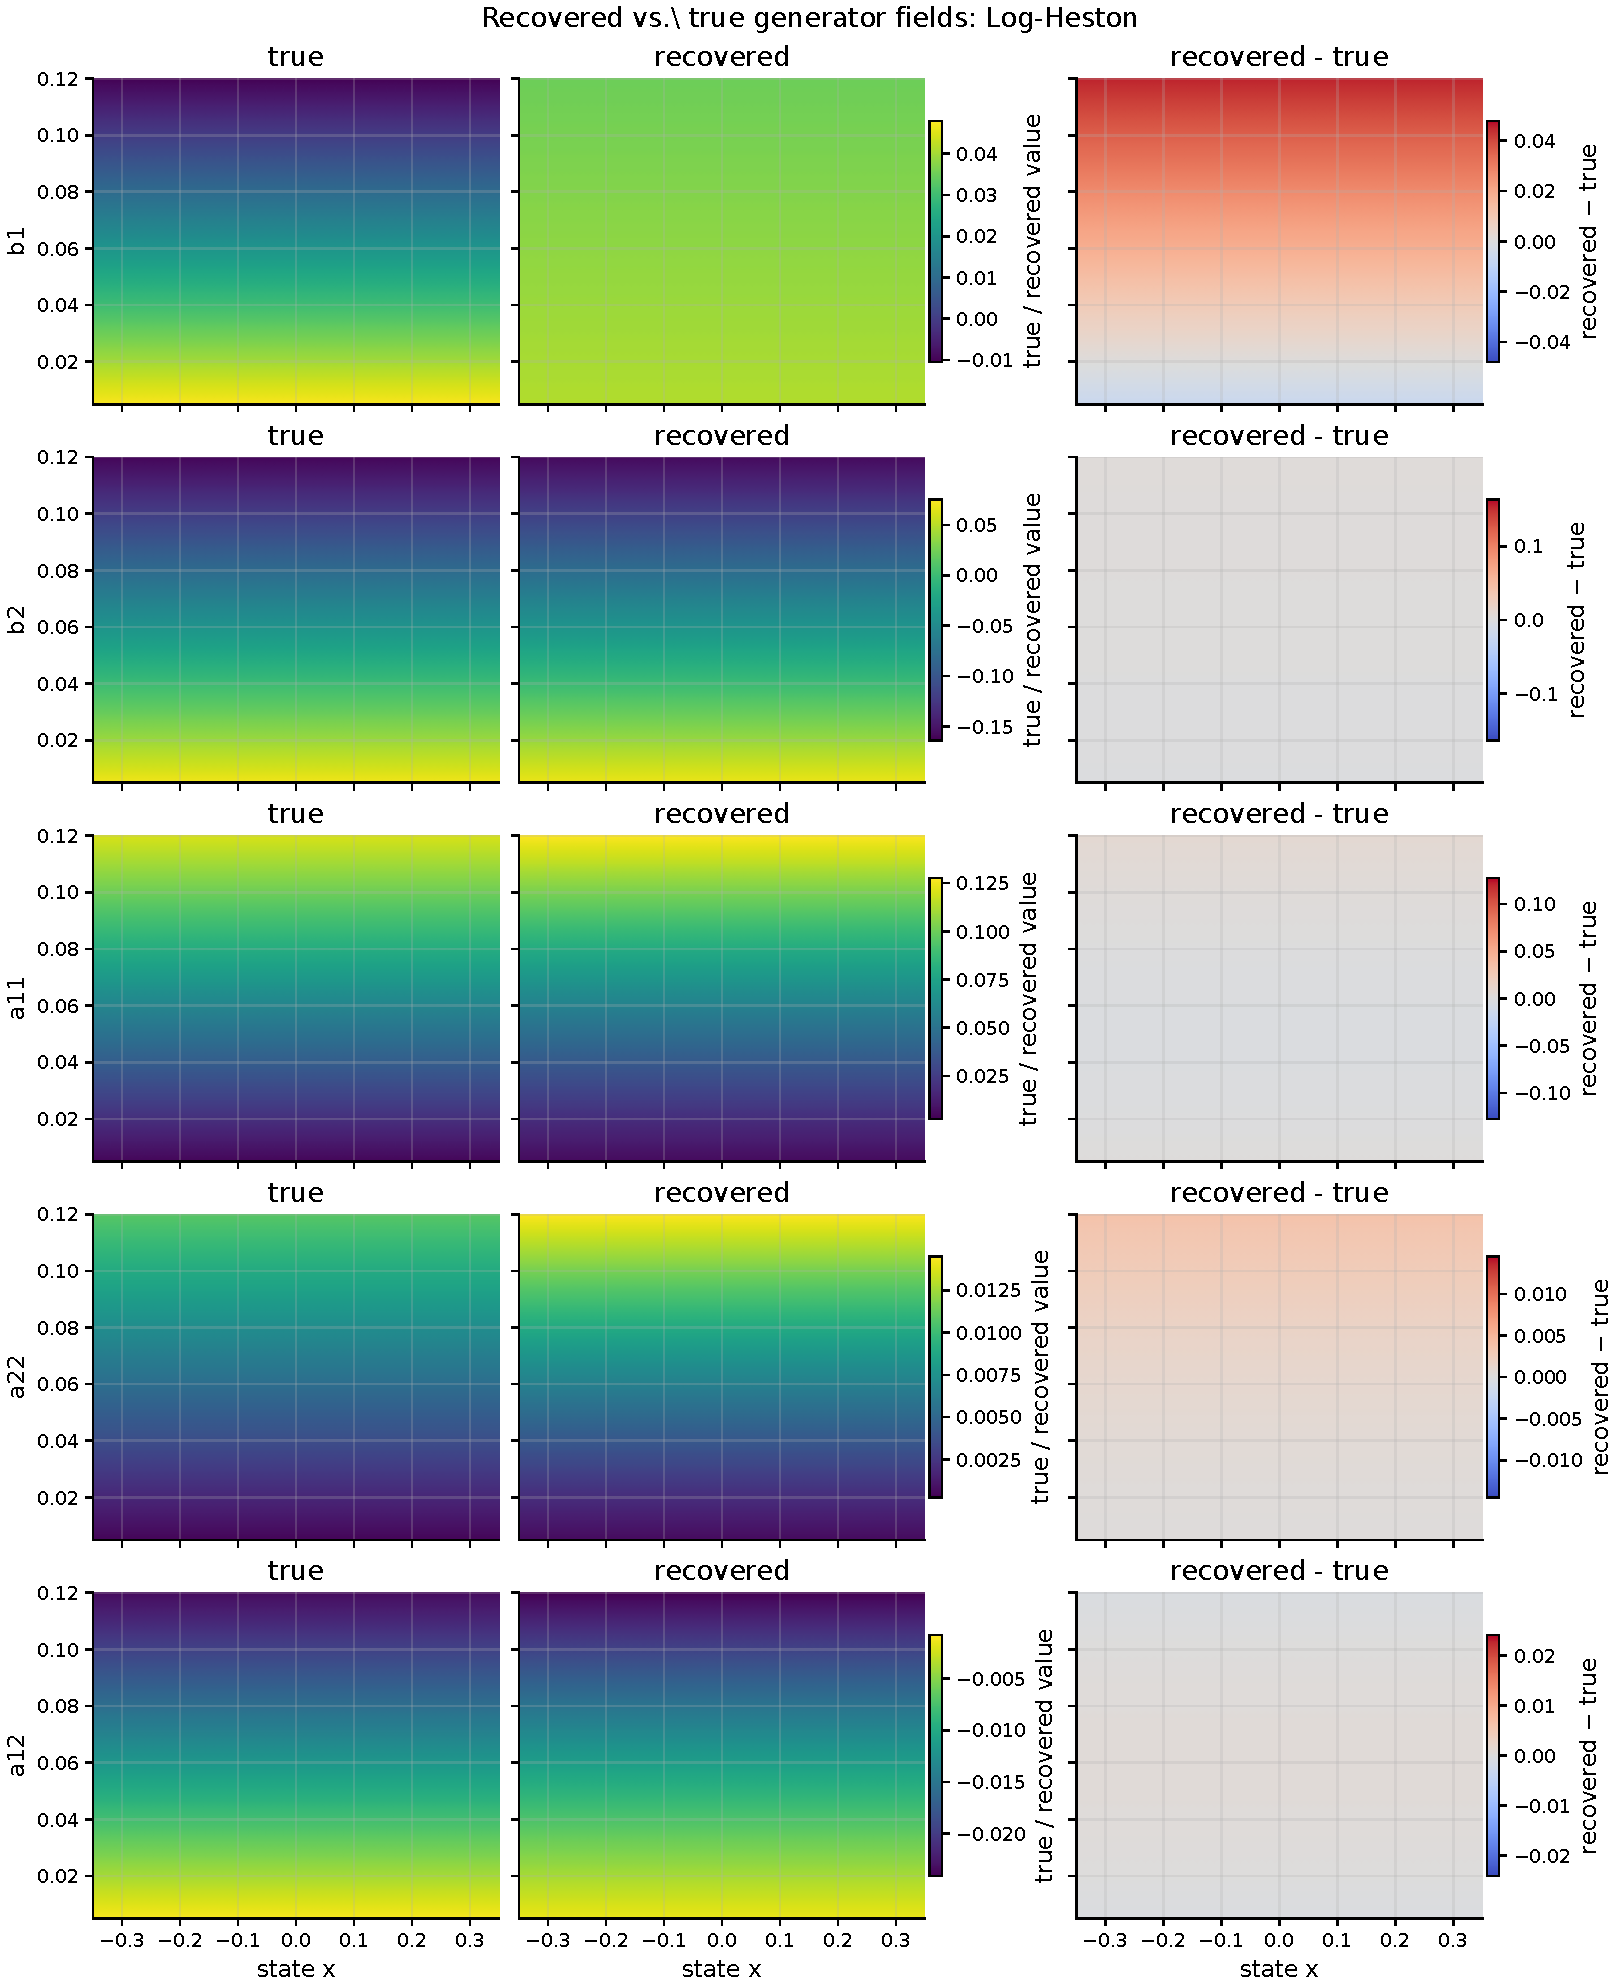
\includegraphics[width=0.86\linewidth]{datasheet_fields_heston_logsv.pdf}
\caption{Log-Heston: recovered vs.\ true generator fields (shared per-field colour scale; error column centred at zero).}\end{figure}
\paragraph{Verdict.} Drift $L^2(\mu)=0.143$, tensor rel-$L^2=0.054$, $a_{12}$ cosine $0.999$, PSD $1.00$, FP $0$ ($n$ seeds). \textbf{PASS}.
\medskip

\subsection{Heston $(S,V)$}\label{sec:v62-heston-sv}
\paragraph{Context.} The raw-price formulation of the same Heston dynamics, retained to show the leverage result is not an artefact of the log transform. Its diagonal variance $S^2v$ spans an enormous dynamic range, the very ill-conditioning that motivates practitioners to take logs; recovering the leverage and variance generator here demonstrates that the anisotropic kernels and whitening absorb extreme coordinate scaling without manual transformation.
\paragraph{System.} $$\mathrm{d}S=\mu S\,\mathrm{d}t+S\sqrt{v}\mathrm{d}W_1,\ \mathrm{d}v=\kappa(\theta-v)\mathrm{d}t+\xi\sqrt{v}\mathrm{d}W_2.$$
\paragraph{Generator.} Raw-price Heston: $\diff_{11}=S^2v$ (large dynamic range), $\diff_{12}=\rho\xi Sv$ leverage. Recovered despite the scale; price drift $\mu S$ is the low-SNR null.
\paragraph{Recovery.} WG-SINDy recovers the drift at relative $L^2(\mu)=0.273$ and the diffusion tensor at $0.089$ relative error, with off-diagonal (leverage) cosine $0.993$; the off-diagonal yields the price--variance leverage correlation alongside the variance mean-reversion and vol-of-vol. The active symbolic terms are recovered at selection rate one with no false positives; weaker secondary terms carry a lower selection rate.
% BEGIN METHOD COMPARISON TABLE
\paragraph{Matched method table.} Same-system comparison on the frozen matched ledger; lower is better except PSD.
\begin{center}\scriptsize
\begin{tabular}{lrrrr}
\toprule
Method & Drift & Tensor & $1-a_{12}$ cos. & PSD \\
\midrule
WG-SINDy & 0.276 & 0.089 & 7.3e-03 & 1.00 \\
Kramers-Moyal / stochastic SINDy & 0.727 & 0.115 & 4.9e-03 & 0.973 \\
Temporal Weak-SINDy & 1.12 & 0.152 & 4.6e-03 & 0.938 \\
gEDMD & 1.15 & 0.151 & 9.3e-03 & 0.923 \\
Vanilla SINDy (FD-STLSQ) & 2.56 & 0.273 & 0.037 & 0.920 \\
\bottomrule
\end{tabular}
\end{center}
% END METHOD COMPARISON TABLE

\begin{figure}[H]\centering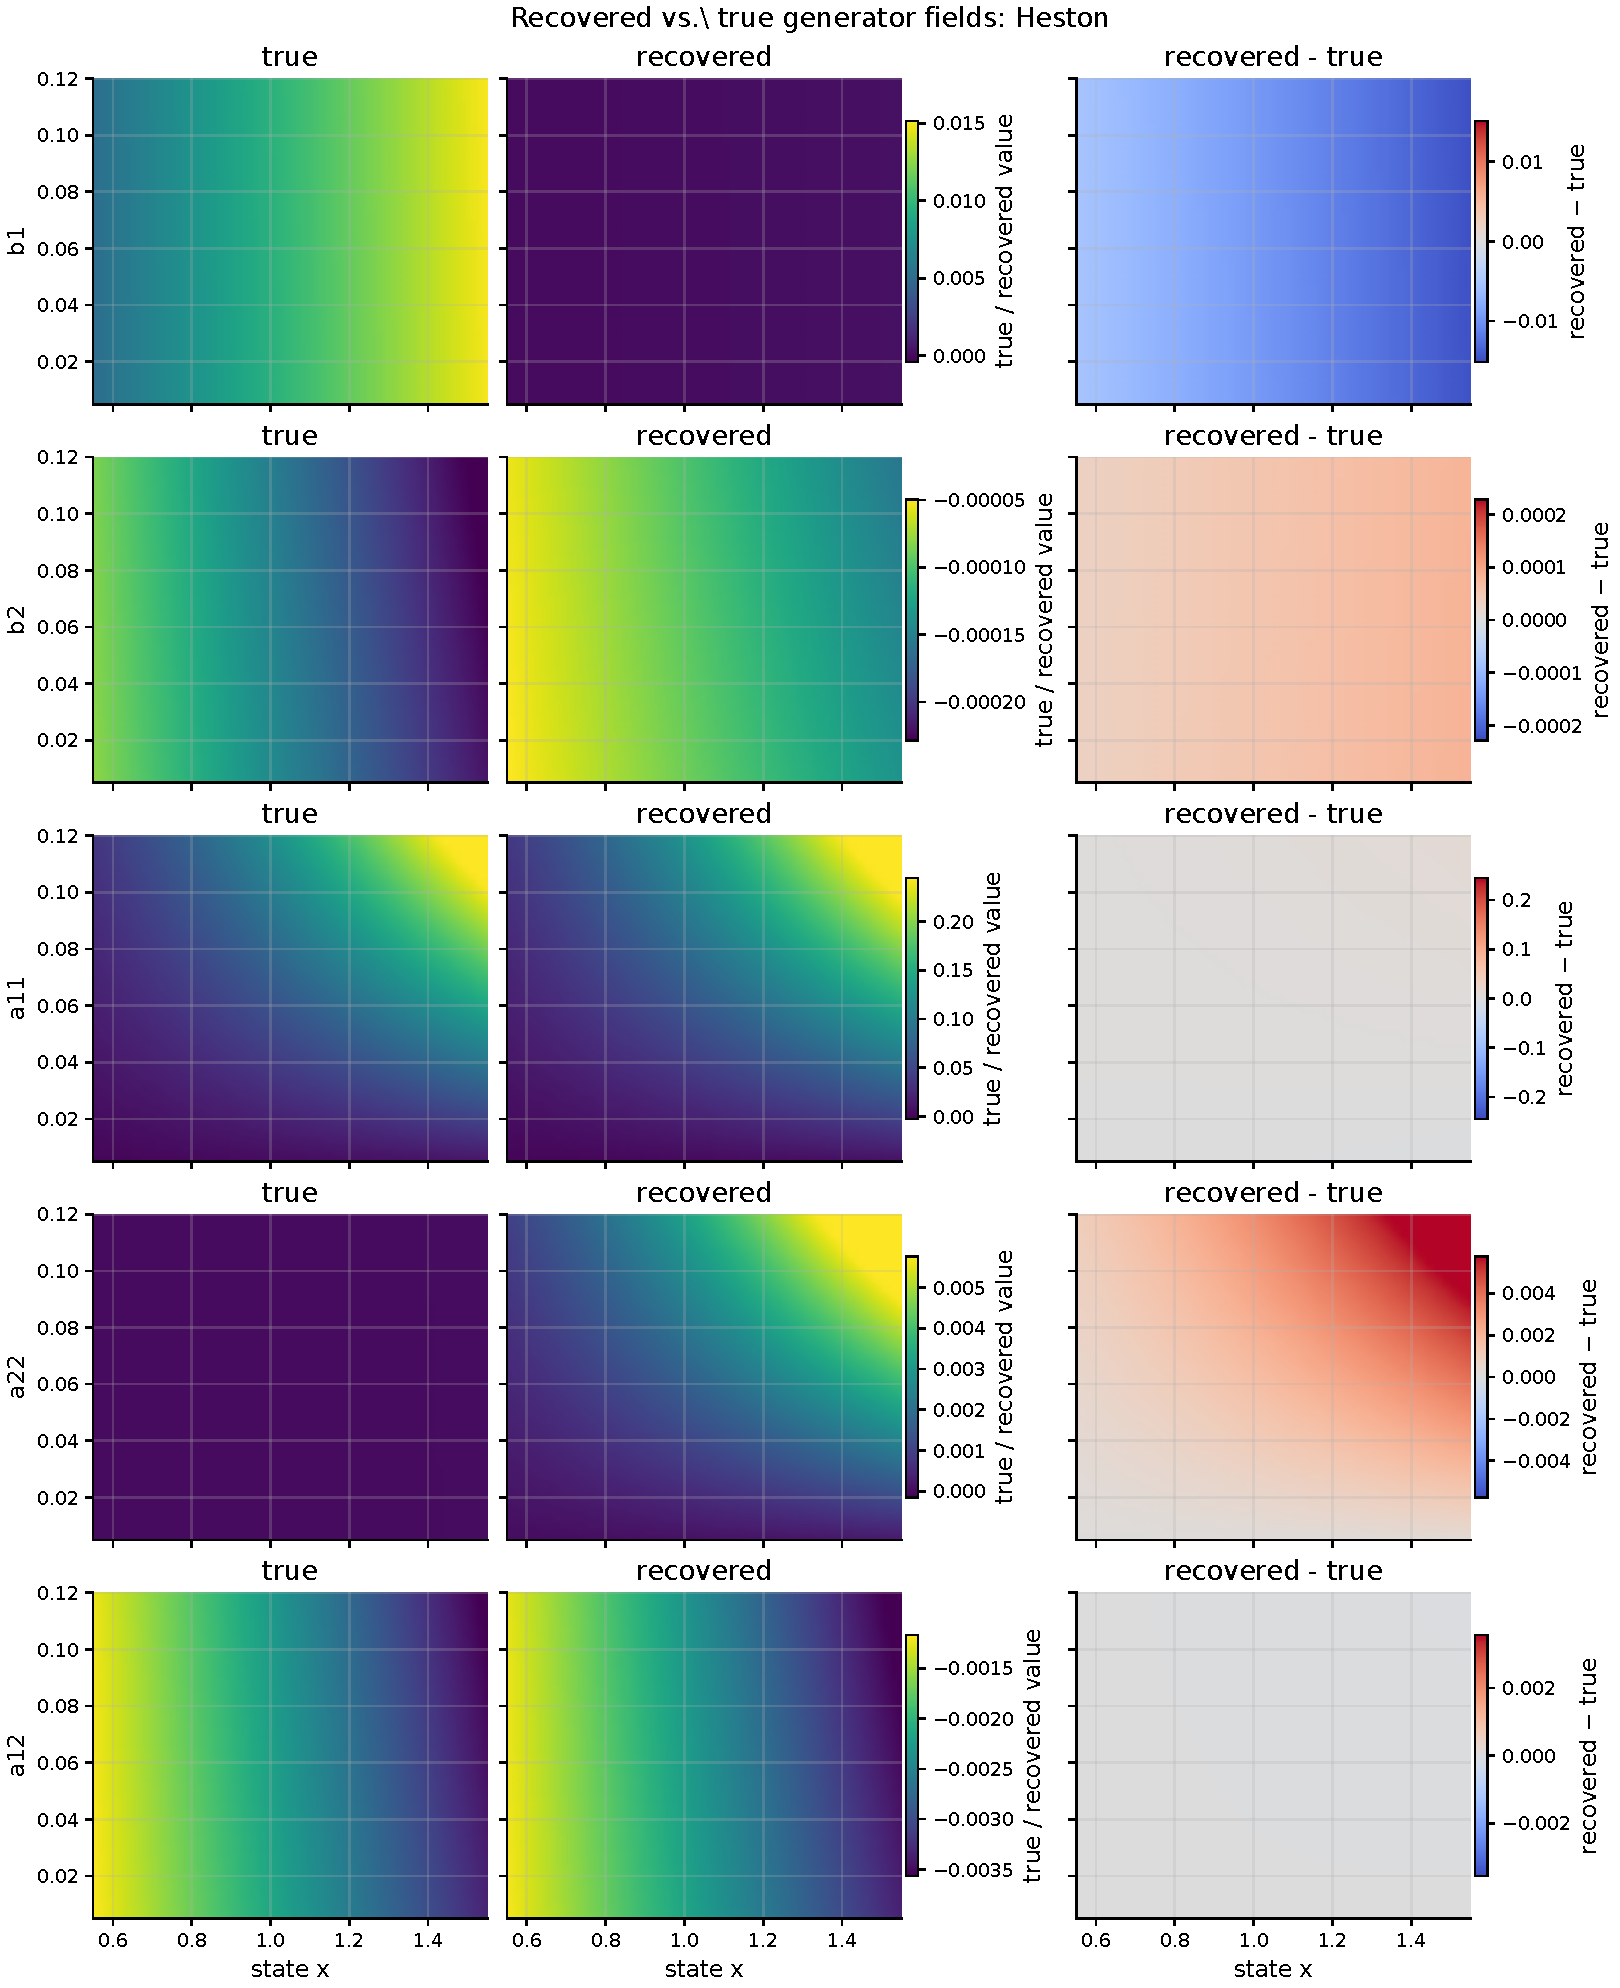
\includegraphics[width=0.86\linewidth]{datasheet_fields_heston_sv.pdf}
\caption{Heston $(S,V)$: recovered vs.\ true generator fields (shared per-field colour scale; error column centred at zero).}\end{figure}
\paragraph{Verdict.} Drift $L^2(\mu)=0.273$, tensor rel-$L^2=0.089$, $a_{12}$ cosine $0.993$, PSD $1.00$, FP $0$ ($n$ seeds). \textbf{PASS}.
\medskip

\subsection{CIR pair}\label{sec:v62-cir-pair}
\paragraph{Context.} A pair of correlated Cox--Ingersoll--Ross processes, the building block of multi-factor interest-rate and competing-population models. Its off-diagonal diffusion is genuinely non-polynomial ($\propto\sqrt{xy}$), so it tests whether the estimator accommodates a square-root feature library; both square-root mean-reverting drifts are recovered, unlike the stochastic-volatility log-price drift, because mean reversion carries adequate signal.
\paragraph{System.} $$\mathrm{d}X=\kappa(\theta-X)\mathrm{d}t+\xi\sqrt{X}\mathrm{d}W_1,\ \mathrm{d}Y=\kappa(\theta-Y)\mathrm{d}t+\xi\sqrt{Y}\mathrm{d}W_2.$$
\paragraph{Generator.} Correlated square-root processes; $\diff_{12}=\rho\xi^2\sqrt{xy}$ needs the square-root library F. Both mean-reverting drifts recover.
\paragraph{Recovery.} WG-SINDy recovers the drift at relative $L^2(\mu)=0.393$ and the diffusion tensor at $0.116$ relative error, with off-diagonal (leverage) cosine $0.995$; the off-diagonal yields the price--variance leverage correlation alongside the variance mean-reversion and vol-of-vol. The active symbolic terms are recovered at selection rate one with no false positives; weaker secondary terms carry a lower selection rate.
% BEGIN METHOD COMPARISON TABLE
\paragraph{Matched method table.} Same-system comparison on the frozen matched ledger; lower is better except PSD.
\begin{center}\scriptsize
\begin{tabular}{lrrrr}
\toprule
Method & Drift & Tensor & $1-a_{12}$ cos. & PSD \\
\midrule
WG-SINDy & 0.392 & 0.117 & 4.8e-03 & 1.00 \\
Kramers-Moyal / stochastic SINDy & 1.64 & 0.213 & 4.7e-03 & 0.938 \\
Temporal Weak-SINDy & 1.03 & 0.203 & 5.7e-03 & 0.970 \\
gEDMD & 8.36 & 1.29 & 0.211 & 0.784 \\
Vanilla SINDy (FD-STLSQ) & 8.21 & 0.741 & 0.078 & 0.731 \\
\bottomrule
\end{tabular}
\end{center}
% END METHOD COMPARISON TABLE

\begin{figure}[H]\centering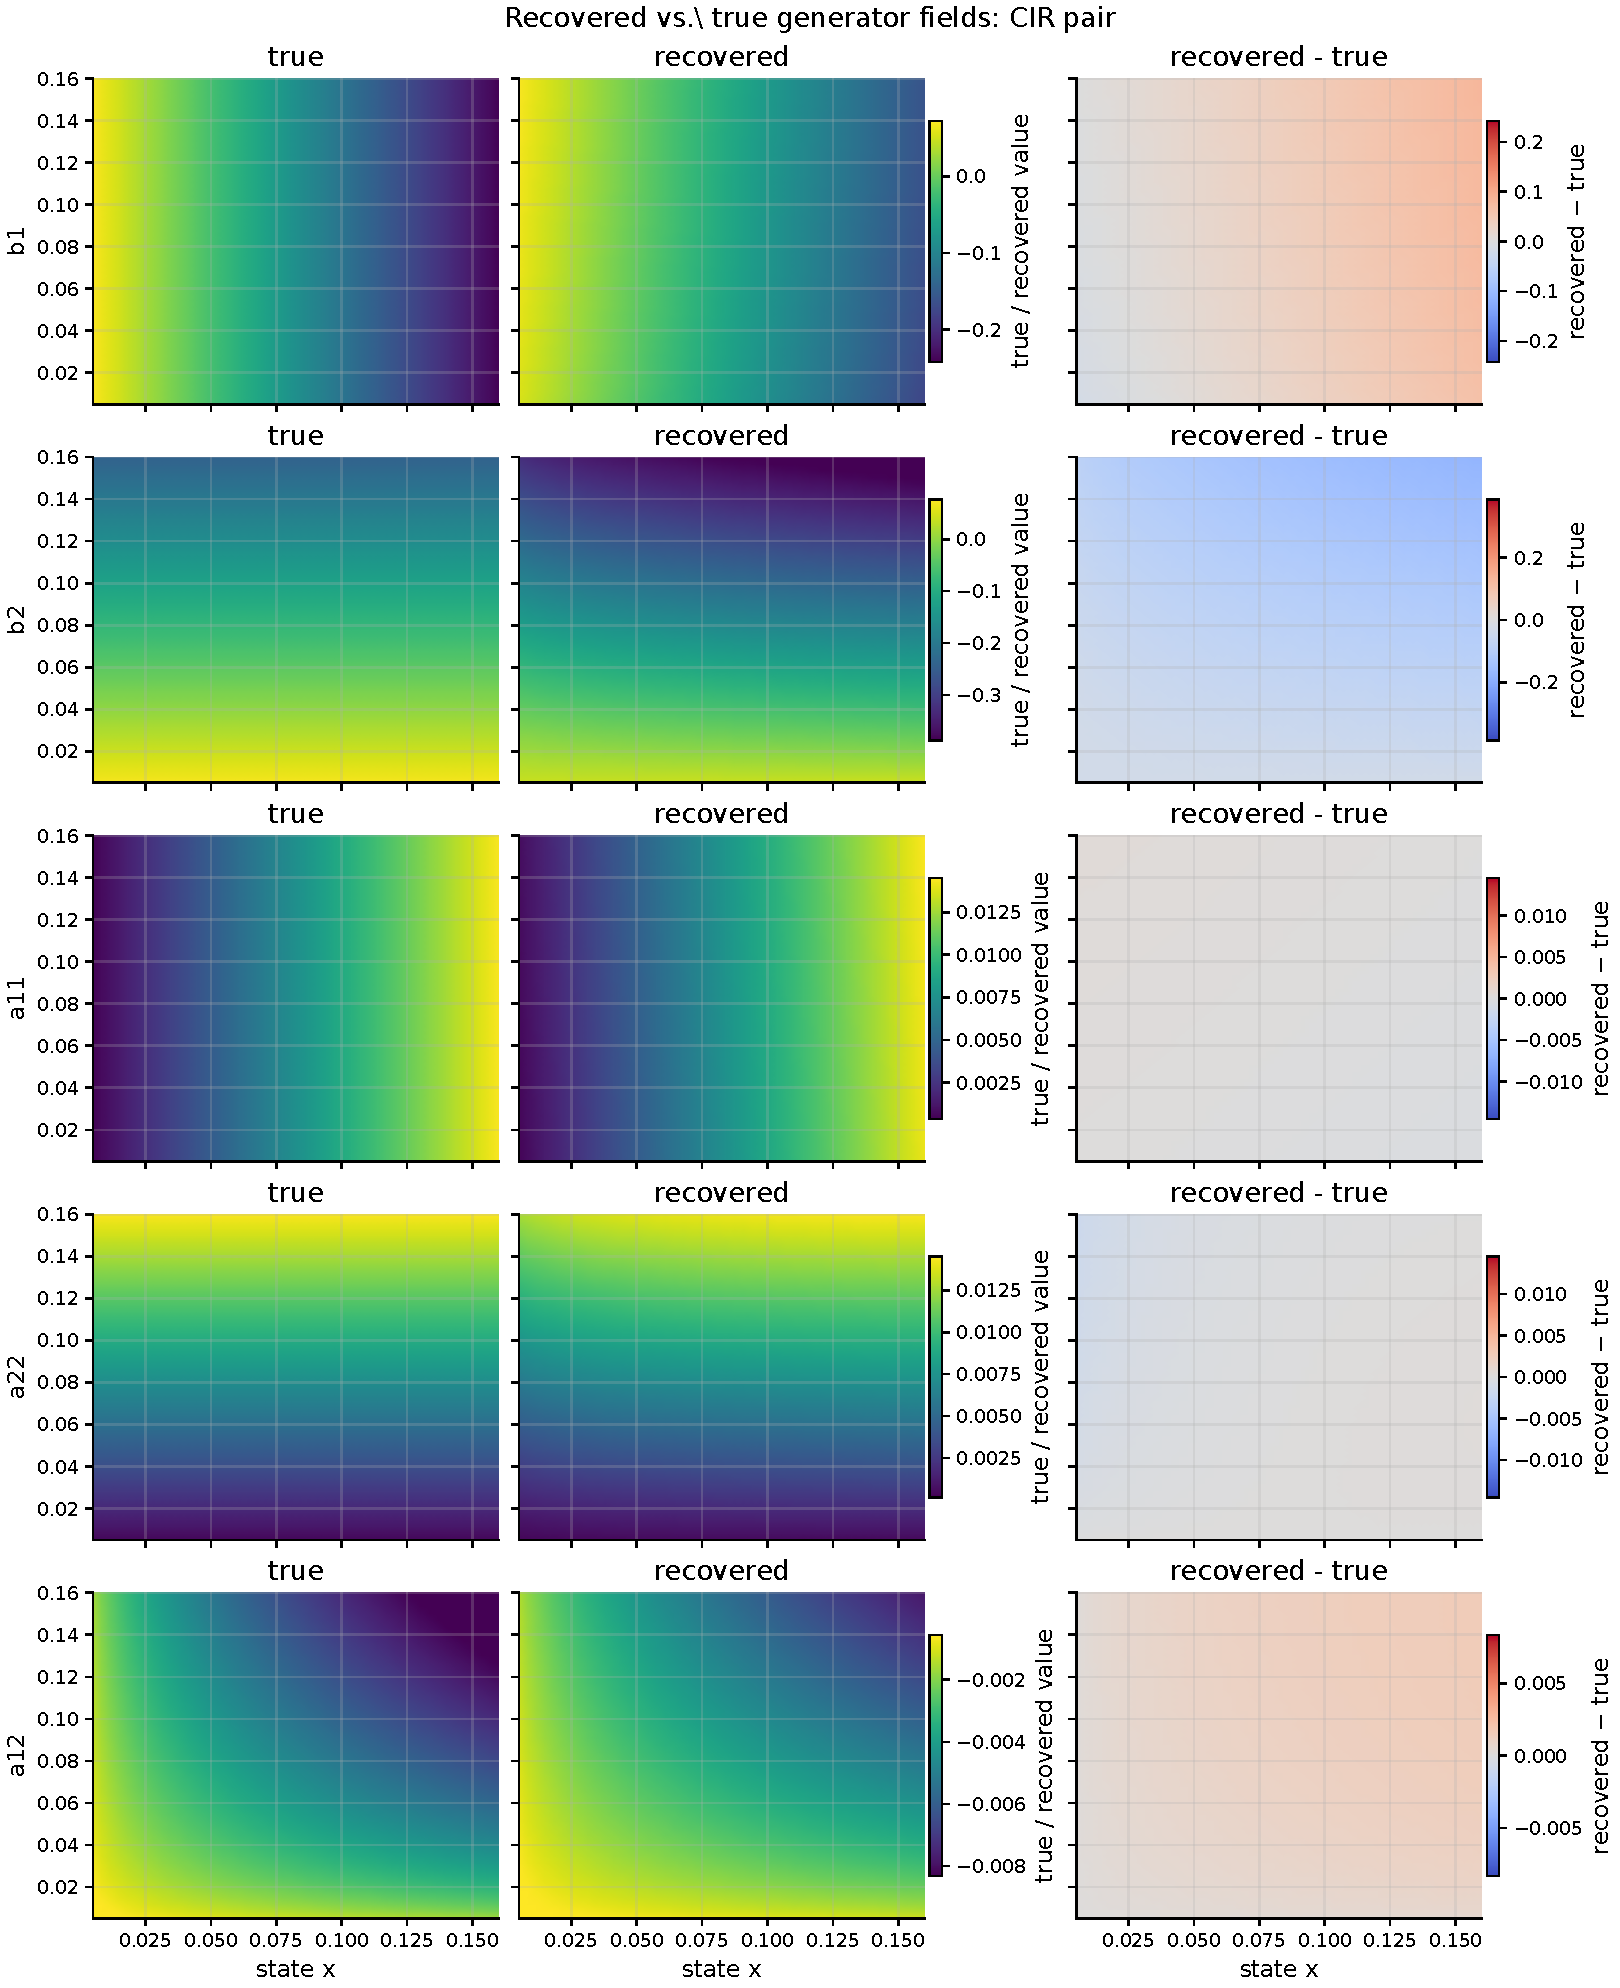
\includegraphics[width=0.86\linewidth]{datasheet_fields_cir_pair.pdf}
\caption{CIR pair: recovered vs.\ true generator fields (shared per-field colour scale; error column centred at zero).}\end{figure}
\paragraph{Verdict.} Drift $L^2(\mu)=0.393$, tensor rel-$L^2=0.116$, $a_{12}$ cosine $0.995$, PSD $1.00$, FP $0$ ($n$ seeds). \textbf{PASS}.
\medskip

\subsection{SABR}\label{sec:v62-sabr}
\paragraph{Context.} The SABR model is an industry-standard stochastic-volatility specification for interest-rate and FX smiles. It is a driftless martingale with power-law ($F^\beta$) diffusion, so it tests two edges at once: a generator with no drift to recover (which must come back as exactly zero) and a fractional-power diffusion that a polynomial library can only approximate, making it a named limit on the tensor while the leverage sign is still recovered.
\paragraph{System.} $$\mathrm{d}F=\sigma F^\beta\mathrm{d}W_1,\ \mathrm{d}\sigma=\nu\sigma\mathrm{d}W_2,\ \beta=0.5.$$
\paragraph{Generator.} Driftless martingale with power-law diffusion; leverage cosine recovers, the $F^{2\beta}$ power-law is only approximately spanned. Named limit.
\paragraph{Recovery.} WG-SINDy recovers the drift at relative $L^2(\mu)=--$ and the diffusion tensor at $0.195$ relative error, with off-diagonal (leverage) cosine $0.990$; the off-diagonal yields the price--variance leverage correlation alongside the variance mean-reversion and vol-of-vol. This is a named limit (fragile physics or identifiability limit): recovery fails for a physical or identifiability reason (library incompleteness, low signal-to-noise, degeneracy, or coverage), not an estimator defect.
\begin{figure}[H]\centering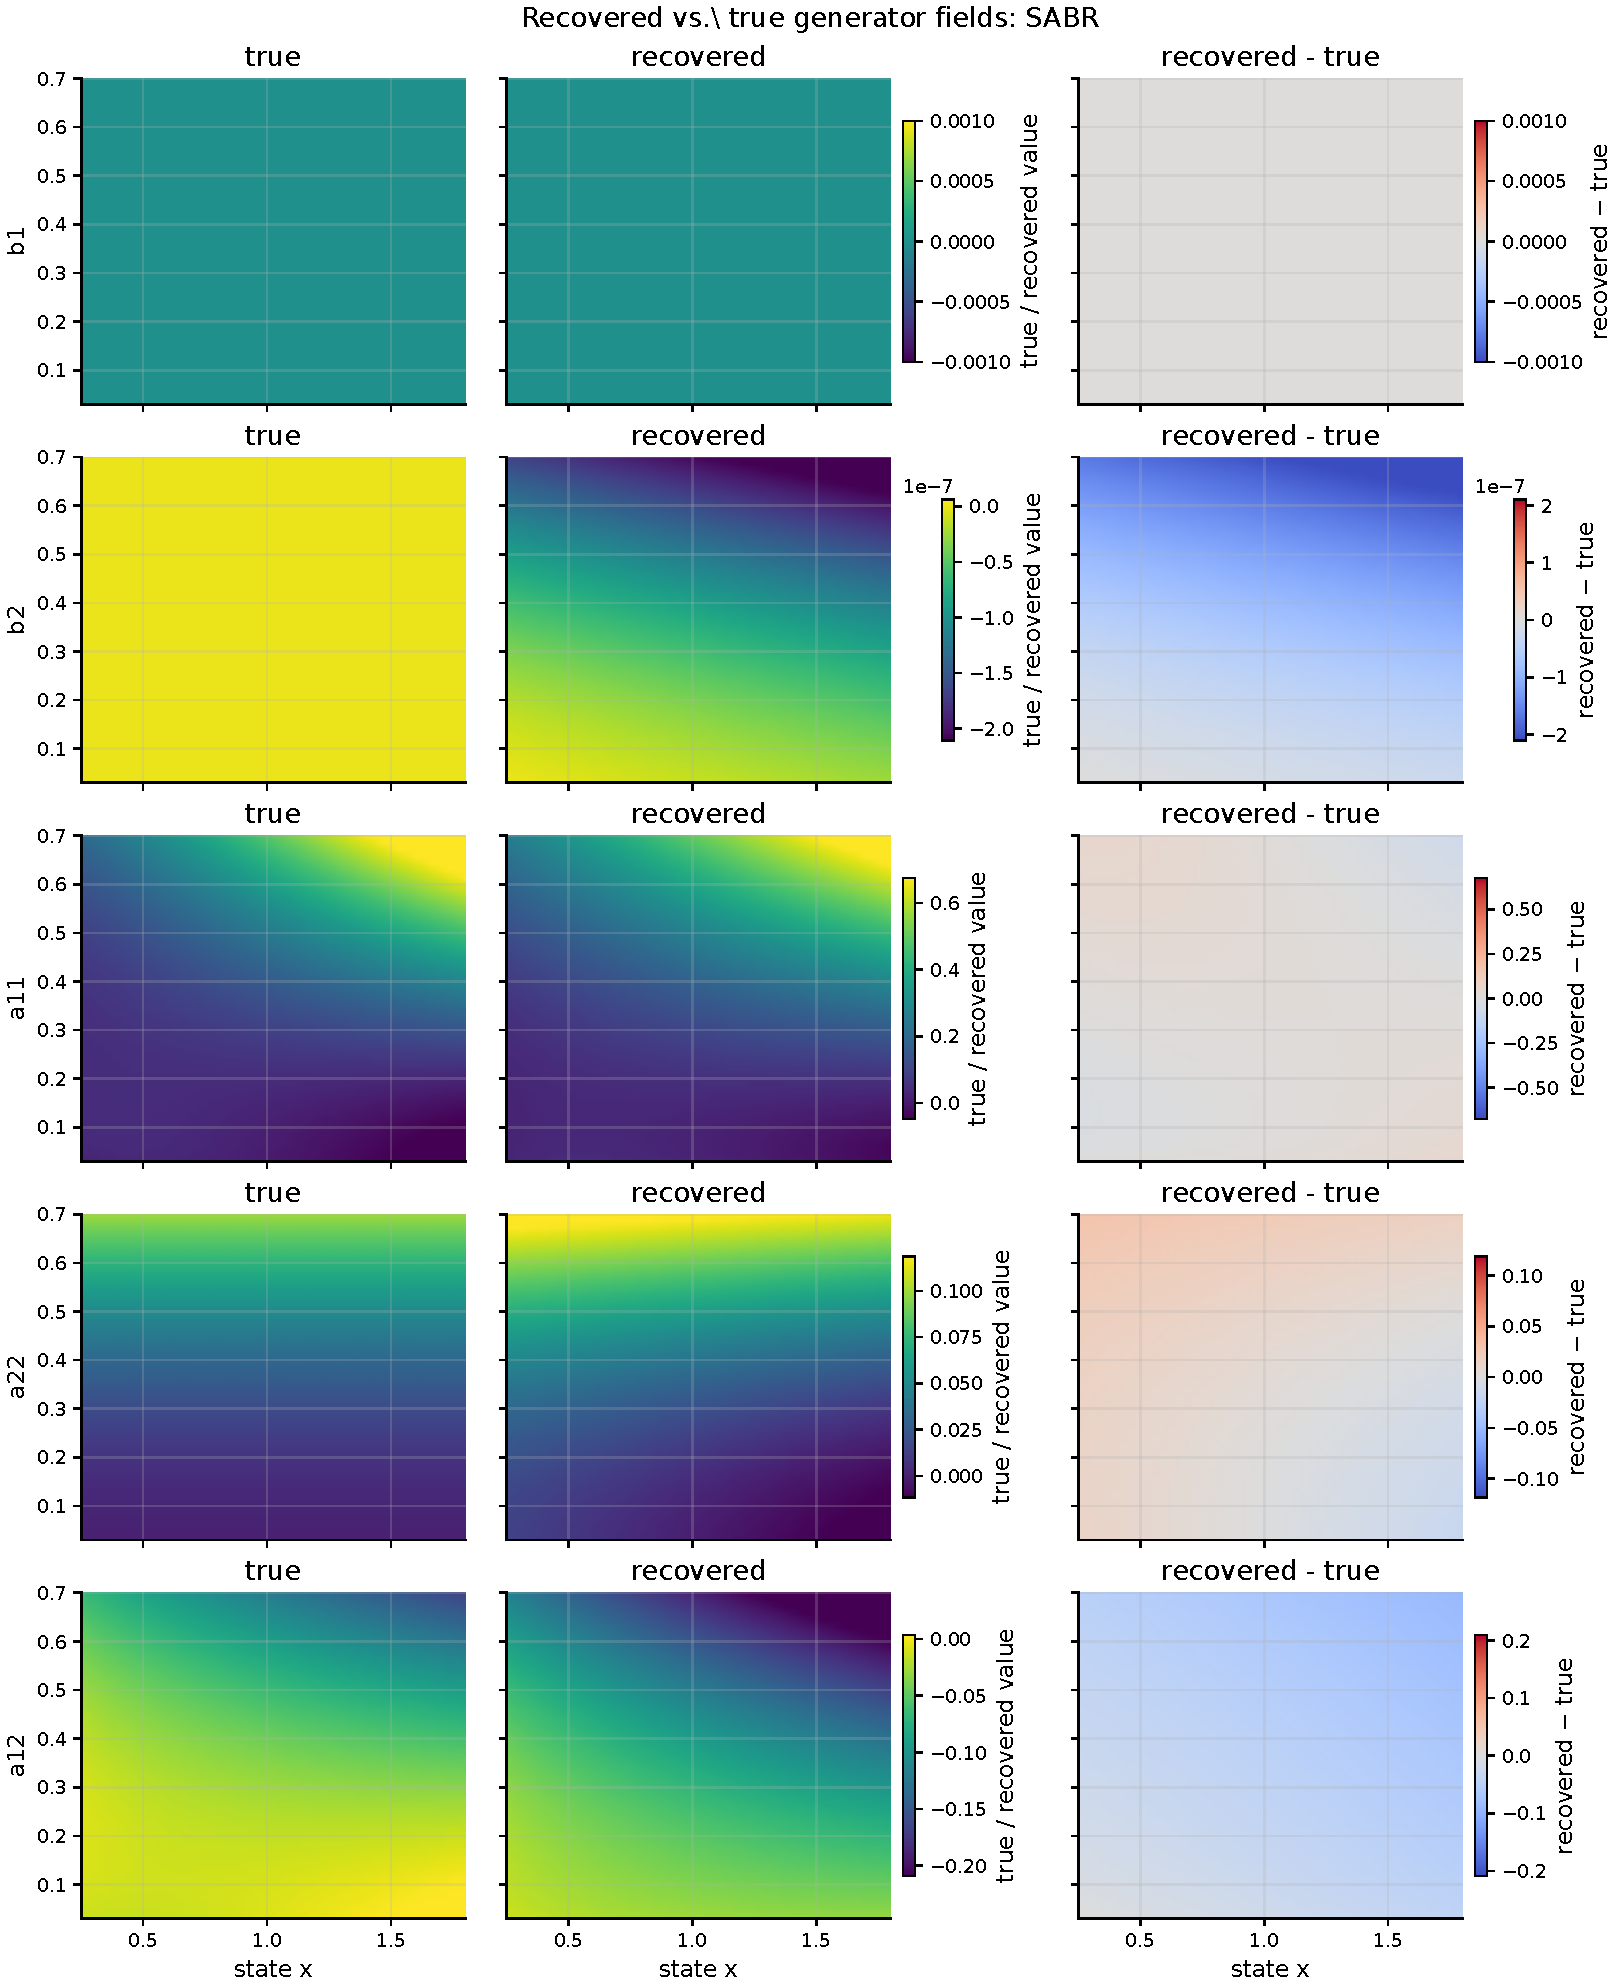
\includegraphics[width=0.86\linewidth]{datasheet_fields_sabr.pdf}
\caption{SABR: recovered vs.\ true generator fields (shared per-field colour scale; error column centred at zero).}\end{figure}
\paragraph{Verdict.} Drift $L^2(\mu)=--$, tensor rel-$L^2=0.195$, $a_{12}$ cosine $0.990$, PSD $1.00$, FP $0$ ($n$ seeds). \textbf{NAMED_NULL}.
\medskip

\subsection{Correlated 2D GBM}\label{sec:v62-gbm-2d}
\paragraph{Context.} Two correlated geometric Brownian motions, the canonical multi-asset price model underlying portfolio and basket-option risk. The asset--asset correlation lives in the off-diagonal $\diff_{12}=\rho\sigma_1\sigma_2 S_1S_2$, which is recovered cleanly; the per-asset drifts $\mu_iS_i$ are dominated by the diffusion and share the low signal-to-noise character of the Heston log-price drift, so the system is reported as a scoped review.
\paragraph{System.} $$\mathrm{d}S_i=\mu_i S_i\,\mathrm{d}t+\sigma_i S_i\mathrm{d}W_i,\ \mathrm{d}W_1\mathrm{d}W_2=\rho\,\mathrm{d}t.$$
\paragraph{Generator.} Two correlated lognormal assets; tensor and $S_1S_2$ leverage recover (cosine $0.997$); the small $\mu_i S_i$ drift is low-SNR. Scoped review.
\paragraph{Recovery.} WG-SINDy recovers the drift at relative $L^2(\mu)=2.492$ and the diffusion tensor at $0.096$ relative error, with off-diagonal (leverage) cosine $0.997$; the off-diagonal yields the price--variance leverage correlation alongside the variance mean-reversion and vol-of-vol. Scoped review (metric gate not met but truth is representable): the truth lies in the library but the metric gate is not met, typically a low-SNR drift component.
\begin{figure}[H]\centering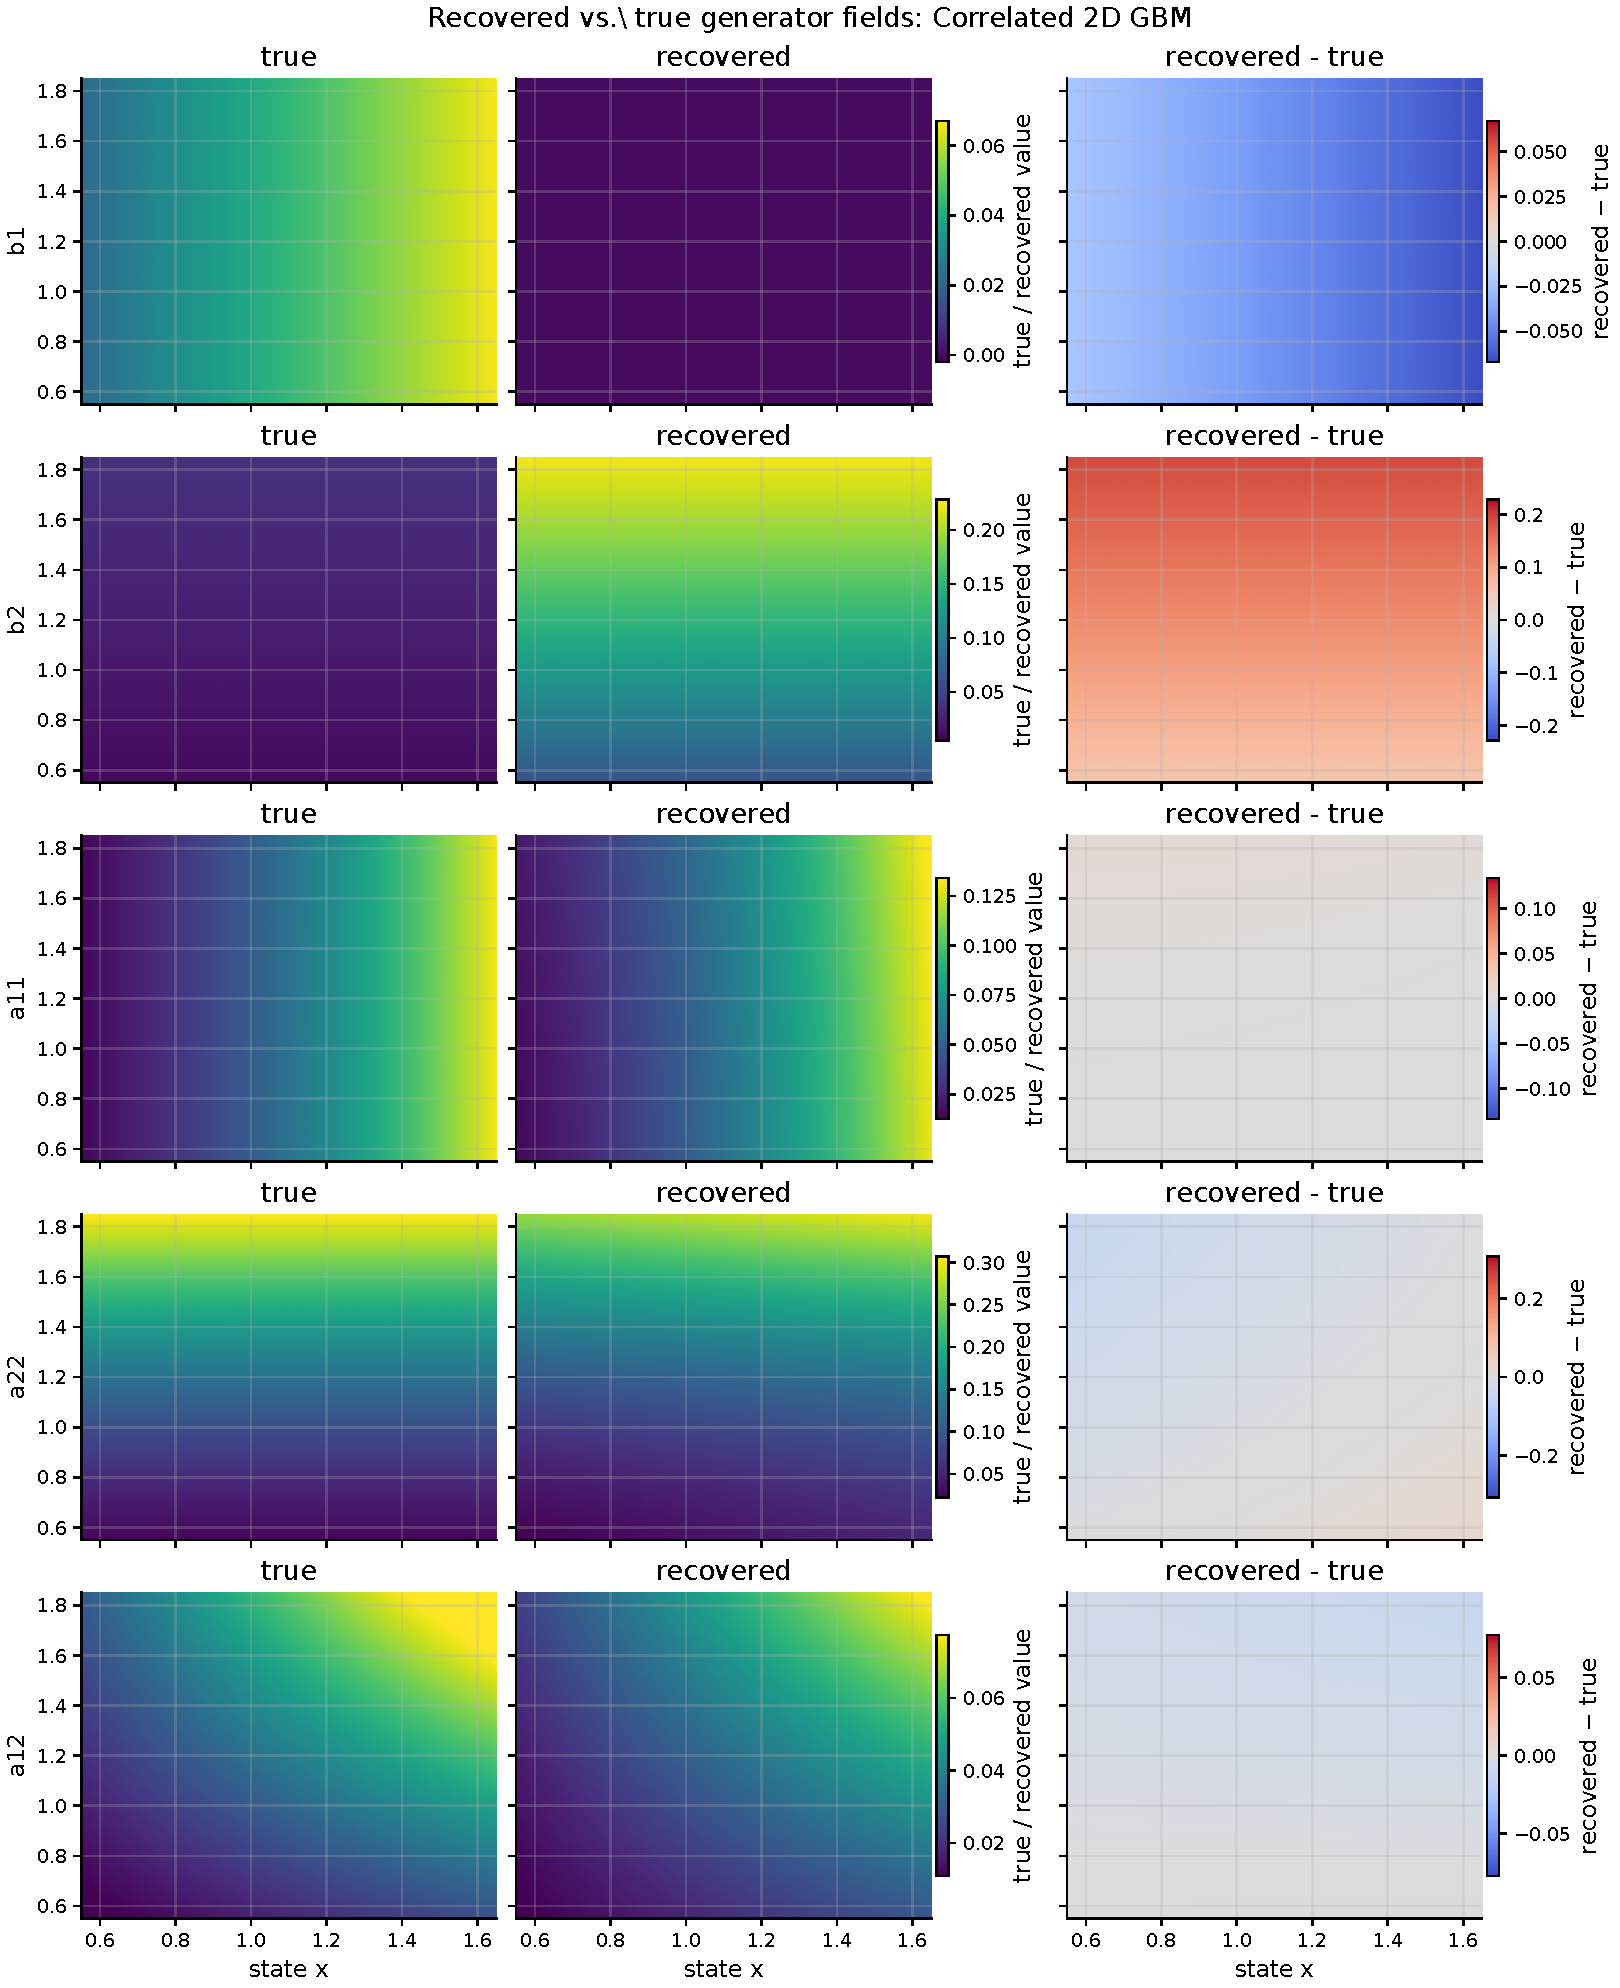
\includegraphics[width=0.86\linewidth]{datasheet_fields_gbm_2d.pdf}
\caption{Correlated 2D GBM: recovered vs.\ true generator fields (shared per-field colour scale; error column centred at zero).}\end{figure}
\paragraph{Verdict.} Drift $L^2(\mu)=2.492$, tensor rel-$L^2=0.096$, $a_{12}$ cosine $0.997$, PSD $1.00$, FP $0$ ($n$ seeds). \textbf{SCOPED_REVIEW}.
\medskip

\subsection{Two-factor Vasicek}\label{sec:v62-two-factor-vasicek}
\paragraph{Context.} A coupled two-factor Vasicek short-rate model, the affine-rates analogue of coupled OU at realistic (micro) scale. Its constant diffusion is so small that relative tensor error becomes a degenerate metric; the affine coupled drift, which is the financially relevant object for term-structure work, is recovered, so it is flagged as a scoped review rather than a pass.
\paragraph{System.} $$\drift=(\kappa_1(\theta_1-X)+c_{12}(Y-\theta_2),\ \kappa_2(\theta_2-Y)+c_{21}(X-\theta_1)).$$
\paragraph{Generator.} Affine coupled short-rate model; constant micro-scale tensor (relative metric degenerate, absolute error small). Scoped review.
\paragraph{Recovery.} WG-SINDy recovers the drift at relative $L^2(\mu)=0.350$ and the diffusion tensor at $1.000$ relative error; the recovered generator gives the relaxation rates and cross-coupling (and, where present, the leverage correlation). Scoped review (metric gate not met but truth is representable): the truth lies in the library but the metric gate is not met, typically a low-SNR drift component.
\begin{figure}[H]\centering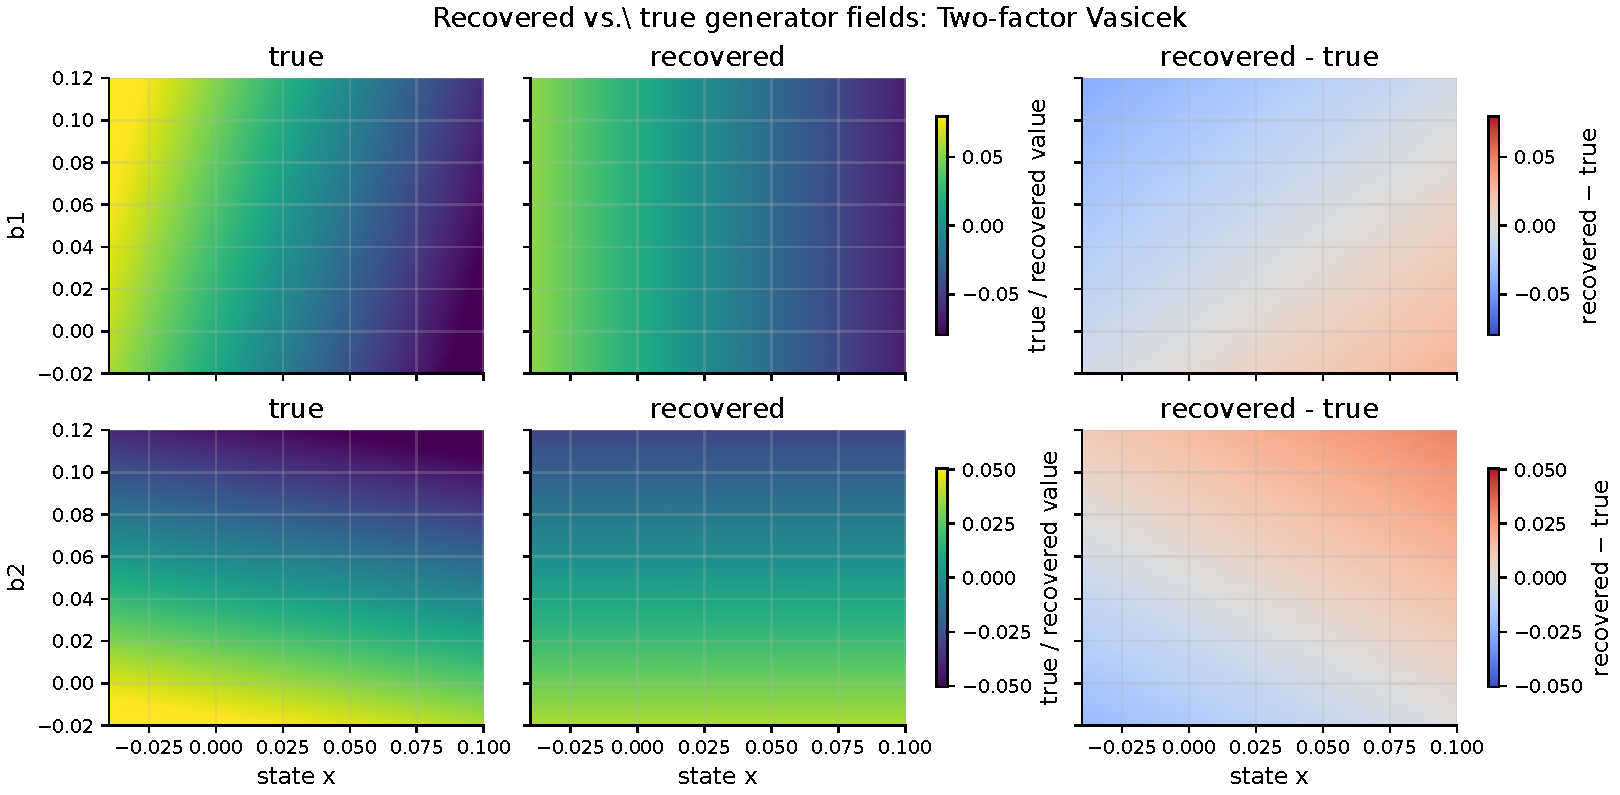
\includegraphics[width=0.86\linewidth]{datasheet_fields_two_factor_vasicek.pdf}
\caption{Two-factor Vasicek: recovered vs.\ true generator fields (shared per-field colour scale; error column centred at zero).}\end{figure}
\paragraph{Verdict.} Drift $L^2(\mu)=0.350$, tensor rel-$L^2=1.000$, $a_{12}$ cosine $n/a$, PSD $1.00$, FP $0$ ($n$ seeds). \textbf{SCOPED_REVIEW}.
\medskip
}{}
\IfFileExists{ds_limitcycle.tex}{% Auto-generated tight datasheets. Coefficients live in the aggregate R32 table. Source: results/v10/coeff_recovery_R32.csv
\paragraph{Stochastic limit cycles}\;

\subsection{Van der Pol}\label{sec:v62-van-der-pol}
\paragraph{Context.} The Van der Pol oscillator is the archetype of a self-sustained relaxation oscillation, originating in electronic circuits and reused for cardiac and neural rhythms. It is the first demonstration that the weak-form recovery extends to limit-cycle dynamics, a regime absent from the one-dimensional benchmarks: trajectories concentrate on a closed attractor, so the cubic nonlinear-damping term $-\mu x^2y$ is recovered from dense repeated traversal of the cycle even though the rest of phase space is sparsely sampled.
\paragraph{System.} $$\mathrm{d}X=Y\,\mathrm{d}t,\ \mathrm{d}Y=(\mu(1-X^2)Y-X)\mathrm{d}t+\sigma\mathrm{d}W,\ \mu=1.2.$$
\paragraph{Generator.} Self-sustained limit cycle; the cubic cross term $-\mu x^2y$ is the nonlinear damping. Tight repeated sampling on the cycle aids recovery.
\paragraph{Recovery.} WG-SINDy recovers the drift at relative $L^2(\mu)=0.066$ and the diffusion tensor at $0.040$ relative error; the recovered drift reproduces the limit-cycle geometry and the oscillation frequency. The active symbolic terms are recovered at selection rate one with no false positives; weaker secondary terms carry a lower selection rate.
\begin{figure}[H]\centering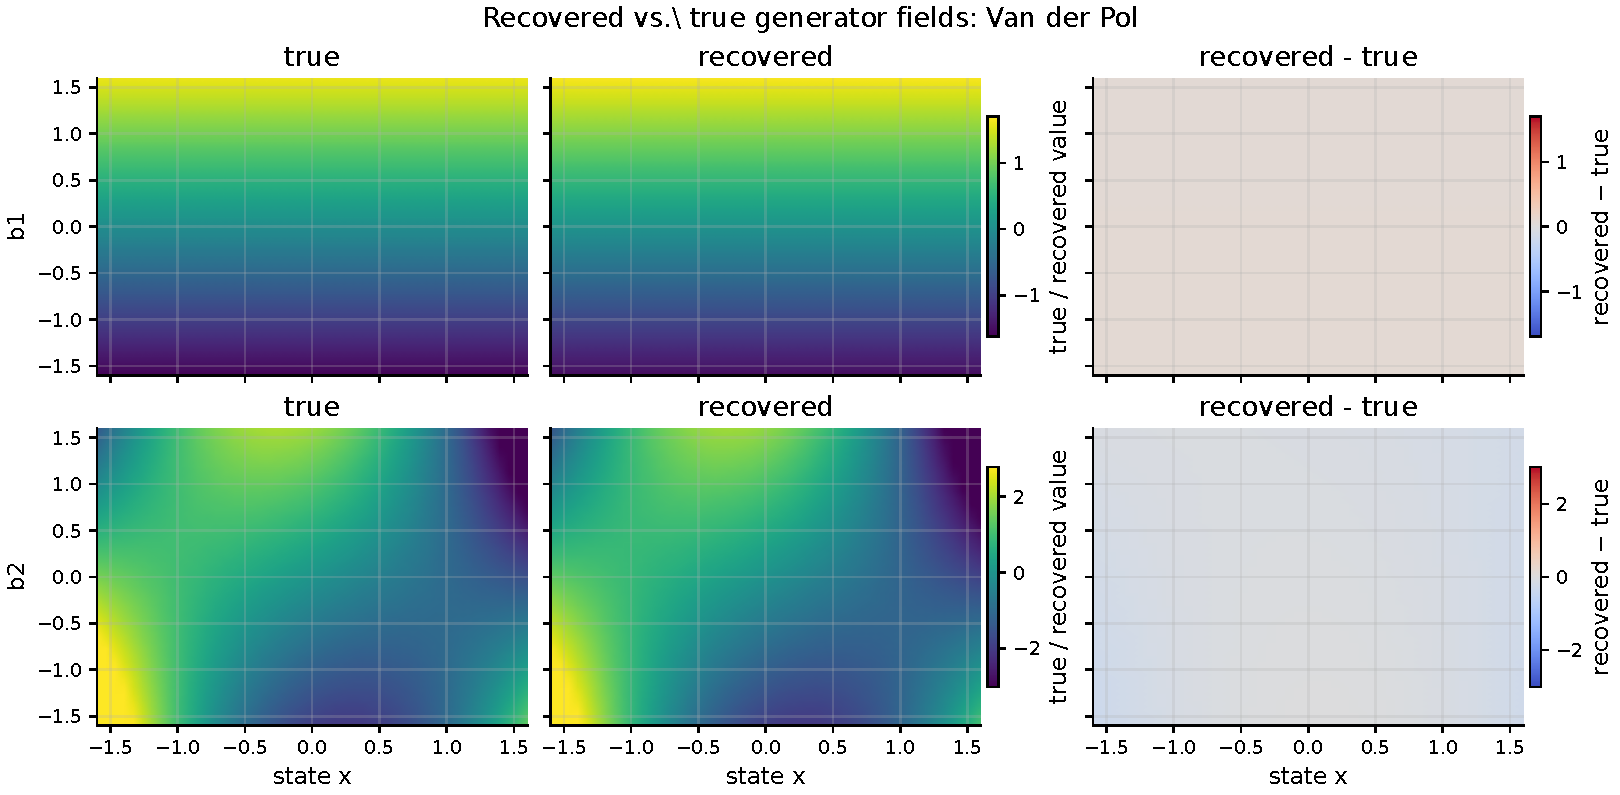
\includegraphics[width=0.86\linewidth]{datasheet_fields_van_der_pol.pdf}
\caption{Van der Pol: recovered vs.\ true generator fields (shared per-field colour scale; error column centred at zero).}\end{figure}
\paragraph{Verdict.} Drift $L^2(\mu)=0.066$, tensor rel-$L^2=0.040$, $a_{12}$ cosine $n/a$, PSD $1.00$, FP $0$ ($n$ seeds). \textbf{PASS}.
\medskip

\subsection{Stuart--Landau}\label{sec:v62-stuart-landau}
\paragraph{Context.} The Stuart--Landau equation is the universal normal form of a supercritical Hopf bifurcation, describing the generic onset of oscillation. It combines cubic radial damping with a pure rotation, so it simultaneously exercises the nonlinear-drift and circulation capabilities; its rotational symmetry gives uniform angular coverage of the limit cycle and yields the cleanest oscillatory recovery in the study.
\paragraph{System.} $$\drift=((\lambda-r^2)X-\omega Y,\ \omega X+(\lambda-r^2)Y),\ r^2=X^2+Y^2.$$
\paragraph{Generator.} Supercritical Hopf normal form: cubic radial damping ($x^3,xy^2,x^2y,y^3$) plus linear rotation $\pm\omega$; rotation-symmetric sampling gives clean recovery.
\paragraph{Recovery.} WG-SINDy recovers the drift at relative $L^2(\mu)=0.126$ and the diffusion tensor at $0.018$ relative error; the recovered drift reproduces the limit-cycle geometry and the oscillation frequency. The active symbolic terms are recovered at selection rate one with no false positives; weaker secondary terms carry a lower selection rate.
\begin{figure}[H]\centering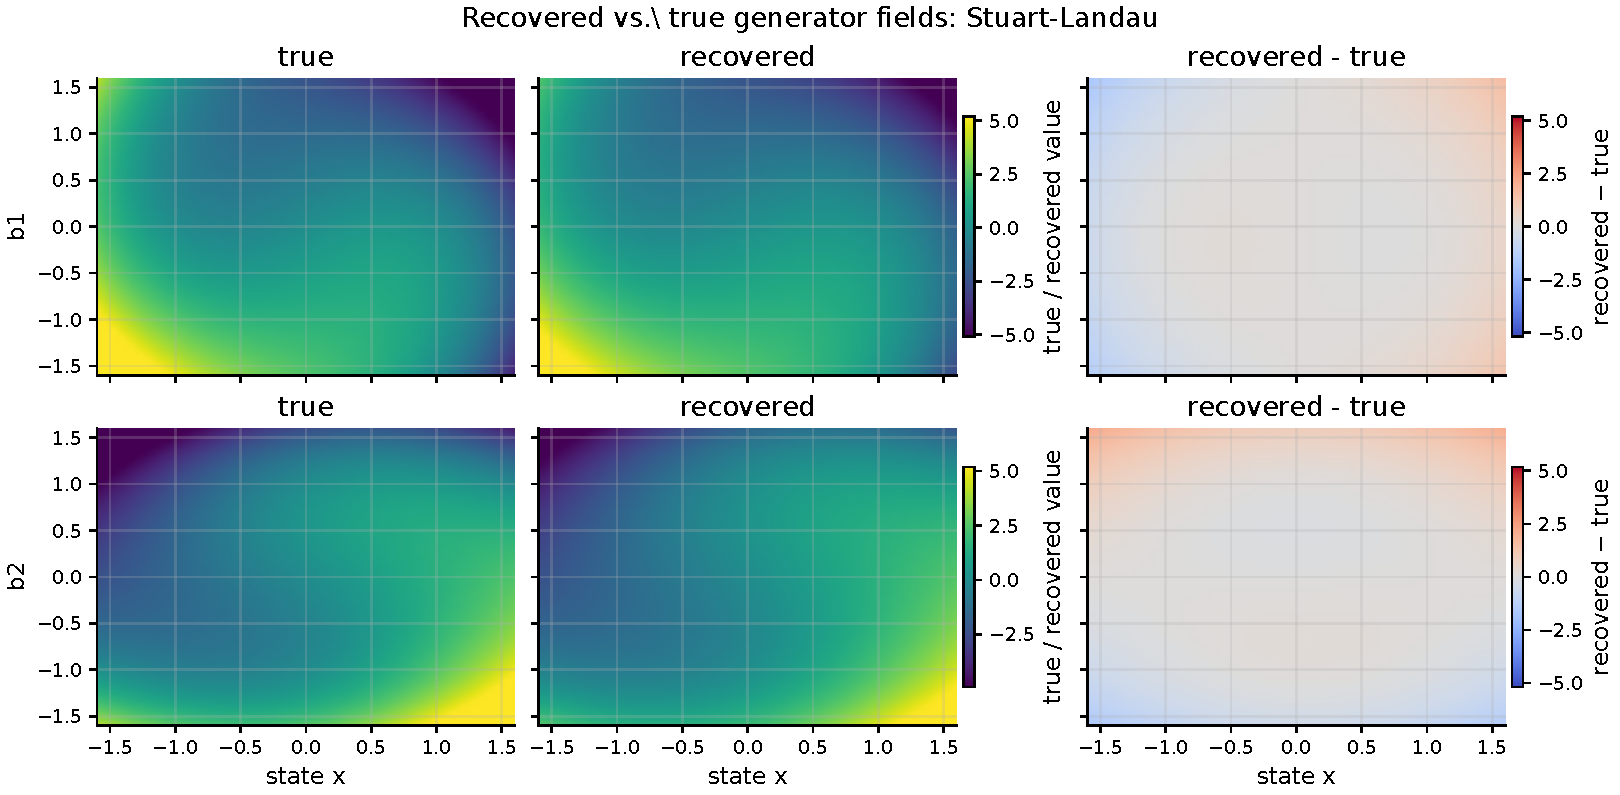
\includegraphics[width=0.86\linewidth]{datasheet_fields_stuart_landau.pdf}
\caption{Stuart--Landau: recovered vs.\ true generator fields (shared per-field colour scale; error column centred at zero).}\end{figure}
\paragraph{Verdict.} Drift $L^2(\mu)=0.126$, tensor rel-$L^2=0.018$, $a_{12}$ cosine $n/a$, PSD $1.00$, FP $0$ ($n$ seeds). \textbf{PASS}.
\medskip

\subsection{Brusselator}\label{sec:v62-brusselator}
\paragraph{Context.} The Brusselator is a classic model of an autocatalytic chemical oscillator and a staple of reaction--diffusion theory. Its drift is polynomial with a shared autocatalytic $x^2y$ term of opposite sign in the two species; recovering this mass-action structure from data demonstrates that the method discovers chemically interpretable kinetics, not merely abstract polynomials.
\paragraph{System.} $$\drift=(A-(B+1)X+X^2Y,\ BX-X^2Y),\ A=1,B=2.6,\ \diff=0.0144 I.$$
\paragraph{Generator.} Chemical limit cycle with the autocatalytic $x^2y$ term shared (opposite signs) across components.
\paragraph{Recovery.} WG-SINDy recovers the drift at relative $L^2(\mu)=0.013$ and the diffusion tensor at $0.067$ relative error; the recovered drift reproduces the limit-cycle geometry and the oscillation frequency. The active symbolic terms are recovered at selection rate one with no false positives; weaker secondary terms carry a lower selection rate.
\begin{figure}[H]\centering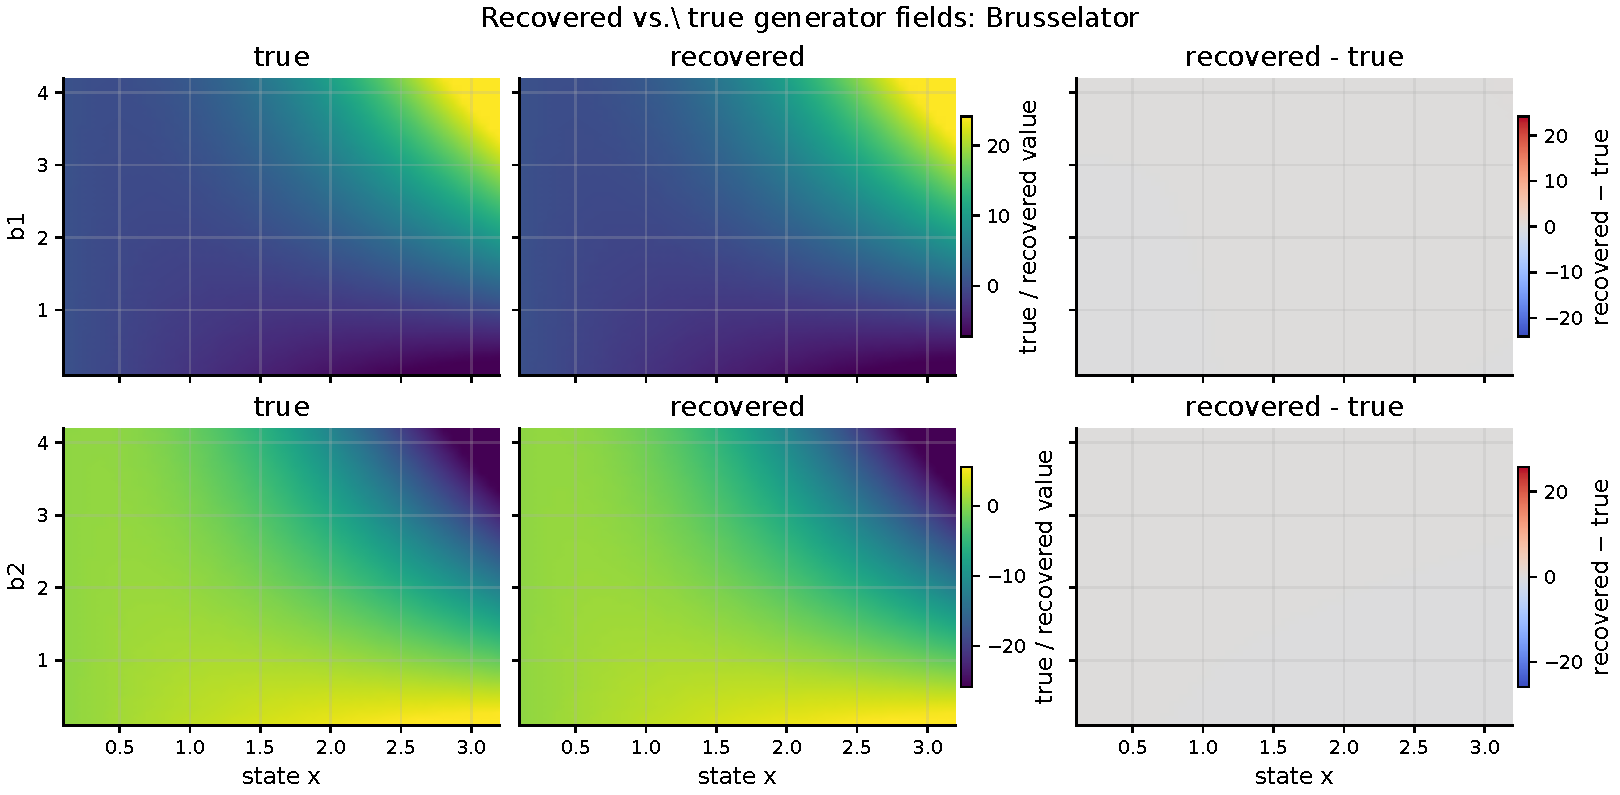
\includegraphics[width=0.86\linewidth]{datasheet_fields_brusselator.pdf}
\caption{Brusselator: recovered vs.\ true generator fields (shared per-field colour scale; error column centred at zero).}\end{figure}
\paragraph{Verdict.} Drift $L^2(\mu)=0.013$, tensor rel-$L^2=0.067$, $a_{12}$ cosine $n/a$, PSD $1.00$, FP $0$ ($n$ seeds). \textbf{PASS}.
\medskip
}{}
\IfFileExists{ds_limits.tex}{% Auto-generated tight datasheets. Coefficients live in the aggregate R32 table. Source: results/v10/coeff_recovery_R32.csv
\paragraph{Named limits (reported, not hidden)}\;

\subsection{Near-singular tensor}\label{sec:v62-near-singular}
\paragraph{Context.} A deliberate stress of the positive-semidefinite boundary: the off-diagonal is pushed to $0.95\sqrt{\diff_{11}\diff_{22}}$, so the two noise directions are nearly collinear and the tensor is almost rank-deficient. It marks the edge of identifiability for the diffusion tensor and is reported as a named limit, where the Cholesky parametrisation still guarantees a valid covariance but the magnitude of the off-diagonal is no longer well determined by finite data.
\paragraph{System.} $$\drift=-X,\ \diff_{12}=0.95\sqrt{\diff_{11}\diff_{22}}.$$
\paragraph{Generator.} Off-diagonal pushed to the PSD boundary ($\det\diff\to0$): the two noise directions are nearly collinear, so the off-diagonal is ill-conditioned. Named limit.
\paragraph{Recovery.} WG-SINDy recovers the drift at relative $L^2(\mu)=0.870$ and the diffusion tensor at $1.505$ relative error, with off-diagonal (leverage) cosine $0.724$; the recovered diffusion tensor is a position-dependent field giving the local fluctuation amplitude and relaxation. This is a named limit (fragile physics or identifiability limit): recovery fails for a physical or identifiability reason (library incompleteness, low signal-to-noise, degeneracy, or coverage), not an estimator defect.
\begin{figure}[H]\centering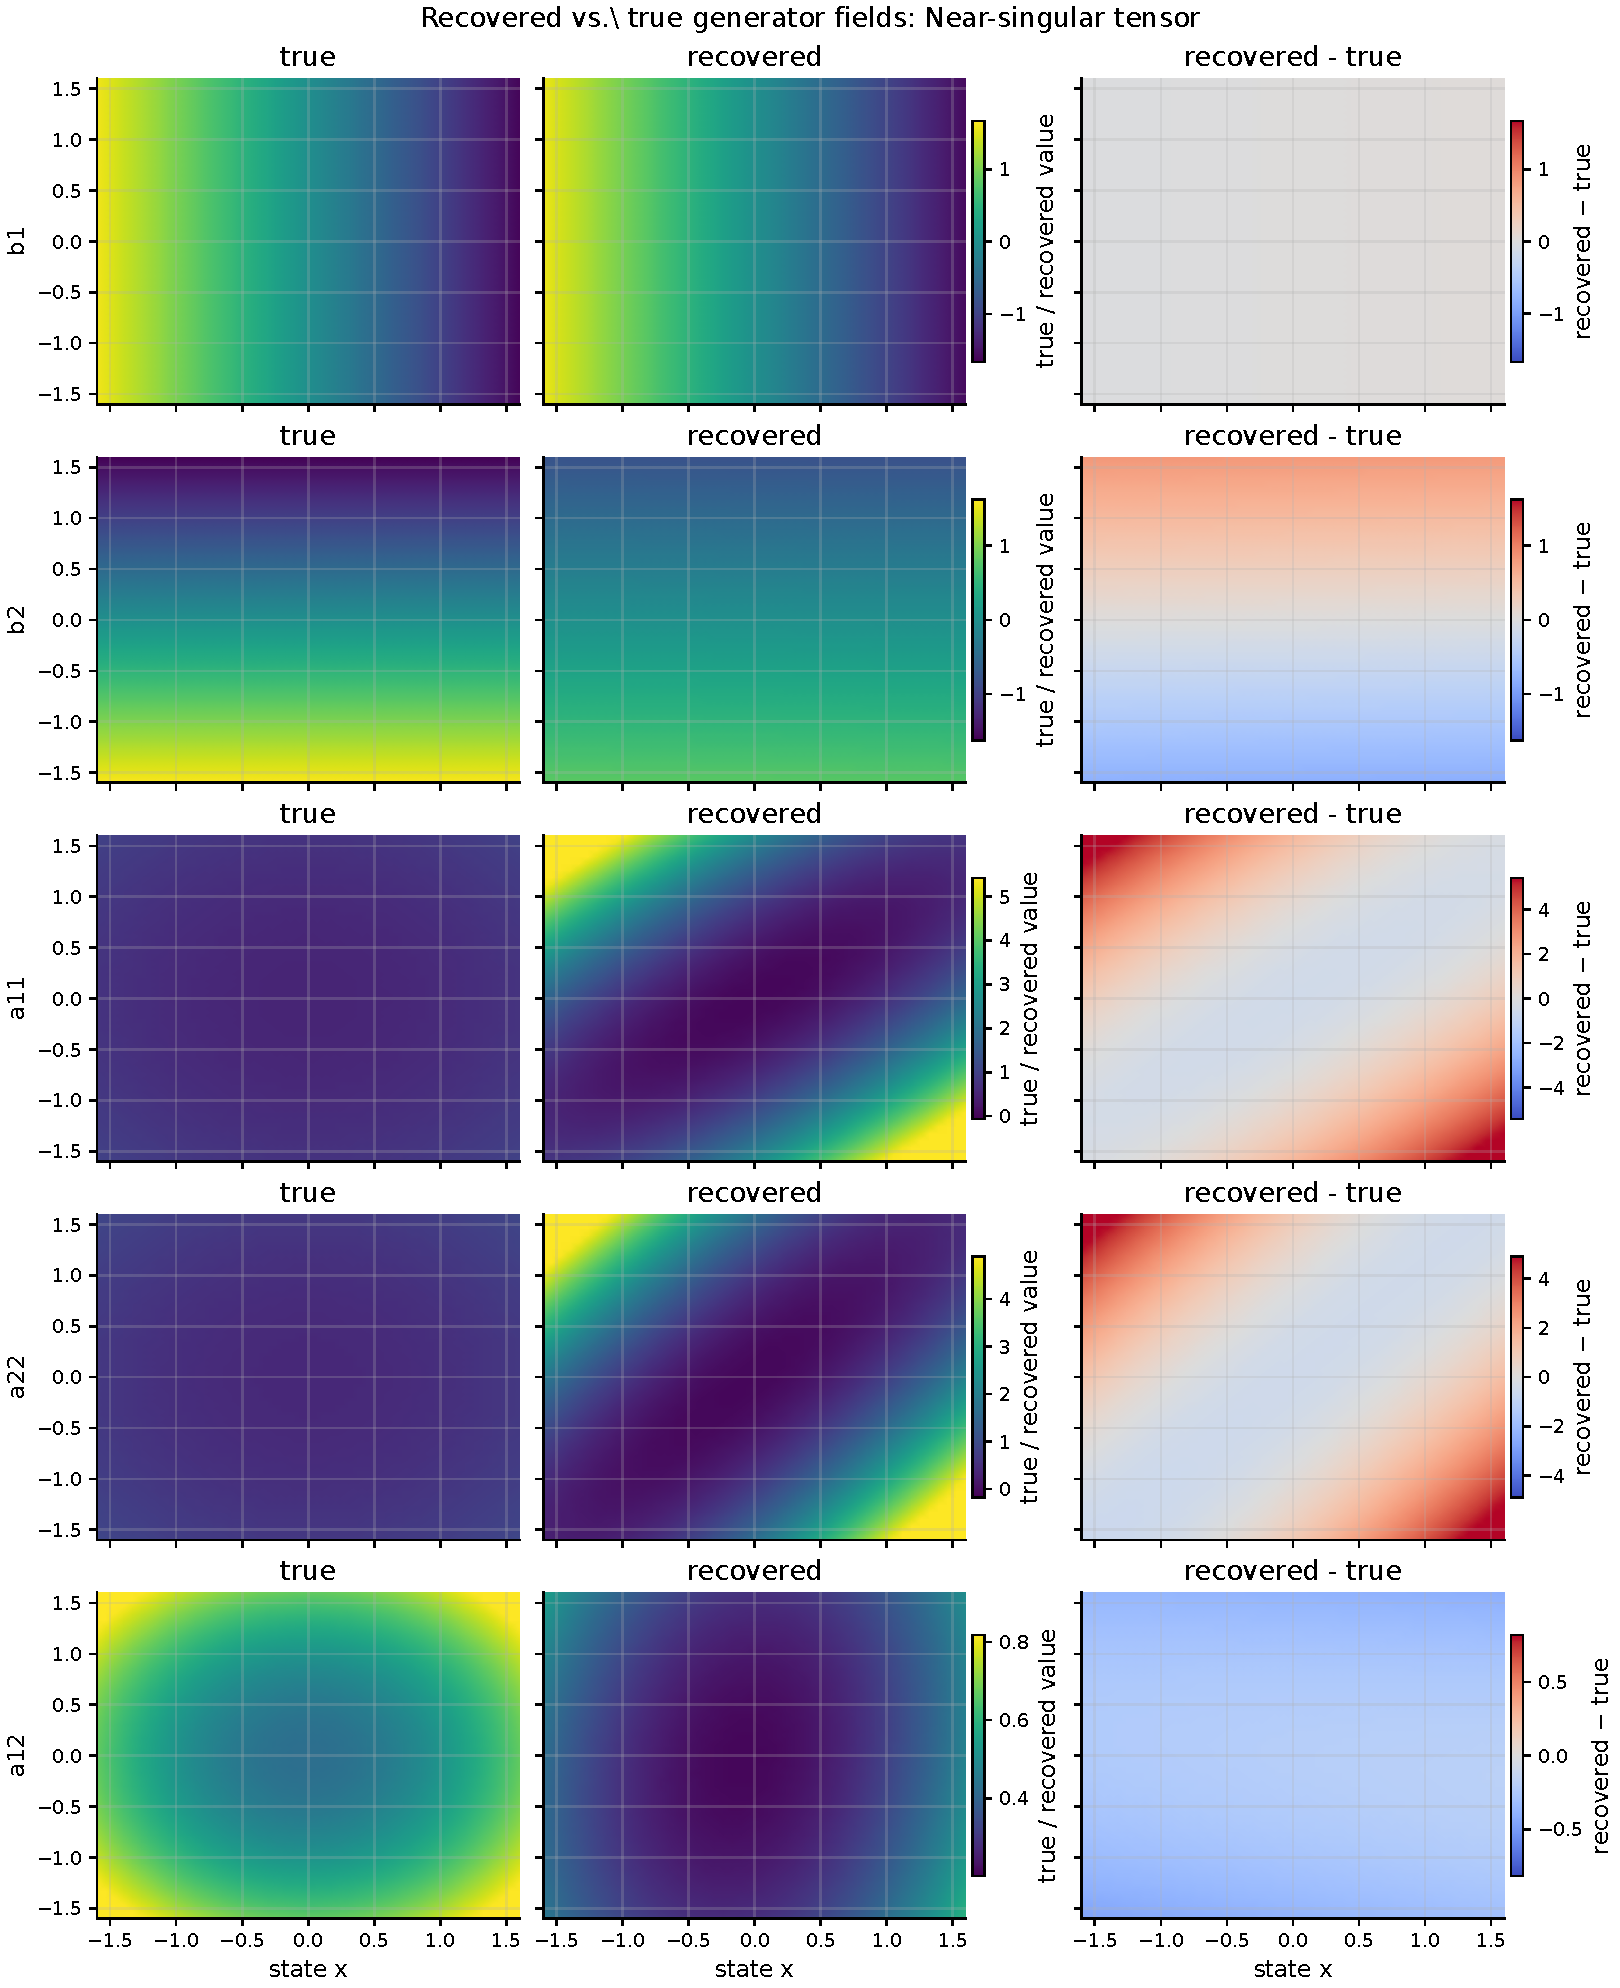
\includegraphics[width=0.86\linewidth]{datasheet_fields_near_singular.pdf}
\caption{Near-singular tensor: recovered vs.\ true generator fields (shared per-field colour scale; error column centred at zero).}\end{figure}
\paragraph{Verdict.} Drift $L^2(\mu)=0.870$, tensor rel-$L^2=1.505$, $a_{12}$ cosine $0.724$, PSD $1.00$, FP $0$ ($n$ seeds). \textbf{NAMED_NULL}.
\medskip

\subsection{Underdamped Langevin}\label{sec:v62-underdamped-langevin}
\paragraph{Context.} Underdamped (kinetic) Langevin dynamics in position--momentum form, ubiquitous in molecular dynamics and sampling. Only the momentum coordinate is driven by noise, so the diffusion tensor is rank-one with structural zeros in $\diff_{11}$ and $\diff_{12}$, a degenerate target retained as a named limit to show how the method behaves when one direction carries no direct fluctuation.
\paragraph{System.} $$\mathrm{d}Q=P\,\mathrm{d}t,\ \mathrm{d}P=(-\gamma P-(Q^3-Q))\mathrm{d}t+\sigma\mathrm{d}W.$$
\paragraph{Generator.} Degenerate rank-1 diffusion ($\diff_{11}=\diff_{12}=0$): one coordinate carries no direct noise. Named limit.
\paragraph{Recovery.} WG-SINDy recovers the drift at relative $L^2(\mu)=0.157$ and the diffusion tensor at $0.563$ relative error; this system is reported as a named limit. This is a named limit (fragile physics or identifiability limit): recovery fails for a physical or identifiability reason (library incompleteness, low signal-to-noise, degeneracy, or coverage), not an estimator defect.
\begin{figure}[H]\centering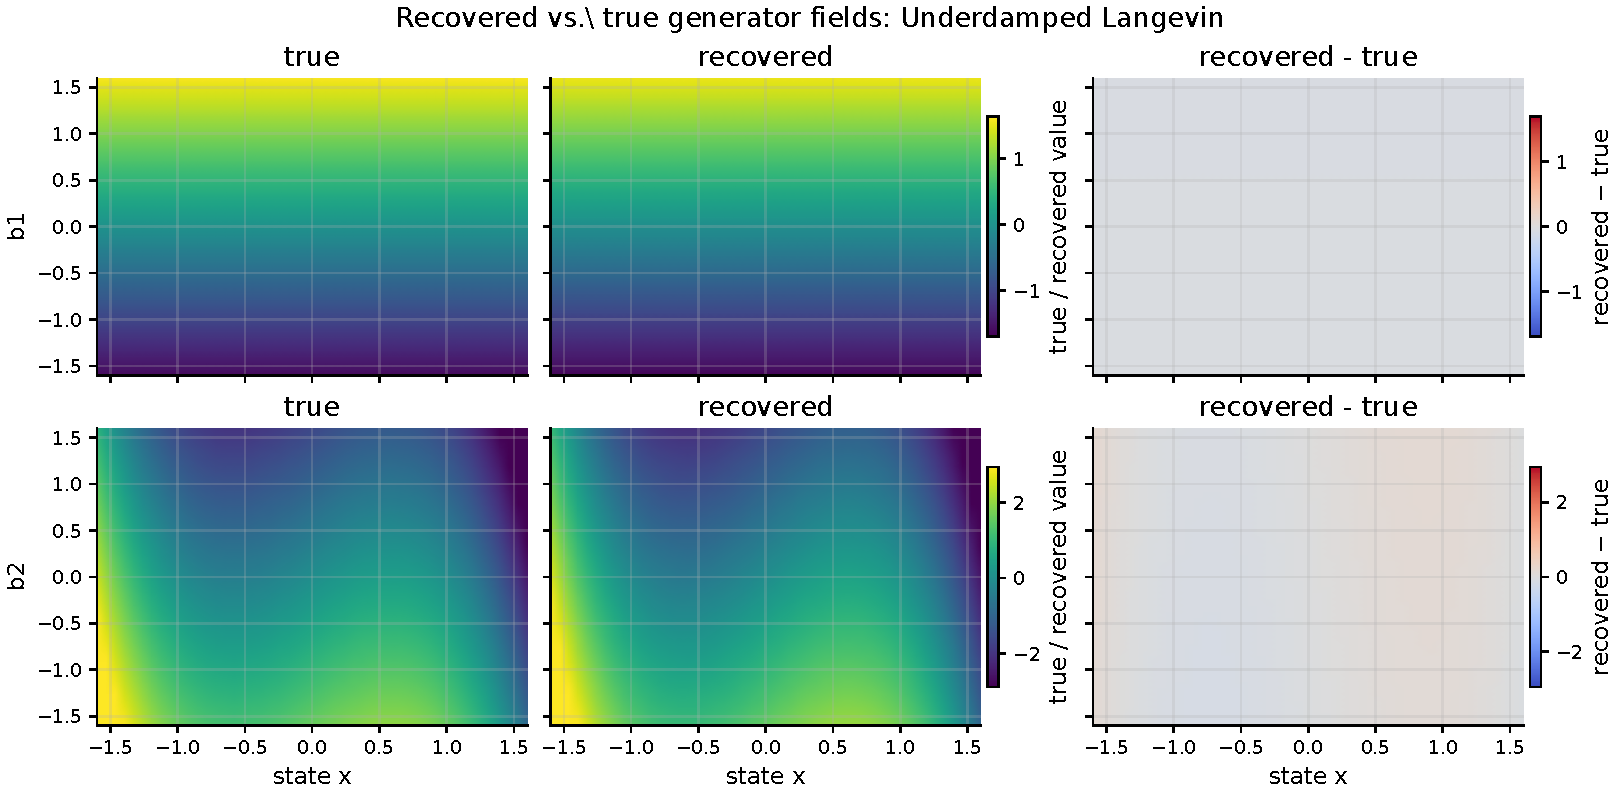
\includegraphics[width=0.86\linewidth]{datasheet_fields_underdamped_langevin.pdf}
\caption{Underdamped Langevin: recovered vs.\ true generator fields (shared per-field colour scale; error column centred at zero).}\end{figure}
\paragraph{Verdict.} Drift $L^2(\mu)=0.157$, tensor rel-$L^2=0.563$, $a_{12}$ cosine $n/a$, PSD $1.00$, FP $0$ ($n$ seeds). \textbf{NAMED_NULL}.
\medskip

\subsection{Near-boundary Heston}\label{sec:v62-near-boundary-heston}
\paragraph{Context.} A Heston regime that violates the Feller condition, so the variance process spends substantial mass near zero. It probes the estimator at an absorbing/reflecting boundary, where the square-root diffusion is singular and kernel support is truncated; the tensor and leverage survive but the drift degrades, a named boundary limit rather than an estimator defect.
\paragraph{System.} $$\text{Log-Heston with }2\kappa\theta<\xi^2\ (\text{Feller-violating}).$$
\paragraph{Generator.} Variance spends mass near $v\to0$; boundary bias degrades drift recovery. Tensor/leverage survive. Named limit.
\paragraph{Recovery.} WG-SINDy recovers the drift at relative $L^2(\mu)=1.413$ and the diffusion tensor at $0.267$ relative error, with off-diagonal (leverage) cosine $0.982$; this system is reported as a named limit. This is a named limit (fragile physics or identifiability limit): recovery fails for a physical or identifiability reason (library incompleteness, low signal-to-noise, degeneracy, or coverage), not an estimator defect.
\begin{figure}[H]\centering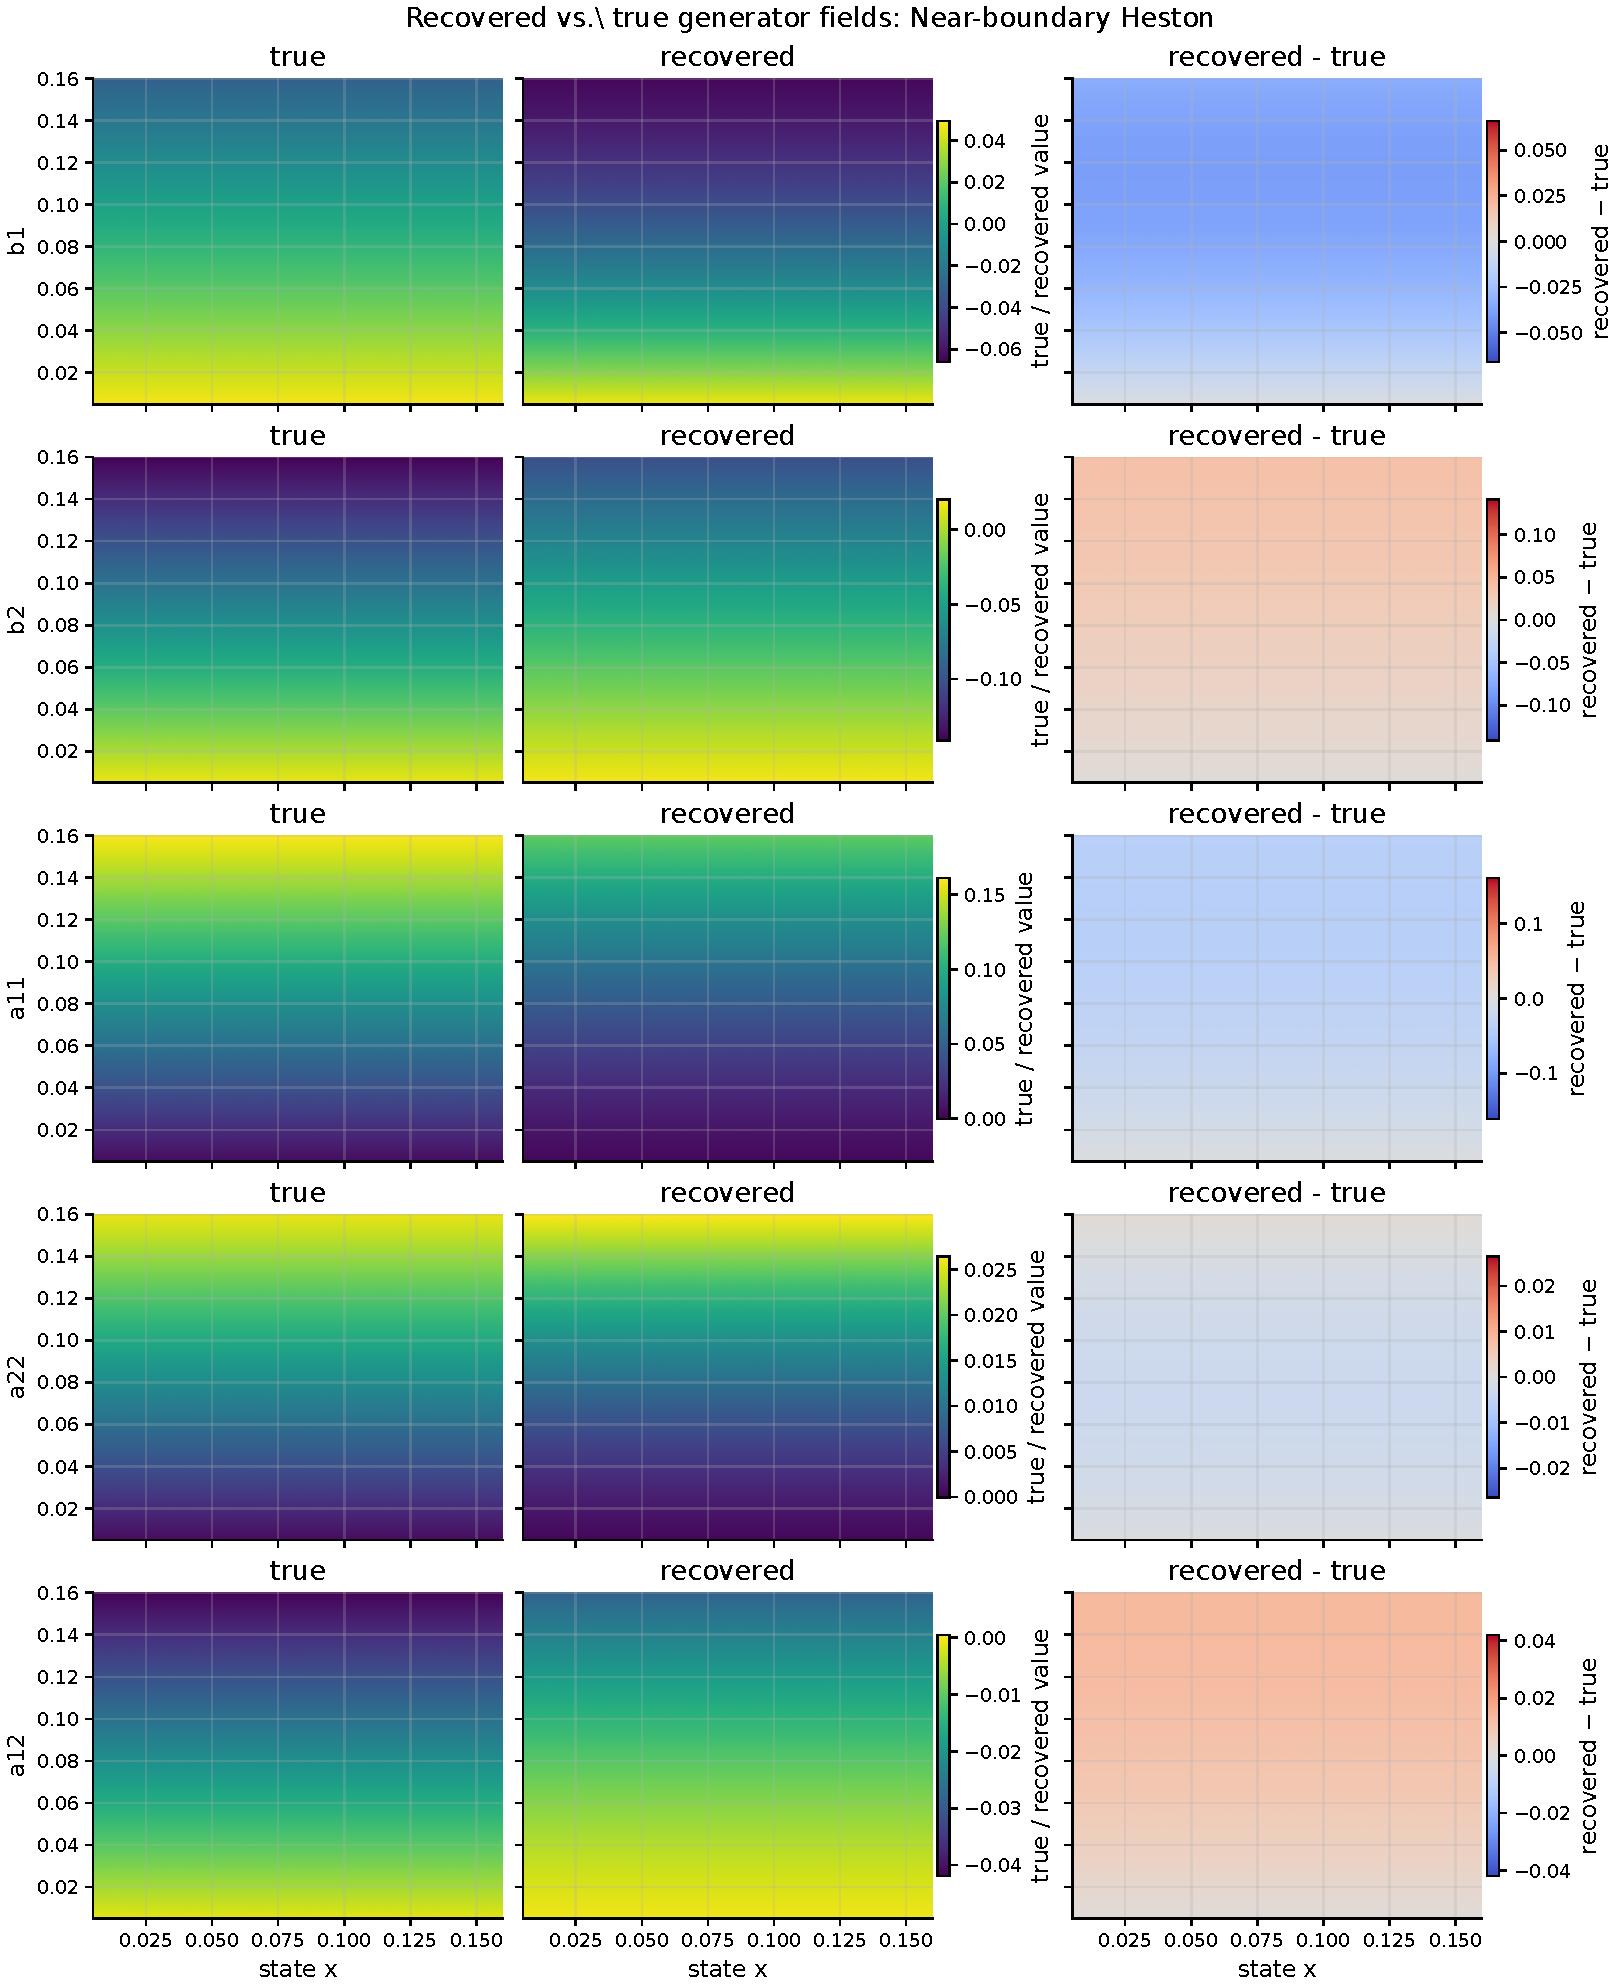
\includegraphics[width=0.86\linewidth]{datasheet_fields_near_boundary_heston.pdf}
\caption{Near-boundary Heston: recovered vs.\ true generator fields (shared per-field colour scale; error column centred at zero).}\end{figure}
\paragraph{Verdict.} Drift $L^2(\mu)=1.413$, tensor rel-$L^2=0.267$, $a_{12}$ cosine $0.982$, PSD $1.00$, FP $0$ ($n$ seeds). \textbf{NAMED_NULL}.
\medskip

\subsection{Non-polynomial drift}\label{sec:v62-nonpoly-drift}
\paragraph{Context.} A system with genuinely non-polynomial (trigonometric) drift, included to make the library-completeness requirement explicit. With a polynomial dictionary it fails by construction; with the trigonometric library it is recovered. It is the clean demonstration that, like every dictionary-based identification method, recovery is conditional on the true terms lying in the chosen feature set.
\paragraph{System.} $$\drift=(-X+\sin Y,\ -Y+\cos X),\ \diff=0.49 I.$$
\paragraph{Generator.} Trigonometric drift: recovered only with the trig library G; a representability limit for any polynomial dictionary. Named limit.
\paragraph{Recovery.} WG-SINDy recovers the drift at relative $L^2(\mu)=0.210$ and the diffusion tensor at $0.037$ relative error; this system is reported as a named limit. This is a named limit (registry declared failure or stress case): recovery fails for a physical or identifiability reason (library incompleteness, low signal-to-noise, degeneracy, or coverage), not an estimator defect.
\begin{figure}[H]\centering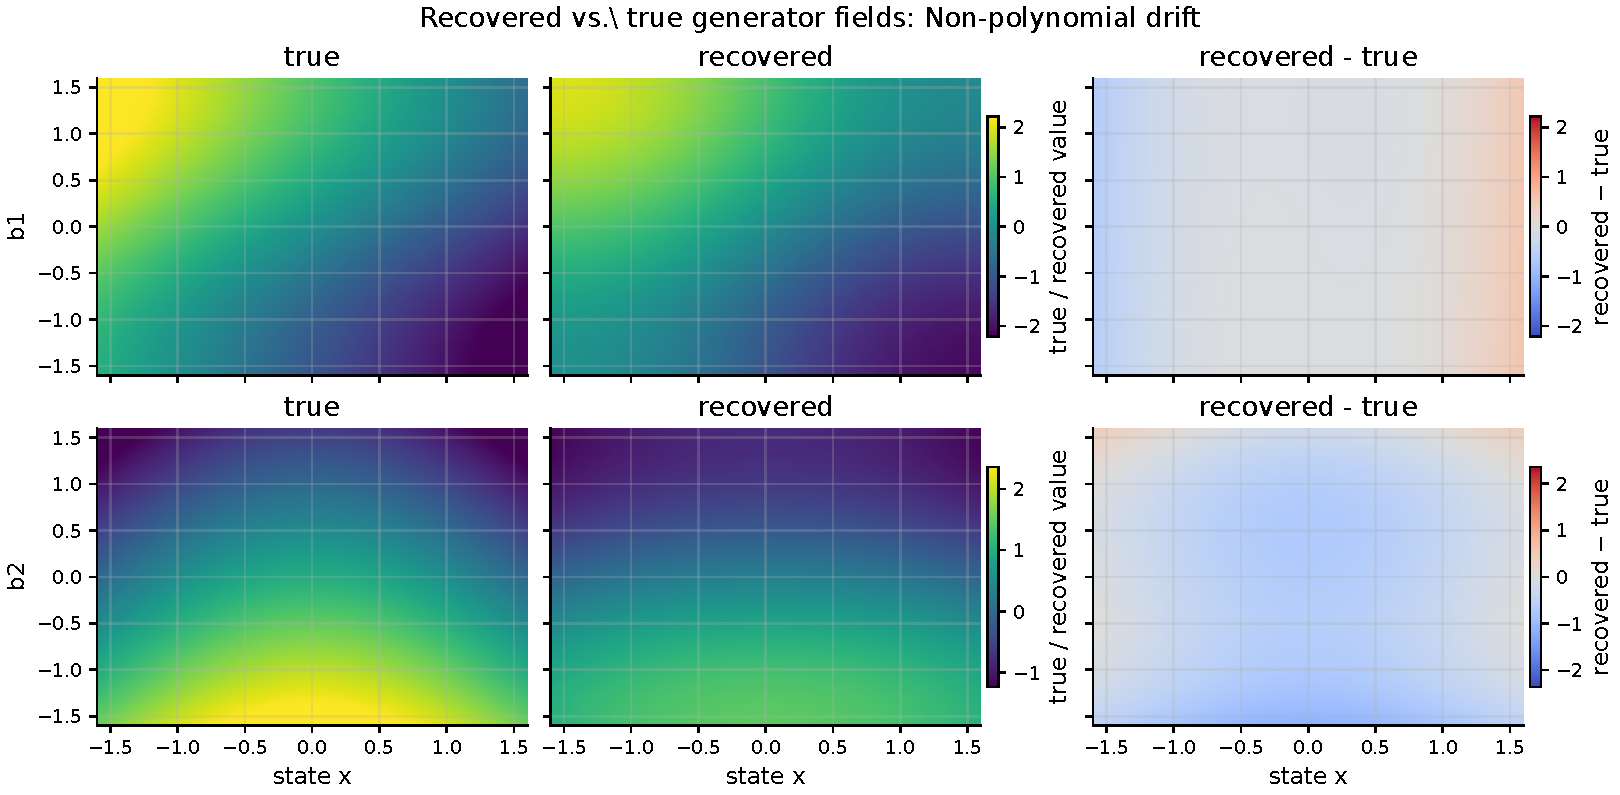
\includegraphics[width=0.86\linewidth]{datasheet_fields_nonpoly_drift.pdf}
\caption{Non-polynomial drift: recovered vs.\ true generator fields (shared per-field colour scale; error column centred at zero).}\end{figure}
\paragraph{Verdict.} Drift $L^2(\mu)=0.210$, tensor rel-$L^2=0.037$, $a_{12}$ cosine $n/a$, PSD $1.00$, FP $0$ ($n$ seeds). \textbf{NAMED_NULL}.
\medskip

\subsection{Bad coverage}\label{sec:v62-bad-coverage}
\paragraph{Context.} A coverage-failure stress case: a rotational OU sampled from trajectories confined to a small region with a short horizon. With the state space under-explored the design matrix becomes rank-deficient, and recovery fails for a data-geometry reason rather than a modelling one, a named limit that delineates the coverage condition the consistency theory requires.
\paragraph{System.} $$\text{Rotational OU, trajectories confined near }(2,2).$$
\paragraph{Generator.} Clustered initial condition and short horizon leave the state space under-covered, so the design is rank-deficient. Named limit.
\paragraph{Recovery.} WG-SINDy recovers the drift at relative $L^2(\mu)=0.815$ and the diffusion tensor at $0.784$ relative error; this system is reported as a named limit. This is a named limit (registry declared failure or stress case): recovery fails for a physical or identifiability reason (library incompleteness, low signal-to-noise, degeneracy, or coverage), not an estimator defect.
\begin{figure}[H]\centering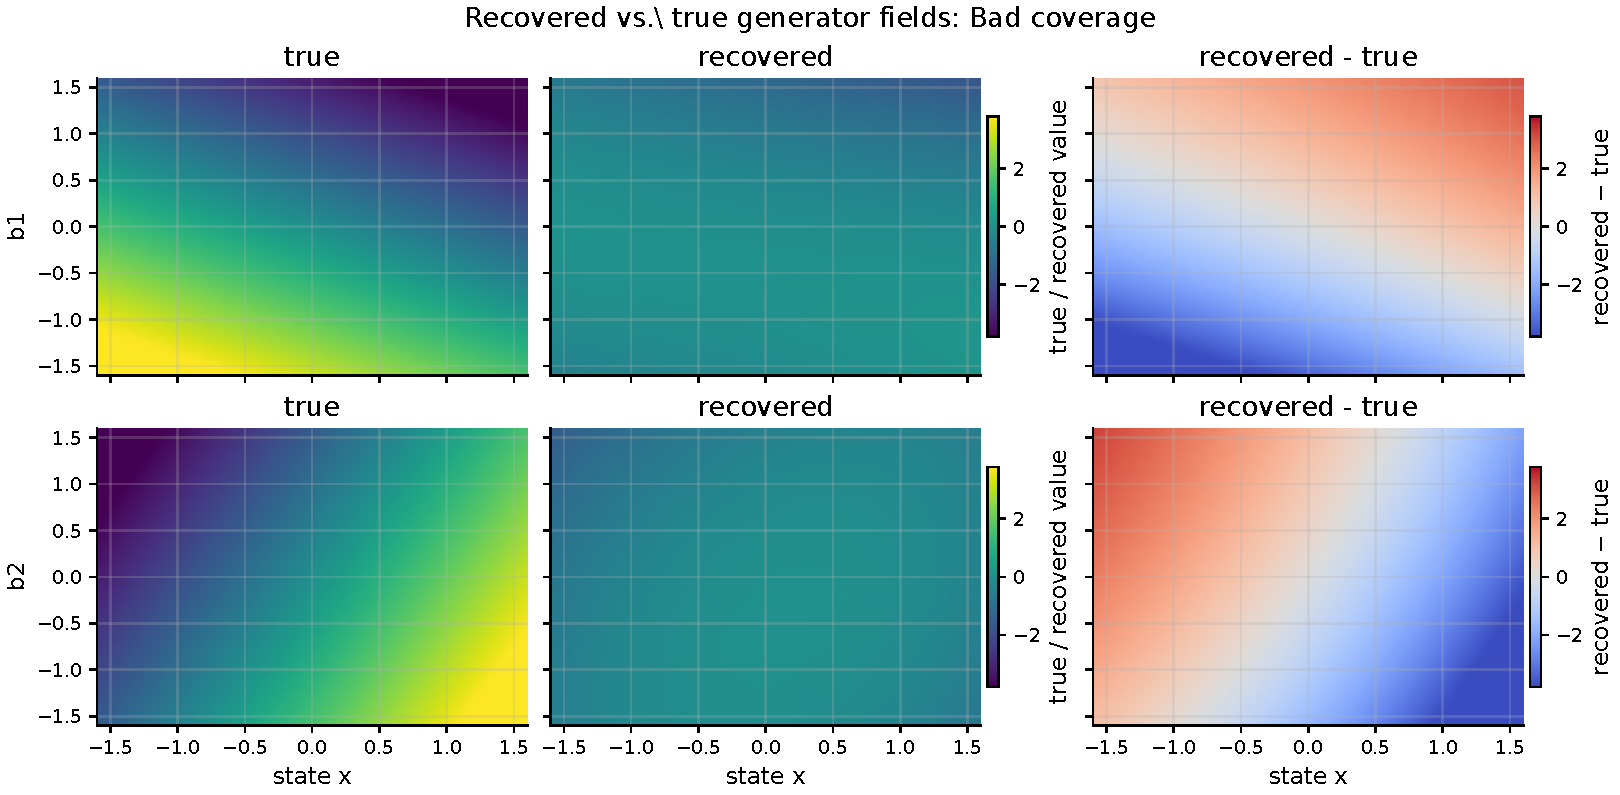
\includegraphics[width=0.86\linewidth]{datasheet_fields_bad_coverage.pdf}
\caption{Bad coverage: recovered vs.\ true generator fields (shared per-field colour scale; error column centred at zero).}\end{figure}
\paragraph{Verdict.} Drift $L^2(\mu)=0.815$, tensor rel-$L^2=0.784$, $a_{12}$ cosine $n/a$, PSD $1.00$, FP $0$ ($n$ seeds). \textbf{NAMED_NULL}.
\medskip

\subsection{Too-large time step}\label{sec:v62-too-large-dt}
\paragraph{Context.} The same multiplicative-diffusion system sampled at a coarse time step ($\Delta t=0.05$), included to expose the finite-step (Euler--Maruyama) discretisation bias. The drift-squared correction is exact only as $\Delta t\to0$; its residual grows with the drift Lipschitz constant relative to the step, so this case marks the temporal-resolution boundary of reliable recovery.
\paragraph{System.} $$\text{Diagonal multiplicative sampled at }\Delta t=0.05.$$
\paragraph{Generator.} Finite-step (Euler) bias dominates at coarse $\Delta t$; the correction residual grows with the drift Lipschitz constant. Named limit.
\paragraph{Recovery.} WG-SINDy recovers the drift at relative $L^2(\mu)=0.098$ and the diffusion tensor at $0.119$ relative error; this system is reported as a named limit. This is a named limit (registry declared failure or stress case): recovery fails for a physical or identifiability reason (library incompleteness, low signal-to-noise, degeneracy, or coverage), not an estimator defect.
\begin{figure}[H]\centering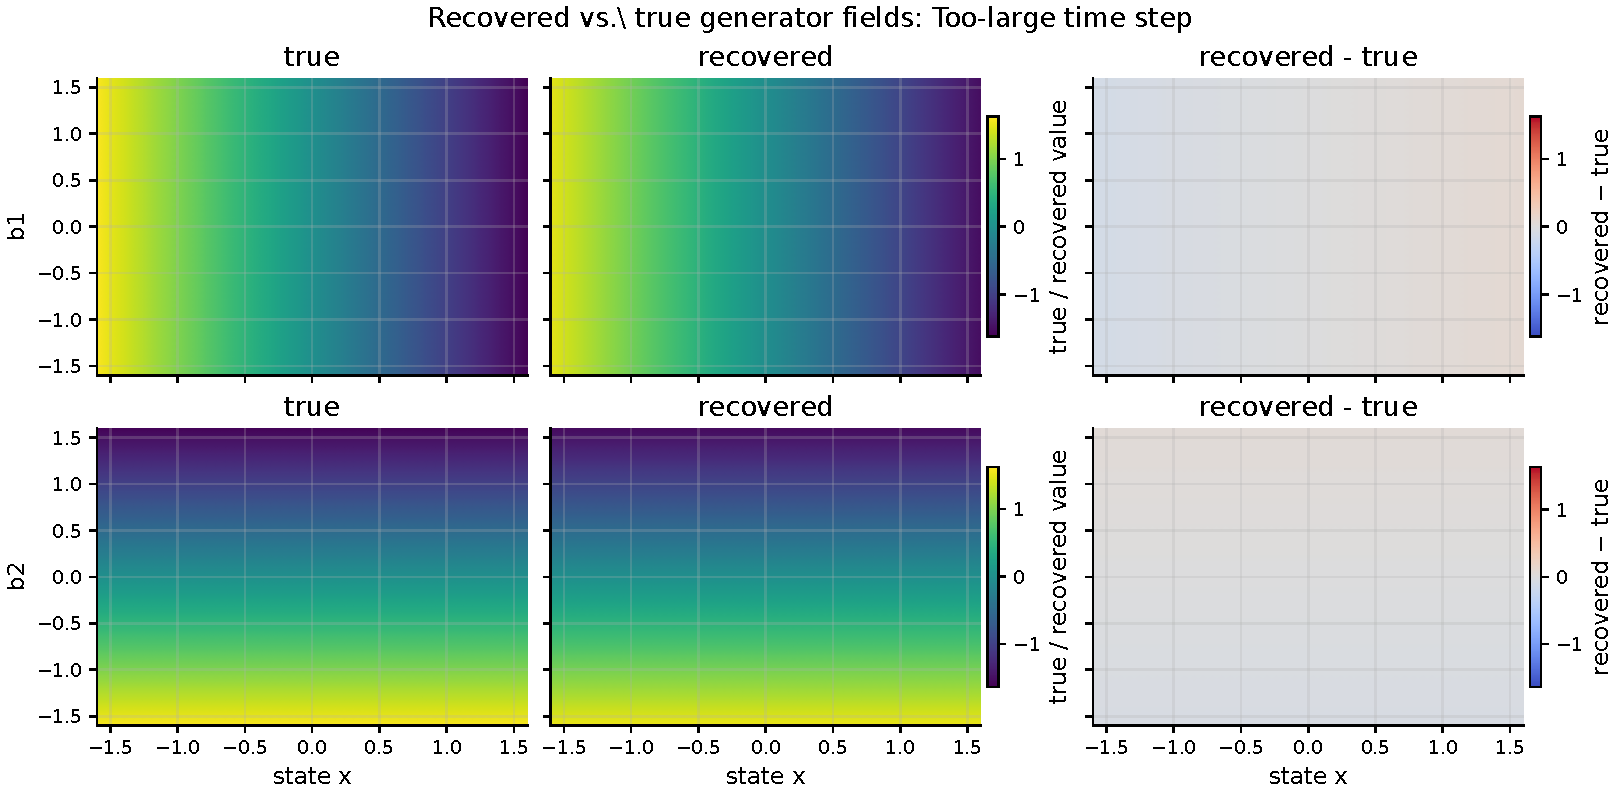
\includegraphics[width=0.86\linewidth]{datasheet_fields_too_large_dt.pdf}
\caption{Too-large time step: recovered vs.\ true generator fields (shared per-field colour scale; error column centred at zero).}\end{figure}
\paragraph{Verdict.} Drift $L^2(\mu)=0.098$, tensor rel-$L^2=0.119$, $a_{12}$ cosine $n/a$, PSD $1.00$, FP $0$ ($n$ seeds). \textbf{NAMED_NULL}.
\medskip
}{}


\end{document}
